%% ----------------------------------------------------------------
%% Thesis.tex -- MAIN FILE (the one that you compile with LaTeX)
%% ---------------------------------------------------------------- 

% Set up the document
\documentclass[a4paper, 11pt, oneside]{thesis}  % Use the "Thesis" style, based on the ECS Thesis style by Steve Gunn
\graphicspath{{Figures/}}  % Location of the graphics files (set up for graphics to be in PDF format)
\usepackage{caption}
\usepackage{array}
\usepackage{anyfontsize}
\usepackage{sectsty}

% Include any extra LaTeX packages required
\usepackage[square, numbers, comma, sort&compress]{natbib}  % Use the "Natbib" style for the references in the Bibliography
\usepackage{ragged2e}
\usepackage{float}
\usepackage{verbatim}  % Needed for the "comment" environment to make LaTeX comments
\setcounter{tocdepth}{5}
\usepackage[table, svgnames, dvipsnames]{xcolor}
\usepackage{longtable}
\usepackage{makecell, cellspace, caption}
\setlength\cellspacetoplimit{3pt}
% \usepackage{vector}  % Allows "\bvec{}" and "\buvec{}" for "blackboard" style bold vectors in maths
\usepackage{tikz}
\def\checkmark{\tikz\fill[scale=0.4](0,.35) -- (.25,0) -- (1,.7) -- (.25,.15) -- cycle;} 
\usepackage{array}
\newcolumntype{L}[1]{>{\raggedright\let\newline\\\arraybackslash\hspace{0pt}}m{#1}}
\newcolumntype{C}[1]{>{\centering\let\newline\\\arraybackslash\hspace{0pt}}m{#1}}
\newcolumntype{R}[1]{>{\raggedleft\let\newline\\\arraybackslash\hspace{0pt}}m{#1}}
\makeatletter
\newcommand\subsubsubsection{\@startsection{paragraph}{4}{\z@}{-2.5ex\@plus -1ex \@minus -.25ex}{1.25ex \@plus .25ex}{\normalfont\normalsize\bfseries}}
\newcommand\subsubsubsubsection{\@startsection{subparagraph}{5}{\z@}{-2.5ex\@plus -1ex \@minus -.25ex}{1.25ex \@plus .25ex}{\normalfont\normalsize\bfseries}}
\makeatother
\usepackage{url}
\usepackage{natbib}


\hypersetup{urlcolor=blue, colorlinks=true}  % Colours hyperlinks in blue, but this can be distracting if there are many links.

% remove the unnecessary spacing before and after the headings/subheadings
\usepackage[compact]{titlesec}
\titlespacing{\section}{0pt}{*0}{*0}
\titlespacing{\subsection}{0pt}{*0}{*0}
\titlespacing{\subsubsection}{0pt}{*0}{*0}

\setlength{\parskip}{6pt}
%\setlength{\parsep}{0pt}
%\setlength{\headsep}{0pt}
%\setlength{\topskip}{0pt}

%% ----------------------------------------------------------------
\begin{document}
\frontmatter	  % Begin Roman style (i, ii, iii, iv...) page numbering

% Set up the Title Page
\title  {Virtual Reality Based E-Commerce Web Application}
\session {2019-2022}
\advisor {Dr. Amna Zafar}
\coadvisor {Farwa Batool}
\authors {
Muhammad Ali Mazhar Butt ~~~ 2019-CS-224 \\
			 Abdullah Rasheed ~~~ 2019-CS-246 \\
			 Maham Wajid ~~~ 2019-CS-207\\
    Ehtesham Haider ~~~ 2019-CS-218 
    }

\addresses  {\deptname \\ \univname}  % Do not change this here, instead these must be set in the "Thesis.cls" file, please look through it instead
\date       {\today}
\subject    {}
\keywords   {}

\maketitle
%% ----------------------------------------------------------------

\setstretch{1.3}  % It is better to have smaller font and larger line spacing than the other way round

% Define the page headers using the FancyHdr package and set up for one-sided printing
\fancyhead{}  % Clears all page headers and footers
\rhead{\thepage}  % Sets the right side header to show the page number
\lhead{}  % Clears the left side page header

\pagestyle{fancy}  % Finally, use the "fancy" page style to implement the FancyHdr headers


%% Select only one of the certification pages  
%\CertificationMSc{}
\CertificationBSc{}
\clearpage  % Certification ended, now start a new page


%% ----------------------------------------------------------------
% Declaration Page required for the Thesis, your institution may give you a different text to place here
\Declaration{
%\addtocontents{toc}{\vspace{1em}}  % Add a gap in the Contents, for aesthetics
We declare that the work contained in this thesis is our own, except where explicitly
stated otherwise. In addition, this work has not been submitted to obtain another
degree or professional qualification.
\bigskip

Signed:~~ \rule[0em]{10em}{1.0pt} \\ % This prints a line for the signature 
Date:~~~~ \rule[0em]{10em}{1.0pt}  % This prints a line to write the date

}
\clearpage     % Declaration ended, now start a new page

%% ----------------------------------------------------------------

\setstretch{1.3}  % Reset the line-spacing to 1.3 for body text (if it has changed)

% The Acknowledgements page, for thanking everyone
\acknowledgements{
%\addtocontents{toc}{\vspace{1em}}  % Add a gap in the Contents, for aesthetics

First and foremost, we would like to praise Almighty Allah, the Most Gracious, and
the Most Merciful for His blessing given to us during our study and in completing
this project.
It gives us great pleasure to express our sincere gratitude and respect to our supervisor,
Dr.Amna Zafar, and co-supervisor Farwa Batool, for their patient
guidance, and enthusiastic encouragement, and for boosting our morale through all the
stages of this work. We could not have made it through without their constructive
suggestions, continuous support, and efforts. We would also like to appreciate the
Department of Computer Science, UET Lahore, and its staff for providing us with
an opportunity to work on and complete this project.
Finally, we would like to give special thanks to our parents for their genuine affection
and encouragement. It would not have been possible without their consistent
support and prayers for us.\ldots

}
\clearpage  % End of the Acknowledgements

%% ----------------------------------------------------------------
% End of the pre-able, contents and lists of things
% Begin the Dedication page
\setstretch{1.3}  % Return the line spacing back to 1.3
\pagestyle{empty}  % Page style needs to be empty for this page
\dedicatory{Dedicated to Allah Almighty for His blessings and
benevolence. We would also like to dedicate this project
and Final Year Project to our supportive families, and
friends who stood by us in times of need.\ldots}


%% ----------------------------------------------------------------
\pagestyle{fancy}  %The page style headers have been "empty" all this time, now use the "fancy" headers as defined before to bring them back

%% ----------------------------------------------------------------
\lhead{\emph{Contents}}  % Set the left side page header to "Contents"
\tableofcontents  % Write out the Table of Contents

%% ----------------------------------------------------------------
\lhead{\emph{List of Figures}}  % Set the left side page header to "List if Figures"
\listoffigures  % Write out the List of Figures

%% ----------------------------------------------------------------
\lhead{\emph{List of Tables}}  % Set the left side page header to "List of Tables"
\listoftables  % Write out the List of Tables

%% ----------------------------------------------------------------
\setstretch{1.5}  % Set the line spacing to 1.5, this makes the following tables easier to read
\clearpage  % Start a new page
\lhead{\emph{Abbreviations}}  % Set the left side page header to "Abbreviations"
\listofsymbols{ll}  % Include a list of Abbreviations (a table of two columns)
{
% \textbf{Acronym} & \textbf{W}hat (it) \textbf{S}tands \textbf{F}or \\
\textbf{VR} & \textbf{V}irtual \textbf{R}eality \\
\textbf{AR} & \textbf{A}ugmented \textbf{R}eality \\
\textbf{SDK} & \textbf{S}oftware \textbf{D}Development \textbf{K}it\\
\textbf{FR} & \textbf{F}unction \textbf{R}equirements\\
\textbf{NFR} & \textbf{N}on \textbf{F}unctional \textbf{R}equirements\\
}

%% ----------------------------------------------------------------
% The Abstract Page
\addtotoc{Abstract}  % Add the "Abstract" page entry to the Contents
\abstract{
%\addtocontents{toc}{\vspace{1em}}  % Add a gap in the Contents, for aesthetics

 The Virtual Reality-based E-commerce Web Application is an advanced website inspired
by the meta verse concept. The unique thing about this web application is that it provides
virtual reality mode to the customer so that the customers can experience the real-time feeling of the e-commerce store if they have VR headsets. Without a VR headset, they
can visit the website and can also do a 3d virtual tour of the store. On the basis of
user body measurement inputs, we are also providing the best suggestion for the size
that will fit the customer's body. Other than these major functionalities this application is
delivering advanced features to the customers like advanced searching, User-friendly navigation,
Advanced Searching, Product Filtering, Latest news section in which the latest
discount and sales will be displayed to the customer, Conversion of currencies to different
country’s currencies etc.\

}
\clearpage 
\thispagestyle{plain}
% Abstract ended, start a new page
\addtotoc{Executive Summary}
\begin{center}
{\huge \textbf{Executive Summary} \par}
\end{center}
Online shopping has become a major trend nowadays. Customers prefer it rather than going shopping physically as it is less costly and less time-consuming. That is why many shopping stores are going digital and enabling E-commerce features in their setup. However, customers face issues and satisfaction is less while shopping online as they cannot see how the product might look in reality. All they see is a 2d image, description, and reviews of previous customers. Showing 3d models of the products in the virtually created store which can be accessed through VR headsets can make the customers feel as if they are shopping physically. Metaverse concepts are used for this application. So Virtual reality-based E-Commerce store is created that would provide a positive and realistic experience to the customers in the metaverse. The core technology is virtual reality.
First, we create a basic E-commerce website named MetaMart with all related features and functionalities. Then 3d tour and VR mode that is created in Unity 3D is integrated with the website. For VR mode, an oculus headset is required. Initially in the application, garments, and outerwear will be the main products. 3D garments will be placed upon avatars with customized measurements so that customers can map them to themselves and choose the best suitable one. In this way, customers can explore MetaMart with virtual reality functionalities so that they can experience this innovative way of buying products satisfactorily by roaming around the store and viewing products that are mostly garments in 3D view and exploring the latest Metaverse technology in the application.
\clearpage  % Executive summary, start a new page
%% ----------------------------------------------------------------
\mainmatter	  % Begin normal, numeric (1,2,3...) page numbering
\pagestyle{fancy}  % Return the page headers back to the "fancy" style
\onehalfspacing
% Include the chapters of the thesis, as separate files
% Just uncomment the lines as you write the chapters

% Chapter 1

 % Write your own chapter title

\begingroup%
\makeatletter%
\let\clearpage\relax% Stop LaTeX from going to a new page; and
\vspace*{\fill}%
\vspace*{\dimexpr-50\p@-\baselineskip}% Remove the initial (default) 50pt gap (plus 1 line)
\chapterfont{\centering}
\chapter{Introduction}
\vspace*{\fill}%
\endgroup


\newpage
\label{Chapter1}
\lhead{Chapter 1. \emph{Introduction}} % Write in your own chapter title to set the page header

\section{Overview of the Project}
\justifying
We are making a Virtual Reality based E-commerce web application. This project is inspired by the meta-verse concept. The previous E-Commerce work never used any virtual stores or virtual environments in which different products were placed and customers can visit virtual stores in their homes just by wearing VR headsets. Currently, no website is having a virtual environment where customers can come with or without a VR headset and shop for wearable or other products just like they are shopping physically at the store. As for buying outerwear, customers have two options i.e to order online or to go to the mall or store. Another option is augmented reality in which the customer just opens up the camera and tries on different outfits \\ We will be catering to two types of customers, the ones having VR headsets will be able to visit the virtual store while wearing a VR headset where the customer can touch, and hold different products and can move in the virtual store. If the customer wants to try different outerwear like jackets so they can check the outerwear on their related Avatar in the virtual store and can experience it from all angles. Customers without VR headsets can visit the website and avail themselves of the virtual tour of the store where they don’t need any VR headsets. So basically, our modules consist of an E-commerce website, a Virtual tour environment, a Virtual Reality Environment that requires a VR headset, and proper and customized measurements of avatars and products so that customers can map them to themselves for a better virtual shopping experience.// Other than these, this application is providing advanced features to the customers like User-friendly navigation, Advanced Searching, Product Filtering, the Latest news section in which the latest discount and sales will be displayed to the customer, Conversion of currencies to different country’s currencies, etc.\\
\section{Background}
\justifying
In the previous already existing applications, implementation of the virtual reality mode of the E-commerce store was missing. It means the custosmers can see only the 2D images and lengthy descriptions of the product. Hence, there was a gap between the virtual and physical visits to the E-commerce store. Customers have to go to the store physically for a better experience of buying products. We overcome this situation by making an application in which we are going to implement 3D virtual reality mode and a 3D virtual tour of the E-commerce store integrated with the website having multiple features that every E-commerce website has. One huge feature that is going to be implemented is the customized product sizes for customers so that they can choose products according to their body measurements and requirements and experience this metaverse way of shopping to the next level.
\section{Problem Statement}
\justifying
There exists a huge gap between physical shopping and online shopping through web/mobile applications. To bridge the gap between the physical and digital worlds we are creating a virtual reality-based E-Commerce store that would provide a positive and realistic experience to the customers in the metaverse.
\section{Motivation}
\justifying
Our motivation is customer satisfaction by visiting the 3D virtual store in meta verse made with the latest technologies. Because there are lots of issues while visiting the shopping mall like time, conveyance issues, etc. So we are providing a positive digital virtual experience of shopping where customers with Oculus VR headsets can experience shopping that will be closer to real-time shopping in the shopping mall.\\
On the other hand, customers without VR headsets can do a virtual tour of the 3D E-commerce store. Based on customers’ body measurements, they can also map their sizes and choose a suitable product by customized measurements of avatars and other products.
\section{Objectives of the Project}
\justifying
Our objective is to remove the huge gap in the customer experience of online and physical shopping by introducing the virtual reality of the E-commerce store and providing real-time feeling to the customer with the help of a 3D virtual reality store and 3D Tour of virtual store. \\
The main objective is to create a VR-based E-commerce environment with the state of the art technologies to revolutionize the experience for online shopping experience for customers by introducing metaverse. One of our objectives is also to provide personalized customized fitting solutions for individual customers by introducing Meta-verse concepts and technologies.
\subsection{Industry Objective}
\justifying
Our industrial objective is to commercialize this application. This web application is to sell products in a virtual E-commerce store in Metaverse. But this application can be extended to other fields such as education, healthcare, etc. For example, some virtual online schools in our metaverse can be added. 
\subsection{Research Objectives}
\justifying
We are doing research on Meta verse concepts and how the real-world experience could be created in the digital world using advanced tools and technologies to provide customized/personalized fitting solutions according to the individual customers' body measurements. We are going to use our best knowledge and advanced technologies and frameworks  to make a virtual 3D store in meta verse as there exists no E-commerce system that provides a virtual reality-based online store with digital versions of the actual product, virtual avatars with different sizes, and customized positive experiences. Virtual reality with advanced technologies will shape the future of electronic retailing.\cite{MARTINEZNAVARRO2019475}
\subsection{Academic Objectives}
\justifying
The technologies and tools that we are using in our project will help us in our advanced learning and will fulfill our academic objectives as well.
\subsection{Business objectives}
\justifying
Following are some of the business objectives of the virtual reality-based e-commerce web application:
\begin{itemize}
    \item Profit maximisation
    \item Sales maximisation
    \item Revenue maximisation
    \item Surviving in the market
%    \item Satisficing principle
\end{itemize}
\section{Rules and assumptions}
Following are rules and cases of assumptions that are assumed to be true while experiencing virtual reality mode working:
\begin{itemize}
    \item The customer has an Oculus VR headset and the configurations/setting for Oculus VR Headset is also done by the customer before going into VR mode.
\end{itemize}
Following are rules and cases of assumptions that are assumed to be true while normally working:
\begin{itemize}
    \item The internet connection is stable.
\end{itemize}
\section{Scope of the Project}
\justifying
To bridge the gap between the physical and Digital worlds by creating a Virtual Reality-Based E-commerce Store that would provide positive and realistic experiences to customers in the metaverse. Currently, this application is limited to E-Commerce but this web application can be extended for virtual reality-based healthcare and educational systems.
\section{ Target Audience}
\justifying
Our Virtual reality-based e-commerce web application is dealing with average as well as professional customers. Professional customers who don't have much time to buy outerwear by going physically to shopping malls can just experience 3d virtual e-commerce stores for buying outerwear. On the other hand, average customers can do a 3D virtual tour of the e-commerce store. Those customers who don't know which size bests fits suits them can also avail of the best fitting size suggestion on our website.
\section{Challenges}
\subsection{VR Headset cost}
\justifying
The Oculus VR Headset price is about two lac that is not easily affordable by us and without this VR Headset, it's impossible to experience the virtual reality mode of the e-commerce store. So, buying VR Headset was one of the biggest challenges during the project working.
\subsection{Integration of Web-based and Unity Framework}
This was the second biggest challenge for us during the project. Because it was the first time for us when we were going to integrate the web with the unity and also the helping material for this was not available too much and the configurations of the VR Headset might affect the integration process.
\begin{figure}[H]
    \centering
    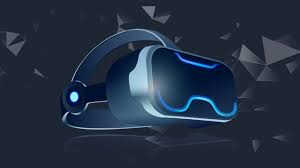
\includegraphics[width=15cm,height=10cm]{Figures/Others/VRHeadset.jpg}
    \caption{VR Headset}
    \label{VR HEeadset}
A head-mounted device used to experience virtual reality.  A hardware device that is connected to PC or mobile to experience VR environments and VR video games. VR headsets are mostly used in applications like trainers and simulators.
\end{figure}
\subsection{Configurations of VR Headset}
\justifying
To experience the virtual environment of unity in the oculus VR Headset we had to do configurations or settings in unity and it was not an easy task for us as after these configurations we were also going to integrate the unity environment with the Web.
\subsection{Understanding of payment API Integration}
\justifying
In our project, we used payment API for the first tie. It was quite difficult for us because this was the first time when we were going to integrate payment API in some web applications.
\subsection{Understanding how to integrate the processes}
\justifying
One of the challenges during project making was how to integrate the processes and what will be the sequence of the processes.
\subsection{Understanding of delivery method}
\justifying
One of the challenges was the understanding of the delivery method like when the customer order the product(i.e jacket) then the product should be delivered to the customer and on the successful delivery, we also need feedback from the customer. So handling all of this alone for us is difficult and we need a third party like Tcs etc for the delivery purpose the selection process for delivery and its API integration was also a big task for us.
\section{Constraints}
\justifying
The constraint of Virtual reality-based e-commerce web applications is that without VR headsets the customer cannot avail of the virtual reality mode. Because without an oculus VR headset the customer is unable to go into the 3D virtual store in meta verse but he can only do 3D of the store.
\section{Limitations}
This Virtual reality-based e-commerce web application is currently limited to clothes(only outerwear i.e jackets) only but it can be extended to further items that are part of future work.
etc.
Following are some of the limitations of our system as follow:
\begin{itemize}
    \item Our Virtual Reality based e-commerce store can work only on the desktop system, not on mobile phones or tablets, etc. 
    \item Real-time avatar creation through customer inputs is not currently implemented.
    \item Without a VR headset the virtual reality base e-commerce store cannot be experienced.
   % \item We had limited time to complete our project.
\end{itemize}

\section{Applications of Project}

\justifying
People can use this application to experience 3D virtual e-commerce at any place just by wearing an oculus VR headset. Without a VR headset customers can do a 3D tour of the store. Currently, our project is restricted to e-commerce only but it can be extended to various other fields as well like education, healthcare, buying and Decorating a House,
\section{Benefits of our Project to customer}

\justifying
Following are some of the possible applications of the virtual reality-based e-commerce web application:
\subsection{Better experience of buying a product online}
The customer without a VR headset like average customers can enjoy the 3D tour of the virtual 3D e-commerce store.
\subsection{Online 3D Tour facility}
The customer without a VR headset like average customers can enjoy the 3D tour of the virtual 3D e-commerce store.
\subsection{Ease to Customer}
This application will provide ease to the customer can experience the 3D virtual store by using an oculus VR headset at any location which can be home, office, etc. On the other hand, customers without an oculus VR Headset can also do a 3D virtual tour of the E-commerce store. The 3D images with 3D avatars will also give a realistic feeling to the customer and increase his/her engrossment.
\subsection{Customer Time Saving}
\justifying
It's a tedious task to go to a shopping mall and visit the whole store/mall to find your desired item. For example, you want to buy a jacket and you go to the mall and then visit the store to find your desired jacket. Let us suppose you did not find the desired one then you will have to return home and it's a real waste of time like you are wasting your time. Through this application, people can just experience a real-time 3D Virtual E-commerce store by using an oculus VR headset at any location which can be a home, office, etc. % Introduction 
\newpage

% Chapter 2
\begingroup%
\makeatletter%
\let\clearpage\relax% Stop LaTeX from going to a new page; and
\vspace*{\fill}%
\vspace*{\dimexpr-50\p@-\baselineskip}% Remove the initial (default) 50pt gap (plus 1 line)
\chapterfont{\centering}
\chapter{Literature Review}
\vspace*{\fill}%
\endgroup

\newpage
\label{Chapter2}
\lhead{Chapter 2. \emph{Literature Review}} % Write in your own chapter title to set the page header

\justifying
In this section, we are going to discuss virtual reality, applications that did work on E-Commerce applications with VR, AR, and a comparison of different web applications.
\section{Details of Existing Work}
\justifying
We are living in an era where technology is evolving at a rapid pace and so is the traditional way of work or business. For example, On-site classes are slowly switching to online classes, cash-on-hand payment is slowly switching to online payment, manual Registration, reservations, booking, etc are also being switched to online, so technology has greatly affected our traditional tasks. Now, it is evolving to virtual reality-based works to facilitate the users even more than before. The term “metaverse” has been on-trend in recent times. It is a concept in which people can collaborate and live their life virtually in the virtual world using VR headsets. So far it is in the initial stages but many single-purpose apps have already implemented this feature. In our relevant cases, many e-commerce and clothing stores have started working on this virtual try-before-you-buy feature. Usually, the try-before-you-buy technique is used by customers when shopping physically but many stores such as \cite{IkeaWala} Ikea have started Kitchen virtual reality in which a person can walk freely and interact with the virtual kitchen using a VR headset. Virtual 3-D Kitchen items can be tested in this environment. They also \cite{ekIkeaWala} has launched a new augmented reality application that allows users to test their products in real-time. So far it can only be used with Apple technology(ARKit). The app automatically scales products based on the given environment with 98 percent accuracy.
The E-Commerce websites like Amazon, Alibaba, AliExpress, Walmart, etc., and outerwear websites like Zeitgeist, breakout have traditional approaches where customers go on the websites and then see different product items and add to card method.
In today’s modern world, the need for technology with an E-commerce system has become a basic need. People need a more personalized and immersive shopping 
experience which makes the way for the meta verse concept. With the expansion of the industrial metaverse, Virtual shopping still needs learning, priorities,
 and insights for experience delivery \cite{"FutureofE-Commerce"}
\section{What is Virtual Reality?} 
\justifying
Virtual Reality is the future and it's a 3D complete environment in which everything provides a real-time feeling. Virtual reality is a buzzword today and it is popular nowadays in the future students can take lessons and classes in a virtual environment and companies like Amazon is also working on e-commerce virtual reality-based application. People can just wear a VR headset and in their homes, they can go to virtual e-commerce stores, and explore mental health treatment. There are lots of applications of virtual reality like VR in fashion design, mental health treatment, education, sports, military, medical training, etc.

\section{Difference between Virtual Reality and \\ Augmented Reality}

\justifying
No external AR headset is required for experiencing augmented reality while a VR headset is required for experiencing a virtual environment. In virtual reality, everything is virtual like objects in a virtual environment while Augmented reality augments the real-world scene. Snapchat uses augmented reality when we open a Snapchat camera then Snapchat provides different filters in which we can different objects The filters in which Snapchat lens scans our face and applies different cartoon shapes or filters or face changers etc. all possible because of augmented reality.

\section{Current State of Art}
        \begin{longtable}{| L{1cm} | L{2cm} | L{3cm} | L{2cm} | L{4cm} |}
            \hline
            \rowcolor{Gainsboro!60}
            \makecell{ } & \makecell{Name}  & \makecell{Category} & \makecell{Status} & \makecell{Function}
            \endhead
            1&	Yihaodian	& AR Store & Onsite&	AR stores created on open spaces that give customers the experience of real-world stores in smartphones .\cite{Yihaodian} \\
           \hline
2	& IKEA	& Catalog Application	& Online &	Customers can use AR technology in their smartphones to preview how furniture will look in that surrounding by augmenting furniture objects in real-world \cite{IKEA}\\
           \hline
3	& Lacoste	& LCST Augmented Reality Retail Campaign &	Online	&Customers can try different shoes . \cite{Lacoste}\\
           \hline
4	& Audi	& VR-Based Application &	On-Site	& Passengers traveling with a driver and feeling bored can experience amusing 3D environments configured with real-world vehicle speed, and bumps on the road in the real world by wearing VR headsets provided by AUDI .\cite{Audi} \\
           \hline
                5	& Converse	& Shoe Sampler & 	Online	& Customers can try shoes by using AR-based applications.\cite{Converse} \\
           \hline
6 &	Topshop	& AR Mirror &	In-Store &	Customers can try-on outfits in-store by using AR change room. \cite{Topshop}\\
           \hline
7 & Sephora &	AR-based application &	Online	& Customers can get virtual makeup and try different shades by using Sephora virtual assist in their mobile phones\cite{Sephora} \\
           \hline
8 &	L’Oréal	& AR-based application	& Online &	Customers can try out all L’Oréal products by using virtual makeovers and can try different beauty trends on their mobile phones, and tablets.\cite{Loreal}\\
           \hline
           9	& Burberry &	Virtual Store	& Online	& Customers will experience the virtual store by navigating through the 3D store environment and would be selecting products by selecting digital icons in the environment. \cite{Burberry} \\
           \hline
10	& Mister Spex	& Virtual Mirror &	Online	& Customers can try different frames of glasses virtually using AR-based applications and can find his/her favorite model.\cite{MisterSpex} \\
           \hline
         11 &	Timber Land	& AR Magic mirror	& In-Store &	Customers can tryout different outfits by standing in front of their avatar in mirror screen .\cite{TIMBERLAND}\\
           \hline
 12 &	Uniqlo &	AR Mirror 	& In-Store &	Customers can try different colors of a single cloth product by just wearing that single product in front of an AR-based mirror called “magical mirror”.\cite{UNIQLO}    \\
           \hline
13	& Gapinc &	AR-based application	& Online &	Customers can virtually try on clothes using an AR app called Dressing Room by GAP\cite{Gapinc} \\
           \hline
           \caption{
           Comparison of existing AR and VR-based applications.}
        \end{longtable}

This table discussed the existing AR/VR-based applications and their functionalities. These applications were developed by some famous companies like Audi, Converse, Sephora, and many others listed in the table. These companies brought new innovations to their respective field by using AR/VR technology. Such that Audi developed an application to kill the boring time of their users by providing them with a VR headset with amusing VR environments. The fusion of these amusing and enjoyable VR environments with car speed, acceleration and road bumps, and cuts made Audi’s customers attracted to this innovation.      
%\end{landscape}

\subsection{IKEA}
\justifying
IKEA made an application that used augmented reality by which customers can place the IKEA furniture at any place and can see how it will look at that place. For example, if you want to see how the table will look in your room then using the IKEA application you just have to open the camera same as Snapchat, and then you can see the place the object anywhere. So customers can place different IKEA furniture in any place like in their home. They just have to open the IKEA application and select a product and using the back camera of their mobile phone they can see how the furniture i.e table will look in their room. \cite{IKEA}
\subsection{Yihaodian}
Yihaodian is launching a virtual online grocery store based on augmented reality where customers. Yihaodian is one of the largest grocery online stores that work on buying groceries with AR experience to improve customer satisfaction and customer experience of buying products online.
\cite{Yihaodian}
\subsection{Lacoste}
\justifying
Customers can try different shoes with AR experience.
Using our extensive AR experience we developed a LCST app allowing consumers to “Bring the Colour” to their city by scanning store window displays, in-store signage, and promotional postcards to reveal exclusive 3D video animation content to consumers across 6 global territories. The AR activity helped successfully launch the new Lacoste streetwear brand by showcasing LCST as the bold, edgy choice in the urban sportswear market.\cite{Lacoste}
\subsection{Audi}
	Audi has developed a project named “holoride” in which they have tried to improve passenger rides. They have stated the problem situation when someone travels with a driver in an Audi car. At that time driver enjoys the ride but the passenger considers that time as wasted time. So Audi has tried to kill that boring time with a unique AR/VR experience. So they have used “Extended Reality(XR)” to build some beautiful and enjoyable VR experiences that passengers can experience while having a ride just by wearing a VR headset. 
The cool thing in this “holoride” is the relationship between the real world and the virtual environment. In the virtual world, passengers will be riding on some 3d objects like a cart, or an animal-like dinosaur based on the VR environment the passenger would be in. So there would be a fusion of real-world data with a VR environment such that the speed of the ride in the environment would be the same as the speed of the car in the real world. Similarly, with each bend on the road, with each application of the brake, the virtual reality experience would be shaped just like the real world. 
They have just replaced the boring passenger experience of the real world with a fascinating, colorful, and amusing virtual reality experience. \cite{Audi}

\subsection{Converse}
 The converse is a shoemaker company that has created an AR app to ease users with a fitting facility without leaving home.
Converse not only solved customers’ pain but also reduced its sales funnel. They have created an AR app in which users can see if the shoes fit him/her by using AR technology. The user just has to open the AR camera and select his/her favorite shoes and just point the camera toward his feet to see shoes fit or not.
There was a gap in online shoe shopping which was size fitting. But this technology eliminated this gap in online shopping.
 \cite{Converse}
 
\subsection{Topshop}
TOPSHOP a renowned fashion brand launched an augmented reality shopping tool, TOPSHOP Kinect, that helps their customers to try on their selected collections in an augmented dressing room. They worked with the Russian agency AR Door and launched the augmented reality dressing room in Moscow. They use Microsoft's Xbox Kinect software to create virtual mirrors.
Users simply must pose with their arms headed upward and allow the Kinect to take the picture. Then viewers can move their hands and check different styles that are inside the application. Kinect’s built-in camera scans the body and places the selected dress concerning the user's every movement. Its changing room is the first of its kind to hit major retail stores.\cite{Topshop}
\subsection{Sephora}
\justifying
Sephora introduced a mirror-like application in which a person can test the makeup toolkit accurately with the actual motive to make the person through AR and not with the conventional technique. It checks for the precise location of a user’s facial features, making it to be the world’s first photo-realistic 3D mirror. Try-on technology and Digital dress-up are its two major functionalities. \cite{Sephora}
\subsection{L'Oreal}L'Oréal's Modiface brings an AI-powered Virtual Makeup setup. Customers can apply makeup and try different shades to use virtual artists on their mobile phones. ModiFace, a leader in augmented reality and artificial intelligence in the beauty industry provided its AI-powered technology for cosmetic try-on virtually.
\cite{Sephora}
\subsection{Burberry}
Burberry, a fashion house, collaborated with ELLE Digital Japan in its latest move to create an interactive virtual copy of the Ginza store. They upgraded themselves through creative innovations and explored the relationship between physical and digital experiences for creating new concepts.
Customers can now roam around the virtual store and purchase items from Burberry’s inventory.
The store is built over three floors: the ground floor contains signature bags. The first floor contains womenswear from key outerwear. The top floor includes menswear and outerwear. Burberry and ELLE Digital Japan and in collaboration with actress Elaiza Ikeda created styling films that can be accessed through the virtual store.\cite{Burberry}
\subsection{Mister Spex}
It provides an amazing experience in that you can see how different glass frames will look on you in the virtual mirror and this is all you can do in your home on the Mister Spex website.
\subsection{Timber Land}
This clothing brand took the relationship with the audience and the experience to a new level. The mobile app was used initially for fitting in AR mode. Now people don't even have to go to the store. They just have to reach an 80-inch monitor and a full-length character appears on the screen. This approach resulted in a positive and incredible review by people and they started to use this AR fitting service in queues. Sharing of results of virtual fitting via Facebook and email is also possible.\cite{TIMBERLAND}
\subsection{Uniqio}
UNIQLO started initiatives to decrease environmental waste and support hawker culture, where people from over Singapore gather at hawker centers to dine. They created exhibition displays and augmented reality murals at UNIQLO stores. 
They provided an interactive experience by pointing to their mobile phones. Customers can also unlock face filters on Instagram after scanning the AR mural, granting them access to take selfies.
\\
The company aims to incorporate its efforts into eradicating environmental waste combined with AR technology. The company is looking to further its efforts into environmental waste, combined with newly released AR technology.\cite{UNIQLO}
\subsection{Gapinc}
Gapinc.Gap introduced Virtual Dressing and unveiled a new pilot app called the Dressing Room by Gap. The app was created to help customers virtually “try on" clothing through a smartphone, Augmented Reality experience. This is how it works – shoppers choose a Gap style that they might be interested in purchasing. Next, they select one of five body types featured in the app so they can “try on" the piece of clothing from anywhere on a Google Tango-enabled device, and if they love it, they can buy it online.
The fashion industry has not traditionally been geared toward helping people understand how clothes will fit. But Gapinc is determined and passionate about winning customer trust by consistently presenting and delivering products that make them look and feel great.\cite{Gapinic}

\section{Research Gap}
The previous E-Commerce work never used any virtual stores or virtual environments in which different products were placed and customers can visit the virtual store in their homes just by wearing VR headsets. In short, there is no current such a website that is having a virtual environment where customers can just come into the virtual store while wearing a VR headset and when a customer clicks on the dress he/she can see the avatars wearing the outfits like a jacket and the customer can also see the detailed information like different sizes of outfits (For example jackets). As to buying outerwear customers have two options first one is to order online and the second one is to go to the mall or store to buy outerwear. Another option is the augmented reality the customer just opens the camera and can try on different outfits because of the augmented reality. 
Another, gap we found is that there are 2D images of outfits and the models wearing those outfits are also in 2D images instead of the 3D model. Like a 3D image in which a person wearing outfits and customers can see back and forth how actually outfit will look like when any person will wear it.
            \begin{center}
             \captionof{table}{Research work on AR/VR}
\begin{tabular}{ | m{1em} | m{5em} | m{10cm} | } 
 \hline
 \textbf{} & \textbf{Research Paper Name} &
 \textbf{Description}  \\  \hline
           1 & The rise of 3D E-Commerce: online shopping gets real with virtual reality and augmented reality during COVID-19 & This paper has focused on some points which are listed below.
\begin{itemize}
    \item COVID-19 has affected the business field. All physical businesses are trying to shift towards online business.

\item 	E-commerce websites provide a well professional 2D website for online shopping but this is not enough for users.
 \item 	User must get the experience of the physical world (real world). So that they can make a good choice and can get a better experience.
 \item 	AR and VR technology increase customer satisfaction.
 \item 	Users can get more precise information using AR and VR technologies.
 \item 	User experience is increased by an AR assistant providing the user with all the required information in audio form or using an avatar.\cite{3DECommerce}
\end{itemize}

         \\  \hline

          2 & Multi-Dimensional Interface Design of E-Commerce for Virtual Museum System &
         \begin{itemize}
    \item 
          This research paper focused on the interface design of virtual museum systems.  \item The Paper suggested that interface design can be displayed in multi-dimensions.  \item The 2D view was good but not good enough as all the images of antiques are displayed in 2D in front of the user.  \item Navigation was difficult for human cognition. To make the system productive, panorama functionality was used. VR technology was used that makes users able to walk through the museum. Also, they provided the functionality of zooming to users.
 \item The result of this implementation was that information presented using VR and panorama technology was more effective as compared to 2D images. This increased usability of the system.
 \end{itemize}
 \cite{Multi-dimensionaldesign}
         \\  \hline
              \end{tabular}
\end{center}
\newpage
\begin{table}[H]
    \centering
\begin{tabular}{ | m{1em} | m{5em} | m{10cm} | } 
 \hline
 \textbf{} & \textbf{Research Paper Name} &
 \textbf{Description}  \\  \hline
           3& A Free Virtual Reality Experience to Prepare Pediatric Patients for Magnetic Resonance Imaging: Cross-Sectional Questionnaire Study & 
           \begin{itemize}
            \item A magnetic resonance image (MRI) is a test that requires patients to lie still until the test is done. 
 \item 	MRI is difficult for children to tolerate. So doctors use general anesthetic (GA) to ensure patient safety. 
 \item 	So this paper was written to make a VR resource that can be used to prepare patients for MRI by reducing their anxieties about the MRI process.
 \item 	This resource was consist of an app with a preparation book. This app used 360-degree videos of MRI machines to create a real-world simulation so that patients could be prepared for the real MRI test.
 \item In the end, the VR resource was smart enough for educating patients about the MRI process.\cite{VRExperienceInMedicalField}
\end{itemize}
       \\  \hline
          4 & Virtual Reality as an Educational and Training Tool for Medicine & Points which are discussed in this research paper are listed below
          \begin{itemize}
 \item 	There are two general classifications of Virtual reality. The first one is that in which we visualized the real world using 3D technologies like Unity. The second one is that which is a reflection of reality, the type of VR classification created using spherical or 360 images or videos. 
 \item 	This research paper explains both systems.
 \item 	Technologies used for these systems are Cardboard SDK and Gear VR SDK. 
 \item 	Cardboard SDK is used to create systems for a wide range of glasses and devices.
 \item 	Gear VR SDK is used to create a virtual experience for Gear VR 
 \item 	For the 360 content system Samsung gear 360 camera was used. 
 \item 	For visualized VR system Unity 3D gaming engine was used.
The system facilitated medical students to perform practices in the virtual world instead of with real patients.\cite{VirtualRealityInEducationandTraining}
\end{itemize}


         \\  \hline
     \end{tabular}
    \caption{Research work on AR/VR}
    \label{Table2.2: Research work on AR/VR}
\end{table}
This table discussed some research work on AR and VR technologies as well as the need to integrate these technologies with other fields like business and medicine. In the first paper effect of COVID-19 on business and how AR/VR can overcome the gap due to this pandemic is discussed. Similarly, the role of AR/VR technologies in the medical field is talked through in other papers. For example, VR technology was used to simulate the MRI process for children patients. So that they could lie still during the real-world MRI process.
\section{Functional Requirement}
      \begin{table}[H]
          \centering
         \begin{tabular}{ | m{8em} | m{10cm} | } 
 \hline
 \textbf{Functional Requirement Number} & \textbf{Description}  \\  \hline
           FR1 & 3D Virtual Store that can be experienced using VR Headset
         \\  \hline
           FR2 & 3D Virtual tour of E-Commerce Store
\\           \hline
           FR3 & 3D images/models instead of 2D images
        \\   \hline
           FR4 & Avatar in different measurements (height, weight, waist, etc.)  will be placed in a virtual store that will try the products (i.e jackets) that will be selected by the customer.
     \\      \hline
           FR5 & Website content translation to different Languages
     \\      \hline FR6 & Proper and concise details of products should be shown to the user in the virtual store as well on the website.
    \\       \hline FR7 & Conversion of currencies to different country’s currencies
    \\       \hline FR8 & 3Multiple Payment Options
       \\    \hline FR9 & User-friendly navigation
         \\  \hline FR10 & Advanced Security features like passwords, and credit card information will be stored in encrypted form in the database
         \\  \hline FR11 & Add to Wish List button
          \\ \hline FR12 & Rating and Feedback from the customer
          \\  \hline FR13 & Social Media Integration
          \\  \hline FR14 & When
          \\  \hline FR15 & Advanced Searching, Product Filtering
          \\  \hline FR16 & Special Offers and Discounts
          \\  \hline FR17 & Website content translation to different Languages
         \\  \hline FR18 & 3D images/models instead of 2D images
          \\  \hline FR19 & Latest news section in which the latest discount and sales will be displayed to the customer
         
     \\  \hline
     \end{tabular}
     
          \caption{Application’s functional requirements}
          \label{Application’s functional requirements}
          
      \end{table}
      
    This table discussed all the desired operations of the application. For example making 3D avatars, making 3D environments, and all other specifications on which the application is mainly concentrated are listed in the table.
\section{Non Functional Requirement}
Following are some of the non-functional requirements of our web application.
            \begin{table}[H]
                \centering
               \begin{tabular}{ | m{5em} | m{6em} | m{9cm} | } 
 \hline
 \textbf{NFR No.} & \textbf{NFR Name} &
 \textbf{Description}  \\  \hline
           NFR1 & Security & Passwords of customers must be in encrypted form.
         \\  \hline

           NFR2 & Scalability & The store shall support 10k to 15k users on a single server without harming the website speed and load.
         \\  \hline
           NFR3 & Maintainability & Because we are looking to grow, the website shall remove all the back-end complexities for in-house engineers to make changes to the system in the future.
       \\  \hline
           NFR4 & Usability & A customer should easily find the right product for them, understand what problems it solves, and purchase without contacting us.
         \\  \hline
     \end{tabular}

                \caption{Application’s non-functional requirements}
                \label{Application’s non-functional requirements}
            \end{table}
            This table discussed all the nonfunctional requirements of the application. For example scalability, maintainability, and usability as listed in the table. These requirements would be fulfilling some constraints e.g system must be able to support 10k to 15k users on one server without any negative impact on the system’s speed.
\section{Gap Analysis or Research Gap}
There is currently no website that is providing the Virtual reality mode customers are unable to visit and buy products at any sort of virtual 3D store in the metaverse just by wearing an Oculus VR headset. We are going to remove the gap in the customer experience of buying outerwear between physical means and online means by introducing a 3D virtual E-commerce store and a 3D virtual tour of the E-commerce store. Other than these major functionalities this application is providing advanced features to the customers like advanced searching, User-friendly navigation, Advanced Searching, Product Filtering, the Latest news section in which the latest discount and sales will be displayed to the customer, Conversion of currencies to different country’s currencies, etc.
\begin{figure}[H]
    \centering
    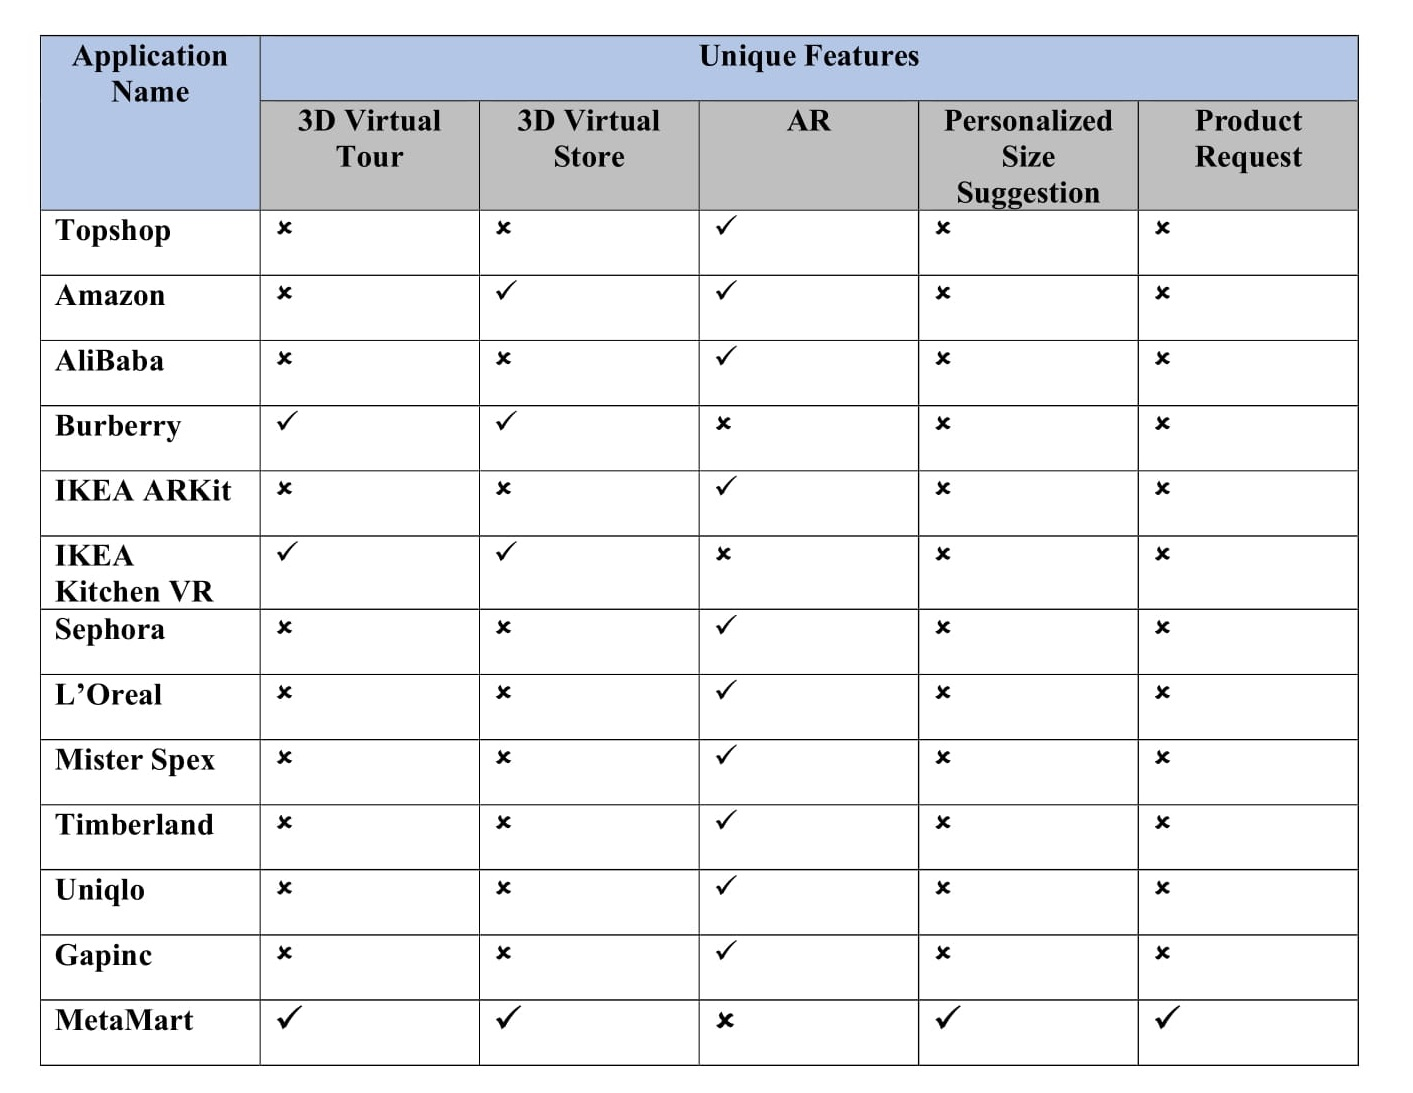
\includegraphics[width=15cm,height=15cm]{Figures/Others/ComparisonTable.jpg}
    \caption{Comparison of existing AR/VR application’s key features}
    \label{fig2:Comparison of existing AR/VR application’s key features}
    \justifying
   This table list some key features and their availability status in existing AR/VR applications. The table shows some features like a 3D virtual tour, 3D virtual store, AR, and personalized size suggestions. Every existing AR/VR application listed in the table has used some of these features not all. But our system would be focusing on all these features.
\end{figure}
 % What to Write 
\newpage

% Chapter 3
 % Write in your own chapter title
\begingroup%
\makeatletter%
\let\clearpage\relax% Stop LaTeX from going to a new page; and
\vspace*{\fill}%
\vspace*{\dimexpr-50\p@-\baselineskip}% Remove the initial (default) 50pt gap (plus 1 line)
\chapterfont{\centering}
\chapter{Proposed Methodology}
\vspace*{\fill}%
\endgroup

\newpage
\label{Chapter3}
\lhead{Chapter 3. \emph{Proposed Methodology}} % Write in your own chapter title to set the page header

\section{General Flow}
The web application we developed offers a wide range of key functionalities and is
easy to use. Our application is designed primarily for administrators and online
users having VR headsets and those who don't have VR headsets as well. The admin can add new products, delete products, update deleted products, view reports/statistics, customer lists, and pending and completed orders. The admin can also update his account setting if necessary. While on the other hand, the customer can visit the website with and without a VR headset as well. Those customers having Oculus VR headsets can experience virtual reality-based MetaMart while customers without VR headsets can do a 3D tour of the MetaMart. The customer can also request some products if not available in our store. Following are some of the diagrams that will help you to understand the sequence flow of our application.
\section{Software development methodology}
We are using Agile methodology.
\subsection{Road map}
Our main goal is to revolutionize the idea of E-Commerce business to facilitate the customer with an immersive and modern virtual platform to bridge the gap between the real and virtual shopping experience. So, to accomplish this goal we came after with the following steps:
\begin{enumerate}
    \item 	Exploring related existing past work (if any), wade through the research papers, articles, and generals. Endeavor to perceive the gaps of prior related works.
    \item Defining a working methodology, which software development approach we are going to manipulate throughout the whole development process.
    \item Specifying the functional and non-functional requirements for the targeted vision.
    \item Conducting feasibility study to contemplate all the aspects of the purposed application model to assemble an estimation is respect to accomplishment extent.
    \item Creating a general flow diagram to accentuate the workflow of the proposed application. Then, design several diagrams including a general diagram, data flow diagram (level0 and level1), use case diagram (general and detailed), flow chart, class diagram, entity-relationship diagram, and sequence diagram to clarify every aspect in a detailed way. 
     \item Note down all the use cases for the MetaMart application.
    \item Afterwards, select the tools and technology going to operate throughout the entire proposal implementation.
    \item Designing the wireframes for web configuration of the virtual environment.
    \item Designing a virtual 3D virtual store in meta verse , 3D clothes, 3D avatars.
    \item Designing the prototype to delineate an explicit scheme of how the proposed application is going to operate.
    \item Finally, developing the MetaMart website and integrating it with the 3D virtual environment made with Unity framework to make the complete system in a fine useable form.
    \item Testing the entire developed system and performing the test case scenarios and evaluating the project according to the test case scenarios.
\end{enumerate}
Feasibility Study:
i)	Economic feasibility:
1.  Web development: almost cost none.
2.  API: some APIs require purchase, so it will account for cost.
3.  Hardware: Our project requires some hardware devices (VR Headsets) which add to the cost of our project. So, to fulfill our economical requirements, we have applied for funding assistance on Ignite FYP funding assistance through the NGIRI portal.

\subsection{Technical feasibility}
The 3D virtual tour and 3D virtual store experience with a VR headset are achievable. With the help of currently available tools to us, it's difficult to make avatars with customized customer input sizes. Regular MetaMart with advanced features like advanced searching filtering, easy navigation, and social media sharing button integration can be done.

\subsection{Operational feasibility}
we will analyze whether our project will work accordingly in the same way as decided. we will also check whether all the features are implemented in the project. So, all the requirements will be fulfilled. we will also keep in the view that our website will be easy to use for customers and should be understandable.

\subsection{	Schedule feasibility}
As for the development process, we will follow the agile methodology in which we will design weekly sprints and in each scheduled meeting, we will improve our system timely. So in his way, the proper schedule will be followed and our product will be completed by the end within the due timeline.

\section{General Proposed Model}
\begin{figure}[H]
    \centering
    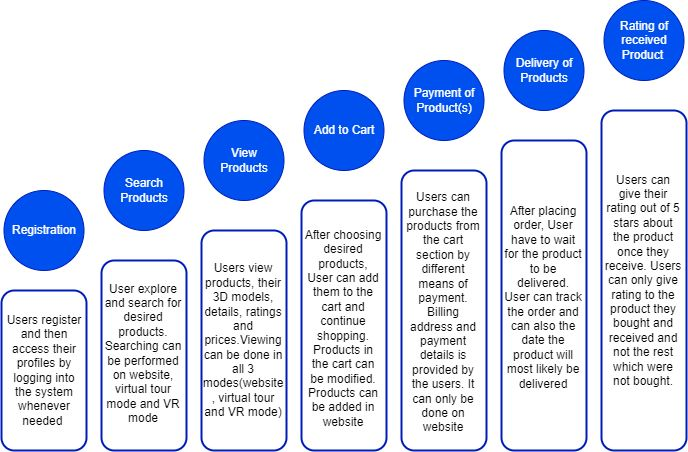
\includegraphics[width=15cm,height=10cm]{Figures/Diagrams/GeneralProposedModel.jpeg}
    \caption{General Proposed Model
     of Virtual Reality-based MetaMart Web Application
     }
    \label{fig: General Proposed Model}
   General Proposed Model
     of Virtual Reality-based MetaMart Web Applications.
\end{figure}
\section{Data Flow Diagram}
Following are the data flow diagrams of the Virtual reality-based MetaMart web application:
\subsection{Data Flow Diagram Level0}
\begin{figure}[H]
    \centering
    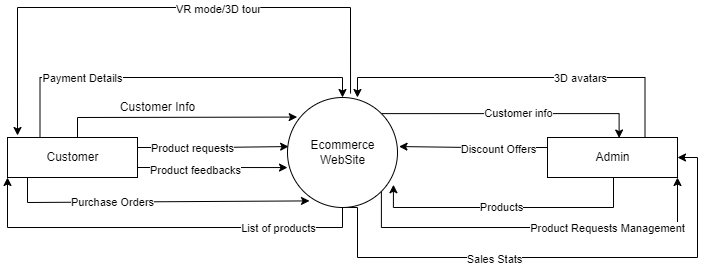
\includegraphics[width=15cm,height=8cm]{Diagrams/dfdlevel0.png}
    \caption{System’s Data Flow Diagram (Level-0)}
    \label{fig: System’s Data Flow Diagram (Level-0)}
\end{figure}
 \justifying
    This diagram illustrates the flow of data between 3 major components of the system which are the customer, admin, and web application. This figure describes which data would be flowing from which source to which destination. As some data like customer information would be flowing from customers towards the application. Similarly, product data would be entered by the admin so this data would be flowing from the admin toward the application. 
\subsection{Data Flow Diagram Level1}
\begin{figure}[H]
    \centering
    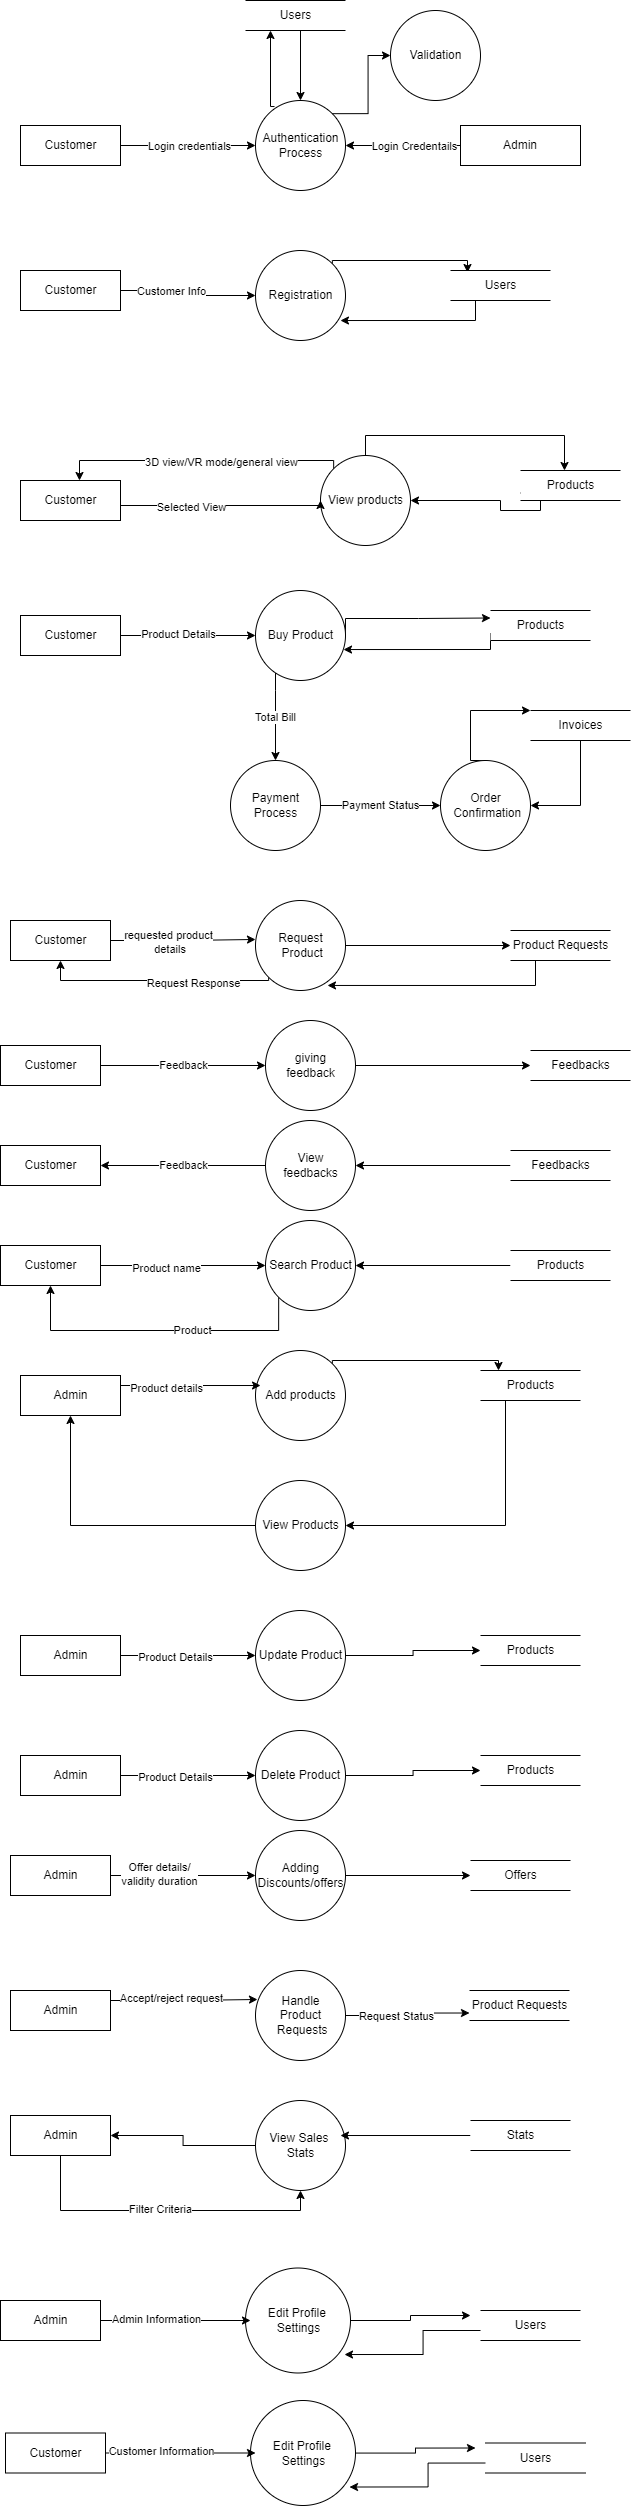
\includegraphics[width=12cm,height=25cm]{Diagrams/dfdlevel1.png}
    \caption{System’s Data Flow Diagram (Level-1)}
    \label{fig: System’s Data Flow Diagram (Level-1)}
\end{figure}
 \justifying
    This diagram illustrates the flow of data between the system’s components by reducing the abstraction level. In this diagram application component in the level-0 diagram is divided into some important modules like giving feedback, making an order, making payment, updating customers’ information, handling request, and many others shown in the diagram. All these modules represent the direction of data, the data which a module consumes or sends to any other dependent module or database.
\section{Use Case Diagram}
In the below section, you will see the General use case diagram and detailed use case diagram of the website as well that describe the high-level functions and scope of a system. 
\subsection{General Diagram}
\begin{figure}[H]
    \centering
    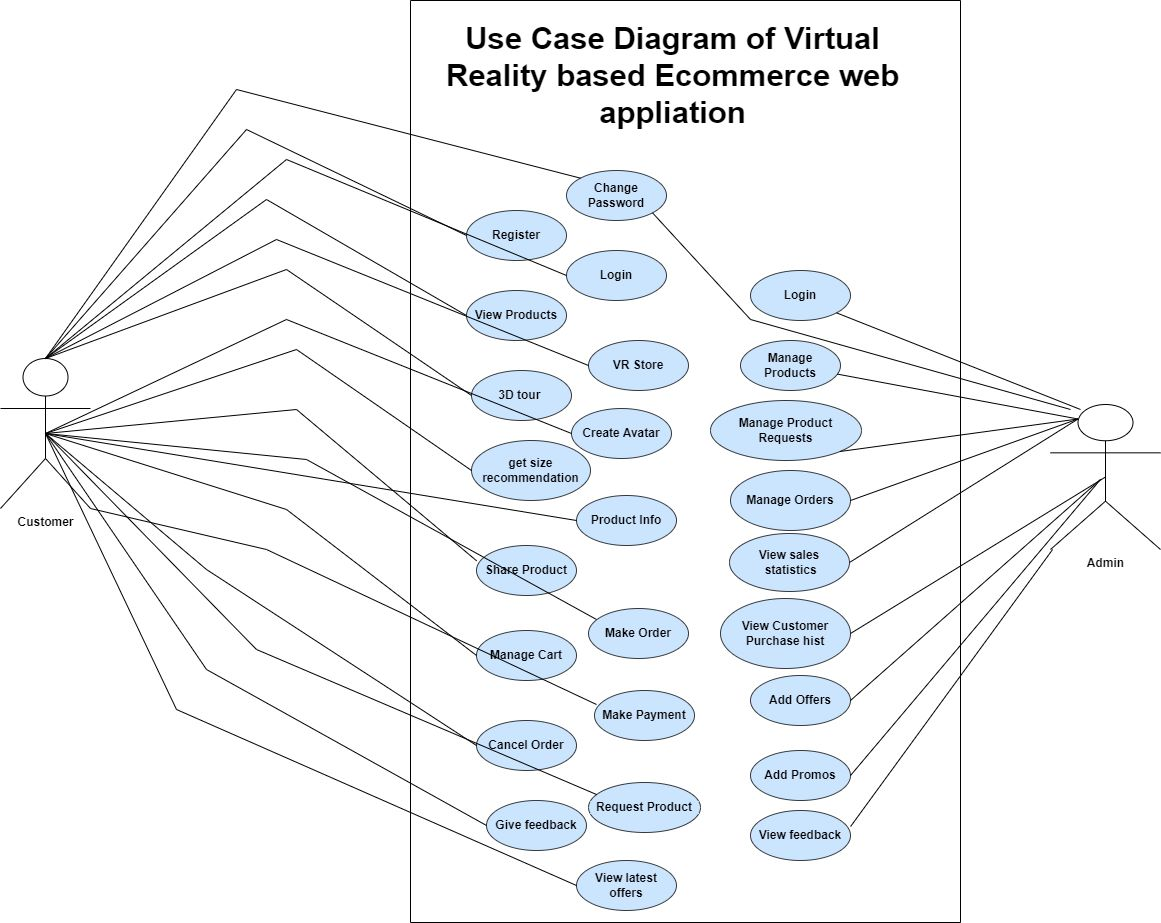
\includegraphics[width=15cm,height=15cm]{Diagrams/GeneralUseCaseDiagram.jpeg}
    \caption{General class Diagram}
    \label{fig: General Use case diagram}
   \justifying
   This diagram represents the general use cases with higher abstraction levels. All the use cases of entities(customer and admin represented by avatars in the diagram) are listed by associating them with the respective entity’s avatar. For example, login is a use case so this use case is associated with the admin’s as well as the customer’s avatar.
\end{figure}
\subsection{Detailed Use case diagram}
\begin{figure}[H]
    \centering
    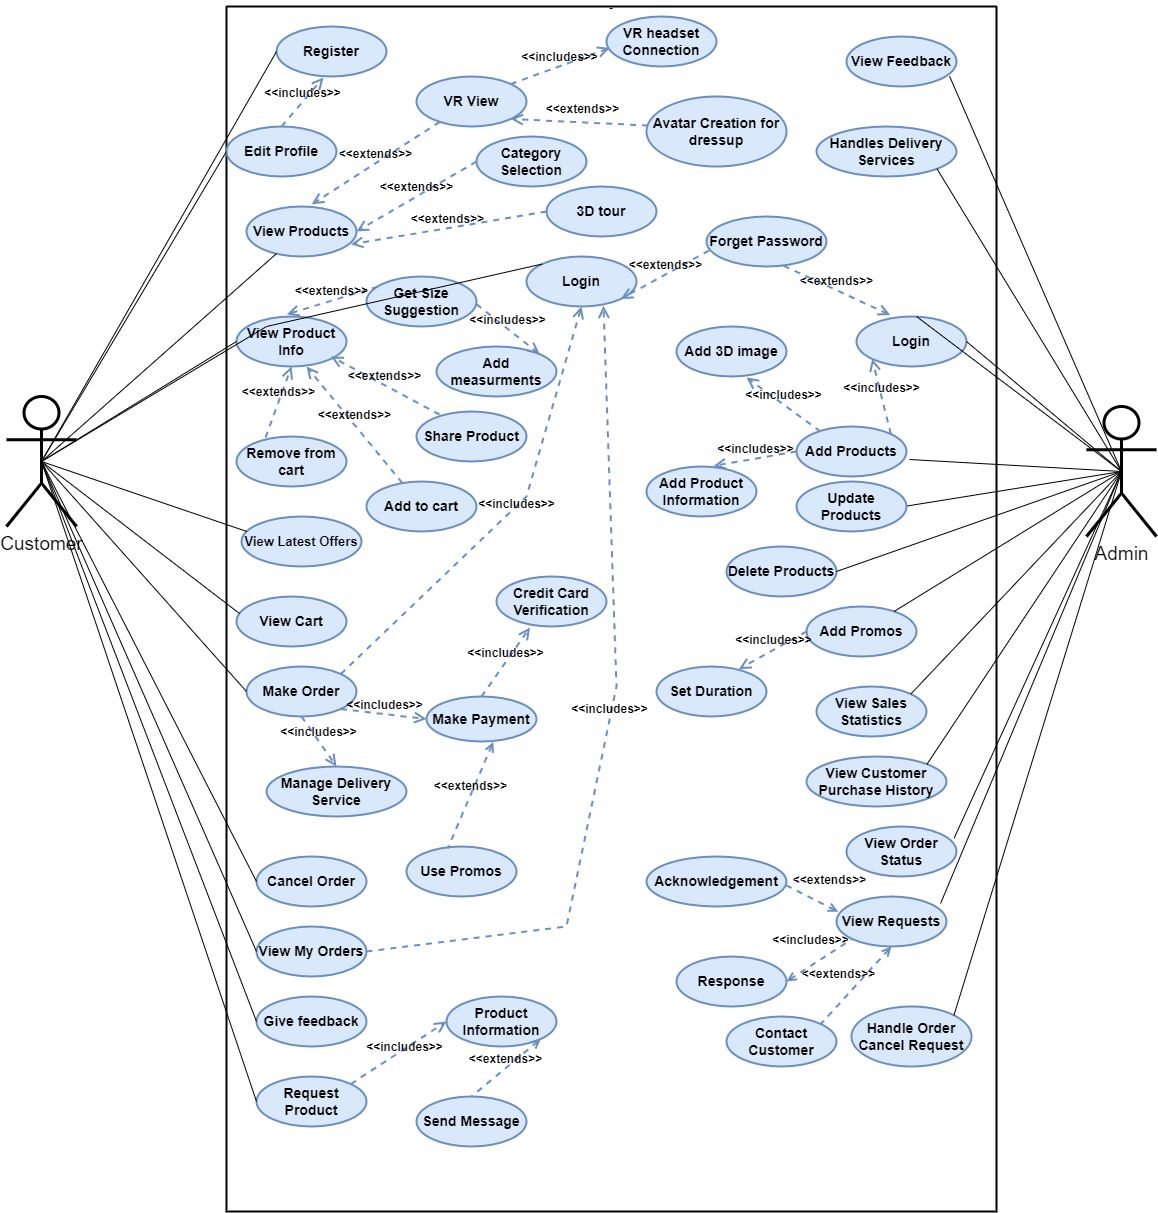
\includegraphics[width=15cm,height=15cm]{Diagrams/DetailUsedCaseDiagram.jpeg}
    \caption{Detailed Use case diagram}
    \label{fig: Detailed Use case diagram}
\end{figure}
\justifying
This diagram represents the detailed use cases. All the use cases of entities are listed along with the relationship(extend/includes) between use cases. For example, login is a use case but another use case which is forgetting the password extends this use case. Similarly, making an order includes making a payment because to complete the first use case (make order),  it is necessary to fulfill included use case which makes payment.
\section{Use Cases}
Following are the actors in our virtual Reality-based MetaMart web application:
\begin{enumerate}
    \item Admin
    \item Customer
\end{enumerate}
\subsection{Use Case of Admin Section}
\subsubsection{Use Case UC-1: Admin Login }
\textbf{Description:}\\
The following use case is about successful administrator login after providing valid login details.
\\
\textbf{Pre-Conditions:}
\begin{enumerate}
    \item Admin should have already been registered.
    \item  All required information about the admin should be available in the database.
    \item Databases should be available.
\end{enumerate}
\textbf{Normal Flow:}\\
\begin{enumerate}
\item The administrator enters valid login details.
\item Administrator clicks on the login button.
\item System confirms and validates the data. 
\item Admin successfully logins the account.
\end{enumerate}
\textbf{Post-Conditions: }
\begin{enumerate}
\item	Admin successfully logins the account. 
\end{enumerate}
\textbf{Authority:}
Administrator
\subsubsection{Use Case UC-2: Add Products }
\textbf{Description:}\\
The following use case is about managing and adding products to the existing system.
\\
\textbf{Pre-Conditions:}
\begin{enumerate}
    \item  All required information about the admin should be available.
    \item Databases should be available.
\end{enumerate}
\textbf{Normal Flow:}\\
\begin{enumerate}
\item Administrator has the option to add a new product.
\item System asks for necessary information regarding the product.
\item Administrator provides all the required information to complete the operation.
\item System after confirmation adds the new product.
\end{enumerate}
\textbf{Post-Conditions: }
\begin{enumerate}
\item	A new user account is successfully created.
\end{enumerate}
\textbf{Authority:}
Administrator
\subsubsection{ Use Case UC-3: Edit Product Details}
\textbf{Description:}\\
The following use case is about managing editing/modifying Product details in the existing system.
\\
\textbf{Pre-Conditions:}
\begin{enumerate}
    \item  All required information about the admin should be available.
    \item Databases should be available.
\end{enumerate}
\textbf{Normal Flow:}\\
\begin{enumerate}
\item Administrator options to edit the product details(title, description, images, etc).
\item Administrator changes the desired details of the product options to complete the operation.
\item System after confirmation updates the details of the product in the database and the website as well.
\end{enumerate}
\textbf{Post-Conditions: }
\begin{enumerate}
\item	The product will be live on the website with updated new details successfully.
\end{enumerate}
\textbf{Authority:}
Administrator
\subsubsection{ Use Case UC-4: Delete Products}
\textbf{Description:}\\
The following use case is about managing to delete products in the existing system.\\
\textbf{Pre-Conditions:}
\begin{enumerate}
    \item  All required information about the admin should be available.
    \item Databases should be available.
\end{enumerate}
\textbf{Normal Flow:}\\
\begin{enumerate}
\item Administrator options to delete a product.
\item The administrator will click on the delete product option and then the system will ask for confirmation before deleting the product from the database.
\item System after confirmation deletes the product from the database.
\end{enumerate}
\textbf{Post-Conditions: }
\begin{enumerate}
\item	The desired product is successfully deleted from the database.
\end{enumerate}
\textbf{Authority:}
Administrator
\subsubsection{ Use Case UC-5: View Products}
\textbf{Description:}\\
The following use case is about viewing products in the existing system.
\\
\textbf{Pre-Conditions:}
\begin{enumerate}
    \item Admin must be logged in to the system.
    \item  All required information about the admin should be available.
    \item Database should be available.
\end{enumerate}
\textbf{Normal Flow:}\\
\begin{enumerate}
\item Administrator options to view a new product.
\item Administrator can see all the products.
\end{enumerate}
\textbf{Post-Conditions: }
\begin{enumerate}
\item	All the products will be displayed to the administrator.
\end{enumerate}
\textbf{Authority:}
Administrator
\subsubsection{ Use Case UC-6: Search Products}
\textbf{Description:}\\
The following use case is about searching for products in the existing system.\\
\textbf{Pre-Conditions:}
\begin{enumerate}
    \item  All required information about the admin should be available.
    \item Database should be available.
\end{enumerate}
\textbf{Normal Flow:}\\
\begin{enumerate}
\item Administrator options to search a product.
\item System asks for necessary information.
\item Administrator provides the name of the product or sets the price range.
\item System after taking administrator shows the results.
\end{enumerate}
\textbf{Post-Conditions: }
\begin{enumerate}
\item	The desired products will be displayed to the admin
\end{enumerate}
\textbf{Authority:}
Administrator
\subsubsection{ Use Case UC-7: View Orders and purchase history of Products}
\textbf{Description:}\\
The following use case is about viewing orders and the purchase history of products in the existing system.
\\
\textbf{Pre-Conditions:}
\begin{enumerate}
    \item  All required information about the admin should be available.
    \item Database should be available.
\end{enumerate}
\textbf{Normal Flow:}\\
\begin{enumerate}
\item Administrator options to about viewing orders and purchase history of products in the existing system.
\item The system will display the orders and purchase history.
\end{enumerate}
\textbf{Post-Conditions: }
\begin{enumerate}
\item	The orders and purchase history of products will be displayed to the admin\end{enumerate}
\textbf{Authority:}
Administrator

\subsubsection{ Use Case UC-8: View Customer Details except for Personal information (account password, credit card password, etc)}
\textbf{Description:}\\
The following use case is about viewing customers in the existing system.
\\
\textbf{Pre-Conditions:}
\begin{enumerate}
\item  Information about the signed-up customers should be available in the existing system.    
\item Database should be available.
\end{enumerate}
\textbf{Normal Flow:}\\
\begin{enumerate}
\item Administrator options about viewing customer details in the existing system.
\item The system will display the customer details(name, total purchasing amount, etc).
\end{enumerate}
\textbf{Post-Conditions: }
\begin{enumerate}
\item	The customer details(name,total purchasing amount etc) will be displayed to the admin
\end{enumerate}
\textbf{Authority:}
Administrator
\subsubsection{ Use Case UC-9: Set discounts and special offers}
\textbf{Description:}\\
The following use case is about setting the discount price on the products.
\\
\textbf{Pre-Conditions:}
\begin{enumerate}
    \item  All required information about the admin should be available.
    \item Database should be available.
\end{enumerate}
\textbf{Normal Flow:}\\
\begin{enumerate}
\item While adding a new product the admin can set the discount on the product or the option will be provided to the admin from which the admin can set the discount prices on the products based on the price range etc.
\end{enumerate}
\textbf{Post-Conditions: }
\begin{enumerate}
\item	The product with a discount price will be shown to the customer will be displayed to the admin
\end{enumerate}
\textbf{Authority:}
Administrator
\subsubsection{ Use Case UC-10: Administrator Logout}
\textbf{Description:}\\
The following use case is about successfully logging out administrators.
\\
\textbf{Pre-Conditions:}
\begin{enumerate}
    \item Admin must be logged in through valid login details.
    \item  Admin must be able to perform all the required operations.
    \item  There must be an option to log out as an administrator.
    \item Databases should be available.
\end{enumerate}
\textbf{Normal Flow:}\\
\begin{enumerate}
\item Administrator logins the account.
\item System validates the data. 
\item Administrator successfully logs into the account. 
\item Administrator performs all the required operations.
\item Administrator clicks on the logout button. 
\item System successfully logs out the administrator.
\end{enumerate}
\textbf{Alternative flow:} \\ 
2a. There is a problem with the Admin login account. 
 \\
\begin{itemize}
    \item Admin can recover password using forgot password.
     \item Admin can again try to login Admin continues from step 1.
\end{itemize}
\textbf{Post-Conditions: }
\begin{enumerate}
\item	The administrator successfully logs out of the system.
\end{enumerate}
\textbf{Authority:}
Administrator

\subsection{Use Case of Customer Section}
        
\subsubsection{Use Case UC-1: User Sign Up}
\textbf{Description:}\\
The following use case is about adding a new user to an existing system. A new user can sign up any time he wants if he hasn’t already made an account. 
\\
\textbf{Pre-Conditions:}
\begin{enumerate}
    \item  All required information about the admin should be available.
    \item Databases should be available.
\end{enumerate}
\textbf{Normal Flow:}\\
\begin{enumerate}
\item  New User by clicking on the signup button opts for creating a new account.
\item  System asks for necessary information. 
\item  User provides all the required information and opts to complete the operation.
\item  System confirms and validates the data. 
\item  System creates a new account successfully. 
\item  System sends the account creation email to the administrator’s email id and user’s email
\end{enumerate}
Alternative flow: \\
1a. There is a problem with the User’s login details. Required information is not provided.
\begin{itemize}
    \item 	Users can check the login details and correct them.
     \item The user continues from step 1. 
\end{itemize}
3a. There is a problem with the data provided, some data needs to be corrected.
\begin{itemize}
    \item The user checks the available information and corrects the error. 
     \item The user continues from step 3. 
\end{itemize}	
	4a. There is a problem with the data validation. The data provided is not valid.  
	 \begin{itemize}
    \item 	The user checks the validation of data and corrects the information.
     \item 	The user continues from step 3. 
\end{itemize}	

\textbf{Post-Conditions: }
\begin{enumerate}
\item	A new User account was successfully created.
\item	New Users can log in to the account using his/her login details.
\end{enumerate}
\textbf{Authority:}
User
\subsubsection{Use Case UC-2: User Login}
\textbf{Description:}\\
The following use case is about successful User login after providing valid login details. 
\\
\textbf{Pre-Conditions:}
\begin{enumerate}
    \item Users should have already been registered.
    \item  All required information about the admin should be available in the database.
    \item Databases should be available.
\end{enumerate}
\textbf{Normal Flow:}\\
\begin{enumerate}
\item User enters valid login details. 
\item User clicks on the login button. 
\item System confirms and validates the data. The user successfully logs in to the account.
\end{enumerate}
Alternative flow: \\
1a. There is a problem with the User’s login details.
\begin{itemize}
    \item The user provides the required login details. 
    \item 	The User continues from step 1.
\end{itemize}
3a. There is a problem with the data provided, some data needs to be corrected.
\begin{itemize}
    \item The user checks the available information and corrects the error. 
    \item 	The user continues from step 3. 
\end{itemize}
3b. There is a problem with the data validation. The data provided is not valid. 
\begin{itemize}
    \item The user checks the validation of data and corrects the information. 
    \item User recovers password if forgotten using forgot password link. 
    \item The user continues from step 3.
\end{itemize}
\textbf{Post-Conditions: }
\begin{enumerate}
\item	The user successfully logs in to the account. 
Open Issues: if the database fails to connect, the user may need to wait for days to connect.
\end{enumerate}
\textbf{Authority:}
User
\subsubsection{Use Case UC-3: User Profile Creation }
\textbf{Description:}\\
The following use case is about the successful creation of a user profile after providing valid profile details. 
\\
\textbf{Pre-Conditions:}
\begin{enumerate}
    \item Users should have already been registered.
    \item  All required information about the admin should be available in the database.
    \item Databases should be available.
\end{enumerate}
\textbf{Normal Flow:}\\
\begin{enumerate}
\item User enters valid required details for creating a profile. 
\item User clicks on the create profile button. 
\item System confirms and validates the data.
\item User successfully creates a profile.
 \end{enumerate}
\textbf{Alternative flow:}  \\
1a. There is a problem with the User’s profile details. 
\begin{itemize}
    \item 	The user provides the required details when creating a profile. 
    \item  The user continues from step 1.
\end{itemize}
3a. There is a problem with the data provided, some data needs to be corrected. 
\begin{itemize}
    \item 	The user checks the available information and corrects the error. 
     \item 	The user continues from step 3. 
\end{itemize}
3b. There is a problem with the data validation. The data provided is not valid.
\begin{itemize}
    \item The user checks the validation of data and corrects the information. 
     \item The user continues from step 3
\end{itemize}	
\textbf{Post-Conditions: }
\begin{enumerate}
\item	The user successfully creates a profile. 
Open Issues: if the database fails to connect, the user may need to wait for days to connect.
\end{enumerate}
\textbf{Authority:}
User
\subsubsection{Use Case UC-4: Edit Account Information}
\textbf{Description:}\\
The following use case is about the user changing their account details successfully. 
\\
\textbf{Pre-Conditions:}
\begin{enumerate}
    \item Users should be already logged in.
    \item  All required information about the admin should be available in the database.
    \item Databases should be available.
\end{enumerate}
\textbf{Normal Flow:}\\
\begin{enumerate}
\item User navigates to the account setting page. 
\item User edits its details and saves. 
\item For confirmation, the user is asked to write the password twice.
\item System confirms and validates the data.
\item User account is successfully updated. 
\end{enumerate}
\textbf{Alternative flow:}\\ 
2a. There is a problem with the User’s profile details.
\begin{itemize}
    \item The user will be provided with validation in case they enter invalid data such as number in name etc. 
    \item The user continues from step 2.
\end{itemize}
3a. There is a problem with the data provided, some data needs to be corrected. 
\begin{itemize}
    \item If the user enters the wrong password, then they will be asked to provide the correct password to continue to update details. 
    \item The user continues from step 3.
\end{itemize}
\textbf{Post-Conditions: }
\begin{enumerate}
\item	The user successfully updates their profile details.
\end{enumerate}
\textbf{Authority:}
User
\subsubsection{Use Case UC-5: Switching to Virtual tour mode }
\textbf{Description:}\\
The following use case is about users switching to virtual tour mode on the website for a better experience of products and a realistic feel. 
\\
\textbf{Pre-Conditions:}
\begin{enumerate}
 \item Users should be logged in. 
\item Option will be available on the website for virtual tour mode.
\item User will have to select his desired avatar from the available ones.
\item Proper description and measurement of avatar will be provided. 
\item Databases should be available. 
\end{enumerate}
\textbf{Normal Flow:}\\
\begin{enumerate}
\item User clicks the virtual tour option and switches to virtual tour mode for a better experience. 
\item User controls the avatar and roams around the virtual store and views products. 
\item After viewing user can also add the item to the cart in the same mode. 
\end{enumerate}
\textbf{Alternative flow:}\\ 
2a. In case the user has not selected his/her avatar previously
\begin{itemize}
    \item The user will first be provided with the list of avatars and their measurement details.
     \item The user selects the avatar according to his/her preference.
     \item The user continues from step 2. 
 \end{itemize}
\textbf{Post-Conditions: }
\begin{enumerate}
\item	The user successfully explores the virtual tour mode.
\item	The option will be available which can navigate the user back to the website
\end{enumerate}
\textbf{Authority:}
User
\subsubsection{Use Case UC-6: Switching to VR mode}
\textbf{Description:}\\
The following use case is about users switching to VR mode from the website for a better experience of products and a realistic feel. 
\\
\textbf{Pre-Conditions:}
\begin{enumerate}
 \item Users should be logged in. 
\item Users should have VR headsets compatible with the system.
\item Option will be available on the website for switching to VR mode.
\item User will have to select his desired avatar from the available ones.
\item Proper description and measurement of avatar will be provided. 
\item Databases should be available.\end{enumerate}
\textbf{Normal Flow:}\\
\begin{enumerate}
\item The user clicks the VR mode option on the website.
\item The user configures a VR headset (such as Oculus) with the system
\item After configuration, the user is connected to his/her selected avatar and can roam around the virtual store and view products. 
\item After viewing user can also add the item to the cart in the same mode. 
\end{enumerate}
\textbf{Alternative flow:}\\  
2a. In case the user’s VR headset is not compatible
\begin{itemize}
    \item Users cannot experience VR mode and have to continue to the website or virtual tour mode.
\end{itemize}
3a. In case the user has not selected his/her avatar previously.
\begin{itemize}
    \item The user will first be provided with the list of avatars and their measurement details.
    \item The user selects the avatar according to his/her preference.
    \item	The user continues from step 3.
\end{itemize}
\textbf{Post-Conditions: }
\begin{enumerate}
\item	The user successfully explores the VR mode.
\item	The option will be available which can navigate the user back to the website and the VR headset will be disconnected from the system. 
\end{enumerate}
\textbf{Authority:}
User
\subsubsection{Use Case UC-7: Add to Cart (Website)}
\textbf{Description:}\\
The following use case is about adding products to the cart so that users could checkout.
\\
\textbf{Pre-Conditions:}
\begin{enumerate}
    \item User may or may not be logged in for an add-to-cart operation.
 \item Similar items can be added more than one time. 
 \item Number will be shown on the cart icon displaying the number of products in the cart.
 \item Add to cart button will only be shown on in-stock available products.
 \item Databases should be available.\end{enumerate}
\textbf{Normal Flow:}\\
\begin{enumerate}
\item User picks a product and presses add to cart button. 
\item Users can search for more products and add those as well. 
\item User clicks on the cart icon to navigate to the cart page. 
\item User validates the selected products and proceeds to the checkout page. 
\item If the user is not satisfied, products added to the cart can be removed and the user can get navigated back to the products page. 
\end{enumerate}
\textbf{Alternative flow:}\\ 
1a. In case the user picks a product but it is not available in stock. 
\begin{itemize}
    \item Add to cart button won't be clickable.  
  \item   User continues from step 1 for different(available) products.
\end{itemize}	
4a. In case the user is not logged in.
\begin{itemize}
    \item 	After clicking the checkout button, the user will first be directed to the login page and asked for credentials
    \item After successful login, the user will be redirected back to the checkout page.
    \item The user proceeds to checkout.
\end{itemize}	
\textbf{Post-Conditions: }
\begin{enumerate}
\item	The user successfully adds products to the cart.
\end{enumerate}
\textbf{Authority:}
User

\subsubsection{Use Case UC-8: Add to Cart (Virtual Tour mode) }
\textbf{Description:}\\
The following use case is about adding products to the cart in Virtual tour mode so that users could checkout. \\
\textbf{Pre-Conditions:}
\begin{enumerate}
    \item The user must be logged in for an add-to-cart operation in virtual tour mode.
\item The user will be in virtual tour mode.
 \item Similar items can be added more than one time. 
 \item Number will be shown on the cart icon displaying the number of products in the cart.
 \item Add to cart button will only be shown on in-stock available products
 \item Databases should be available. 
\end{enumerate}
\textbf{Normal Flow:}\\
\begin{enumerate}
\item User picks a product and presses add to cart button. 
\item Users can search for more products by roaming around the virtual store. 
\item User clicks on the cart icon to navigate to the cart page. 
\item User validates the selected products and proceeds to the checkout page. 
\item If the user is not satisfied, products added to the cart can be removed and the user can get navigated back to virtual tour mode. 
\end{enumerate}
\textbf{Alternative flow:}

1a. In case the user picks a product but it is not available in stock. 
\begin{itemize}
    \item 	Add to cart button won't be clickable.
     \item User continues from step 1 for different(available) products.
\end{itemize}
\textbf{Post-Conditions: }
\begin{enumerate}
\item	User successfully adds products to cart in virtual tour mode.
\end{enumerate}
\textbf{Authority:}
User
\subsubsection{Use Case UC-9: Add to Cart (VR mode) }
\textbf{Description:}\\
The following use case is about adding products to the cart in VR mode so that users could checkout. \\
\textbf{Pre-Conditions:}
\begin{enumerate}
    \item The user must be logged in for an add-to-cart operation in VR mode.
\item The user will be in VR mode.
 \item Similar items can be added more than one time. 
 \item Number will be shown on the VR headset screen displaying the number of products in the cart.
 \item Add to cart option will only be shown on in-stock available products
 \item Databases should be available. \end{enumerate}
\textbf{Normal Flow:}\\
\begin{enumerate}
\item User picks a product and moves the hand to the add-to-cart option for adding it to the cart. 
\item Users can search for more products by roaming around the VR mode. 
\item User moves the hand on the cart icon on the headset screen to navigate to the cart page. 
\item User validates the selected products and proceeds to the checkout page. 
\item If the user is not satisfied, products added to the cart can be removed and the user can get back to product view in VR mode. 
\end{enumerate}
\textbf{Post-Conditions: }
\begin{enumerate}
\item	Admin successfully logins the account. 
\end{enumerate}
\textbf{Authority:}
Administrator
\subsubsection{Use Case UC-10: View Products (Website)}
\textbf{Description:}\\
The following use case is about viewing available products on the web page. 
\\
\textbf{Pre-Conditions:}
\begin{enumerate}
    \item User may or may not be logged in for viewing products.
 \item Search and product filtering options will be provided. 
 \item Different sorts of options for products will be available.
 \item Image and proper description with feedback and ratings will be provided when any particular product is selected.
 \item Databases should be available. \end{enumerate}
\textbf{Normal Flow:}\\
\begin{enumerate}
\item With or Without login, the User views the products page. 
\item Users can use the search option and filter for quick desired output. 
\item User clicks the particular product and is directed to a page including all of the details of that product. 
\item User checks all descriptions, feedback, rating, etc of the product and adds it to the cart if satisfied. 
\end{enumerate}
\textbf{Alternative flow:} \\
3a. In case the user does not want to visit the page consisting of that particular product. 
\begin{itemize}
    \item Users can add them to the cart the product without having to see its details.
    \item The user continues from step 1 for more products or visits the cart page.
\end{itemize}
4a. In case the user is not satisfied fully and wants to test the product (wearable item).
\begin{itemize}
    \item Users can go to a 3D environment or VR mode.
    \item There they can test the wearable item with different on its selected custom virtual avatar for fitting issues.
  \item 	After satisfaction, the user can add to the cart that product from the 3D environment/VR mode.
 \item  The user either continues in the same environment for viewing more products or goes back to website mode.
\end{itemize}
\textbf{Post-Conditions: }
\begin{enumerate}
\item	Users can efficiently view products in website mode.
\end{enumerate}
\textbf{Authority:}
User
\subsubsection{Use Case UC-11: View Products (Virtual Tour mode) }
\textbf{Description:}\\
The following use case is about viewing available products in the virtual tour mode. 
\\
\textbf{Pre-Conditions:}
\begin{enumerate}
    \item User must be logged in for viewing products in virtual tour mode.
 \item 3D models Products will be placed in the virtual store already. 
\item Proper description with feedback and ratings will be provided when any particular 3d model of the product is selected.
 \item Databases should be available. 
\end{enumerate}
\textbf{Normal Flow:}\\
\begin{enumerate}
\item The user roams around the store using a selected avatar to see 3D models of products. 
\item User clicks the particular 3D model of details and the description of the product is shown. 
\item For wearable items, the user can virtually try on the item on the avatar and check the fitting of any size by rotating the avatar 
\item User checks all descriptions, feedback, rating, and virtual try-on of the product and adds it to the cart if satisfied. 
\end{enumerate}
\textbf{Post-Conditions: }
\begin{enumerate}
\item	Users can efficiently view products in virtual tour mode.
\end{enumerate}
\textbf{Authority:}
User
\subsubsection{Use Case UC-12: View Products (VR mode) }
\textbf{Description:}\\
The following use case is about viewing available products in VR mode. 
\\
\textbf{Pre-Conditions:}
\begin{enumerate}
    \item User must be logged in for viewing products in VR mode.
\item 3D models Products will be placed in the virtual store already. 
\item Proper description with feedback and ratings will be provided when any particular 3d model of the product is selected.
 \item Databases should be available. 
\end{enumerate}
\textbf{Normal Flow:}\\
\begin{enumerate}
\item The user roams around the store using a VR headset as an avatar to see 3D models of products. 
\item Users can grab the particular 3D model virtually.
\item User hovers over the particular 3D model of details and the description of the product is shown. 
\item For wearable items, the user can virtually try on the item on the avatar and check the fitting of any size by rotating the avatar 
\item User checks all descriptions, feedback, rating, and virtual try-on of the product and adds it to the cart if satisfied. 
\end{enumerate}
\textbf{Post-Conditions: }
\begin{enumerate}
\item	Users can efficiently view products in VR mode.
\end{enumerate}
\textbf{Authority:}
User
\subsubsection{Use Case UC-13: Giving feedback (Website) }
\textbf{Description:}\\
The following use case is about giving feedback on the web page. 
\\
\textbf{Pre-Conditions:}
\begin{enumerate}
    \item The user must be logged in for giving feedback.
\item Previous feedback given by others should be visible to the user.
\item Databases should be available. 
\end{enumerate}
\textbf{Normal Flow:}\\
\begin{enumerate}
\item The user selects any products. 
\item The user writes their feedback on the feedback area about that product or can ask any question regarding it. 
\item The user clicks the submit button to send feedback. 
\item The user waits for a response from the administrator side \end{enumerate}
\textbf{Post-Conditions: }
\begin{enumerate}
\item	Users can efficiently give feedback about products, delivery responses, etc. 
\end{enumerate}
\textbf{Authority:}
User
      
\subsubsection{Use Case UC-14: Giving rating (Website) }
\textbf{Description:}\\
The following use case is about giving a rating on the web page. 
\\
\textbf{Pre-Conditions:}
\begin{enumerate}
    \item The user must be logged in for giving a rating to the product.
\item The current rating of the product and the number of ratings should be visible to the user.
\item Databases should be available. 
\end{enumerate}
\textbf{Normal Flow:}\\
\begin{enumerate}
\item The user selects any products. 
\item The user will be shown five empty stars.
\item The user has to give their rating from one to five stars about that product.
\item User selects the rating and their rating will be added to the product. 
\end{enumerate}
\textbf{Alternative flow: }\\
2a. If the user already gave a rating to the product
\begin{itemize}
    \item User will be shown their previous rating
     \item Users can edit the rating by clicking it and choosing a new rating.
\end{itemize}
\textbf{Post-Conditions: }
\begin{enumerate}
\item	Users can efficiently give a rating to a product.
\end{enumerate}
\textbf{Authority:}
User
   
\subsubsection{Use Case UC-15: Order History of Products }
\textbf{Description:}\\
The following use case is about user viewing their all order history on the web page. 
\\
\textbf{Pre-Conditions:}
\begin{enumerate}
    \item The user must be logged in for viewing their order history.
\item Databases should be available. 
\end{enumerate}
\textbf{Normal Flow:}\\
\begin{enumerate}
\item The user goes to the order history page. 
\item The user sees all details and pricing of all previously completed or uncompleted orders. \end{enumerate}
\textbf{Alternative Flow:}\\
2a. In case the user has not purchased anything previously. 
\begin{itemize}
\item 	An empty message will be displayed stating that No previous completed orders yet
\end{itemize}

\textbf{Post-Conditions: }
\begin{enumerate}
\item Users can efficiently view previous history details.
\end{enumerate}
\textbf{Authority:}
User
\subsubsection{Use Case UC-16: Pending Orders (Website) }
\textbf{Description:}\\
The following use case is about the user viewing all pending (yet to be delivered) order history on the web page.
\\
\textbf{Pre-Conditions:}
\begin{enumerate}
    \item The user must be logged in for viewing pending orders.
\item Databases should be available.
\end{enumerate}
\textbf{Normal Flow:}\\
\begin{enumerate}
\item The user goes to the pending orders. 
\item The user sees all details of the upcoming product(s) to be delivered with the delivery date. \end{enumerate}
\textbf{Alternative Flow:}\\
2a. In case the user has nothing yet to be delivered. \begin{itemize}
    \item An empty message will be displayed stating that nothing is to be delivered yet
\end{itemize}
\textbf{Post-Conditions: }
\begin{enumerate}
\item	Users can efficiently view previous history details.
\end{enumerate}
\textbf{Authority:}
User
 
\subsubsection{Use Case UC-17: User Logout }
\textbf{Description:}\\
The following use case is about successfully logging out users. 
\\
\textbf{Pre-Conditions:}
\begin{enumerate}
    \item Users must be logged in through valid login details.
  \item Users must be able to perform all the required operations. 
  \item There must be an option to log out for Users.
  \item Databases should be available. 
\end{enumerate}
\textbf{Normal Flow:}\\
\begin{enumerate}
\item User logs in to the account. 
\item System validates the data. 
\item Users successfully log in to the account. 
\item Users perform all the required operations. 
\item Users click on the logout button. 
\item System successfully logs out the user. 
\end{enumerate}
\textbf{Alternative flow: }\\
2a. There is a problem with the user’s login account. \begin{itemize}
\item Users can recover passwords using the forgotten password option. 
\item Users can again try to log in. 
\item User continues from step 1

\end{itemize}
\textbf{Post-Conditions: }
\begin{enumerate}
\item	The user successfully logs out of the system.
\end{enumerate}
\textbf{Authority:}
User
\section{Flow Chart}
\begin{figure}[H]
    \centering
    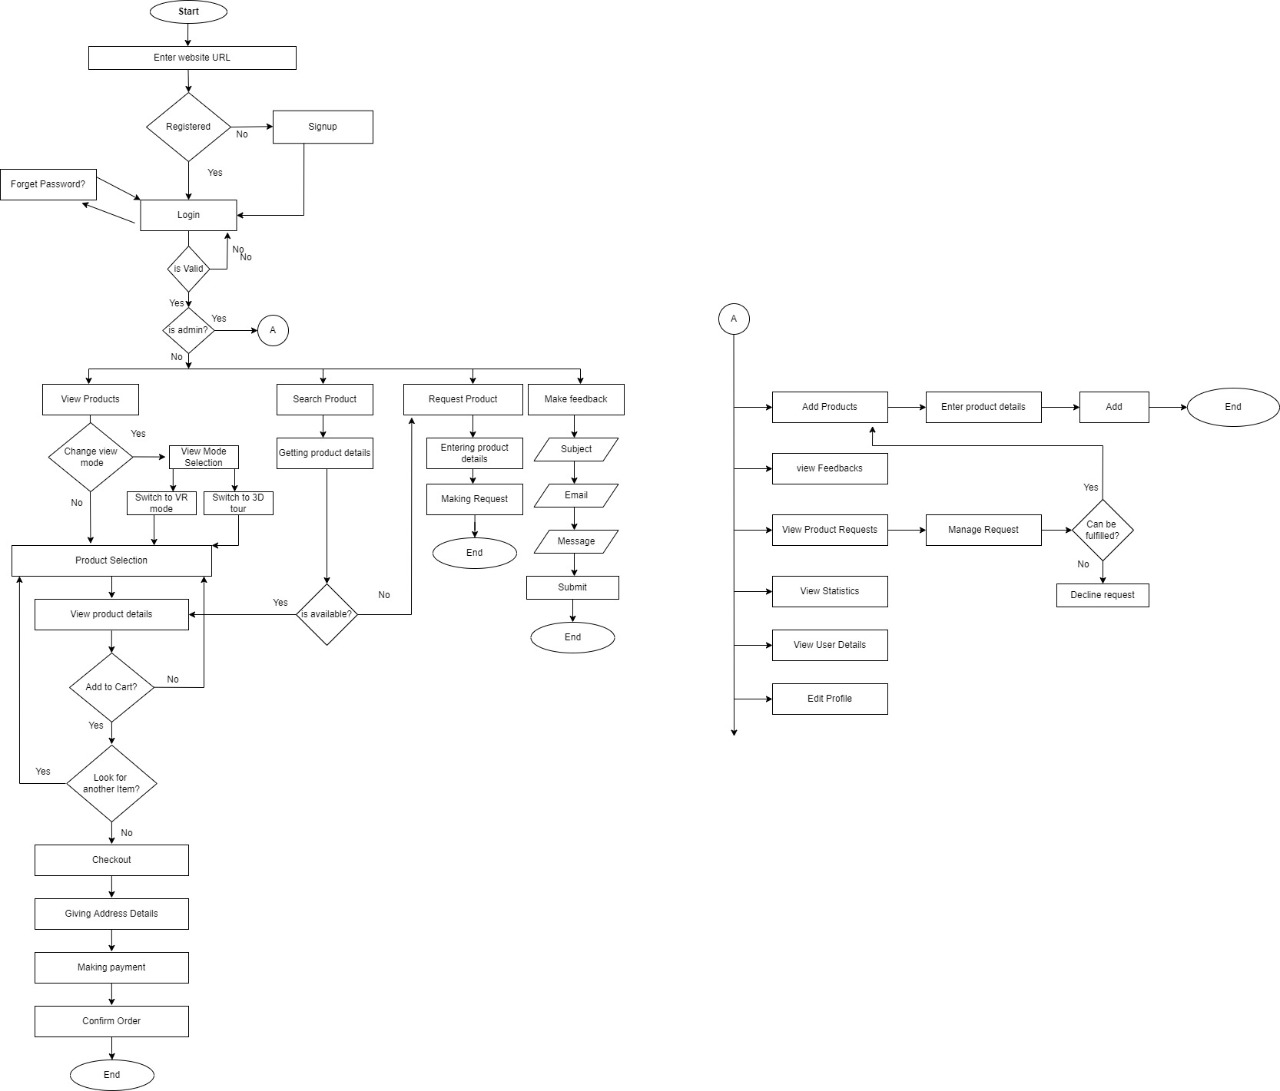
\includegraphics[width=14cm,height=15cm]{Diagrams/FlowChart.jpeg}
    \caption{System’s flowchart diagram}
    \label{fig: System’s flowchart diagram}
    \end{figure}
    \justifying
    This diagram represents the flow of processes. These processes are those which are highly focused during the development of the system. From start to end, the diagram covers all the important steps that are necessary to list there. On the customer side majorly three 3 processes have been listed which are buying a product, requesting a product, and making feedback for the purchased product. Similarly, all processes done by the admin are listed there.

\section{Architectural Diagram}
\subsection{Contextual Diagram}
\begin{figure}[H]
    \centering
    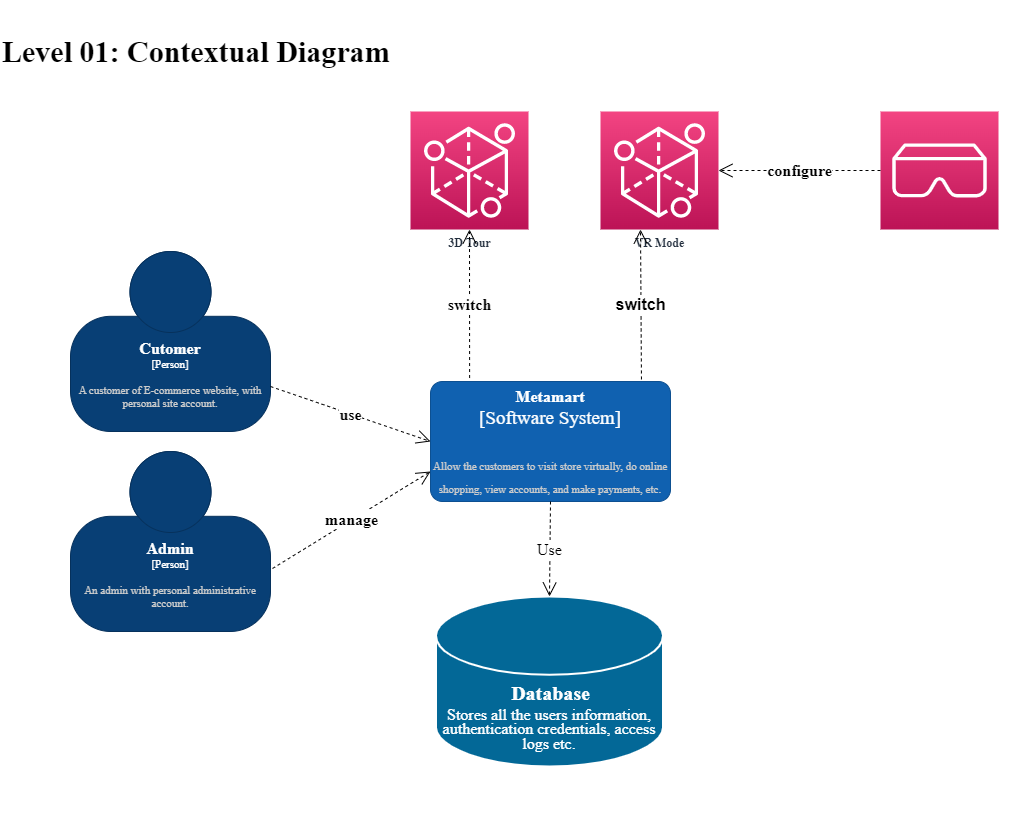
\includegraphics[width=15cm,height=15cm]{Figures/Diagrams/ArchitecturalDiagram/ContextualDiagram.png}
    \caption{Contextual Diagram}
    \label{Contextual Diagram}
\end{figure}
\subsection{Container Diagram}
\begin{figure}[H]
    \centering
    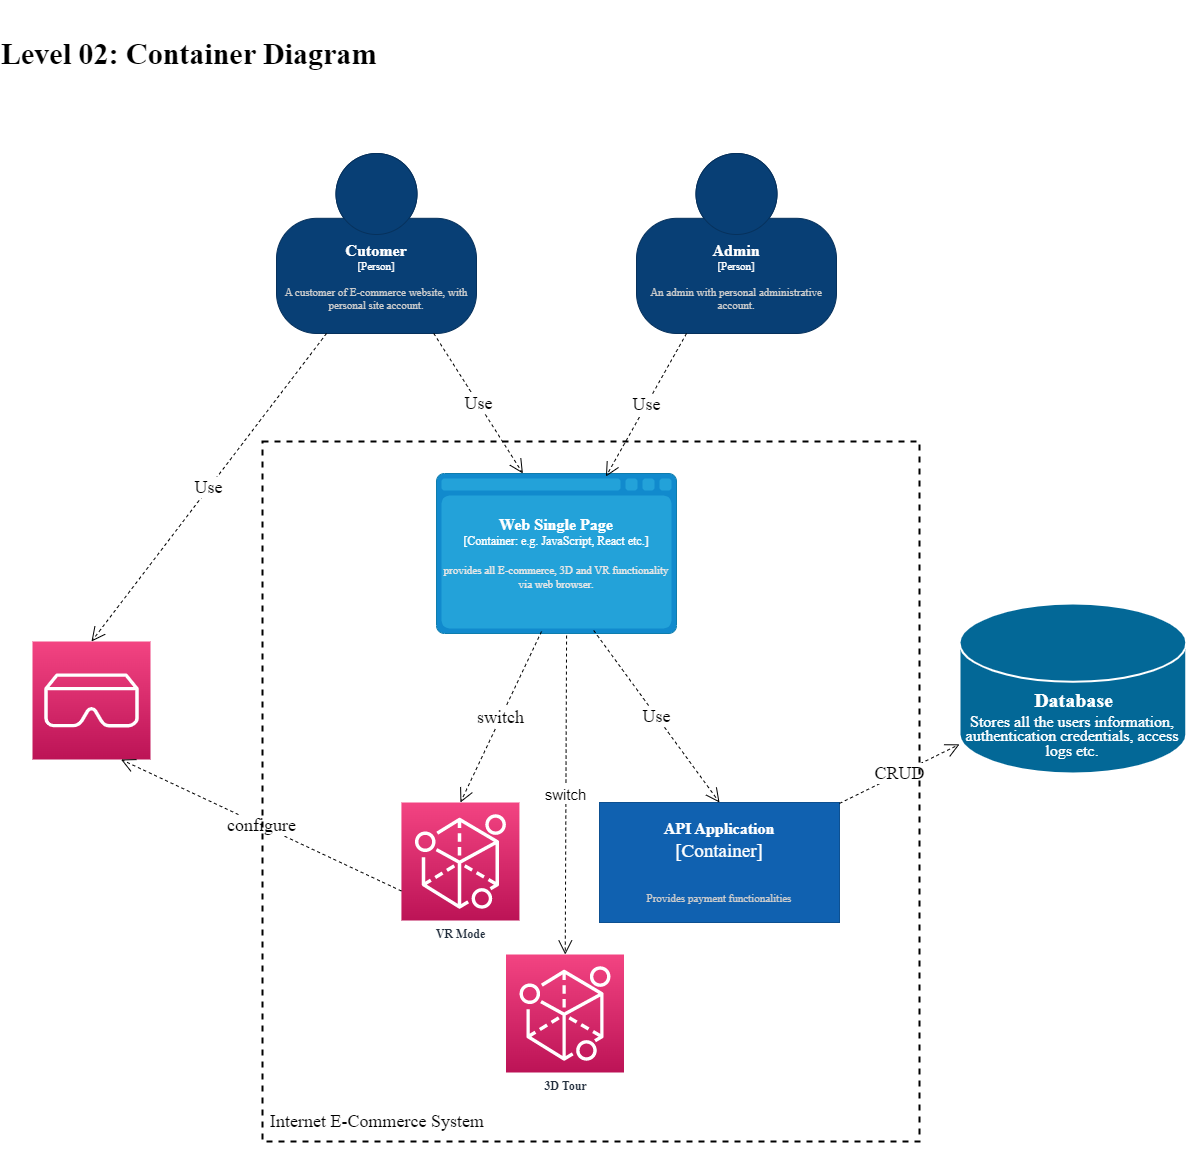
\includegraphics[width=15cm,height=15cm]{Figures/Diagrams/ArchitecturalDiagram/ContainerDiagram.png}
    \caption{Container Diagram}
    \label{Container Diagram}
\end{figure}
\subsection{Component  Diagram}
\begin{figure}[H]
    \centering
    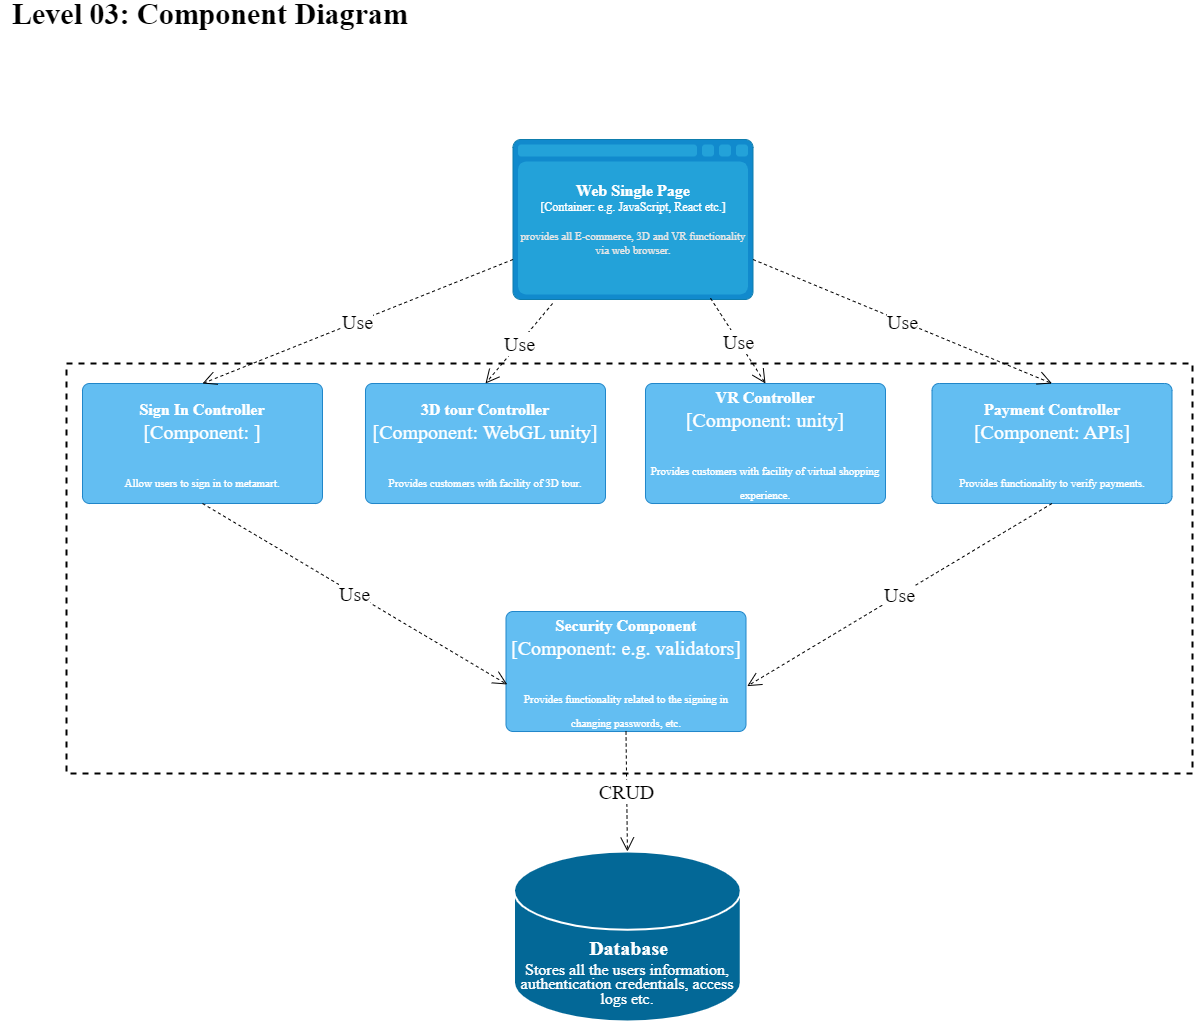
\includegraphics[width=14cm,height=15cm]{Figures/Diagrams/ArchitecturalDiagram/ComponentDiagram.png}
    \caption{Component Diagram}
    \label{Component Diagram}
\end{figure}
\section{Class Diagram}
\begin{figure}[H]
    \centering
    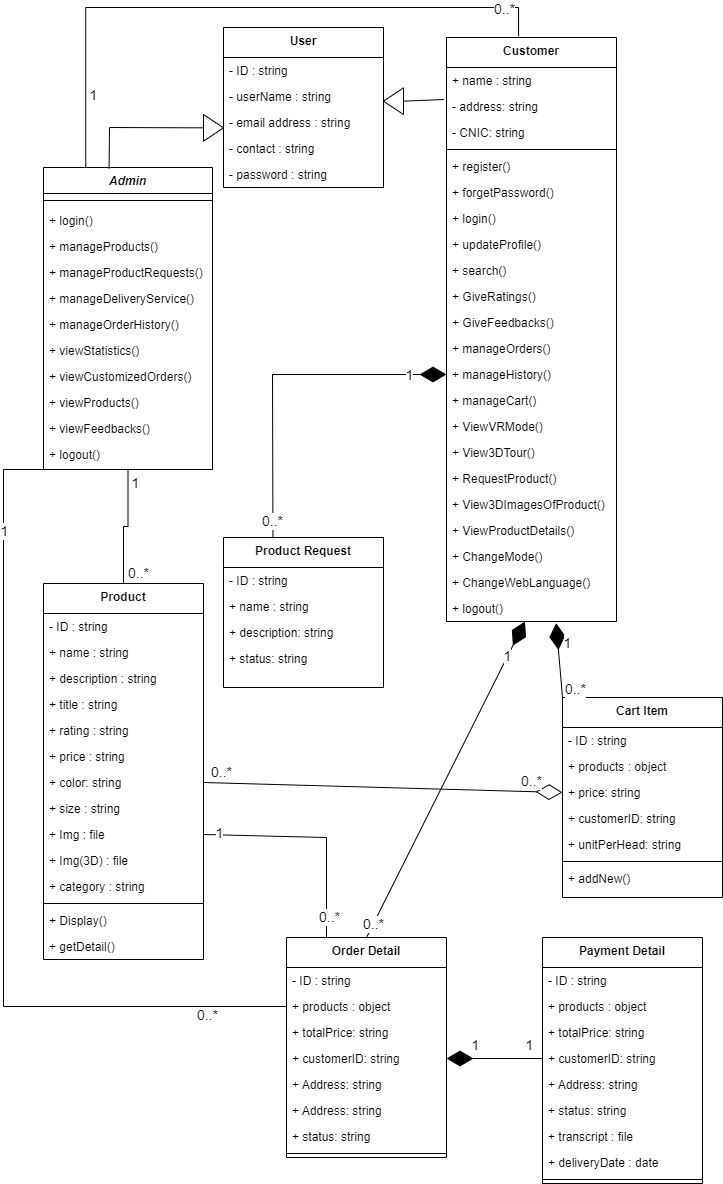
\includegraphics[width=15cm,height=15cm]{Diagrams/ClassDiagram.jpeg}
    \caption{System’s class diagram}
    \label{fig: System’s class diagram}
\end{figure}
\justifying
This class diagram represents the structure of our system. Classes, attributes of those classes, and relationships between classes are shown diagrammatically. Classes are represented by boxes for example user, and customer. Similarly, attributes of a class have been written inside the class box such as the id, username, and email of the class user. Relationships between classes have been represented by arrows between classes. Some arrows represent aggregation/composition.
\section{Entity Relationship Diagram}
\begin{figure}[H]
    \centering
    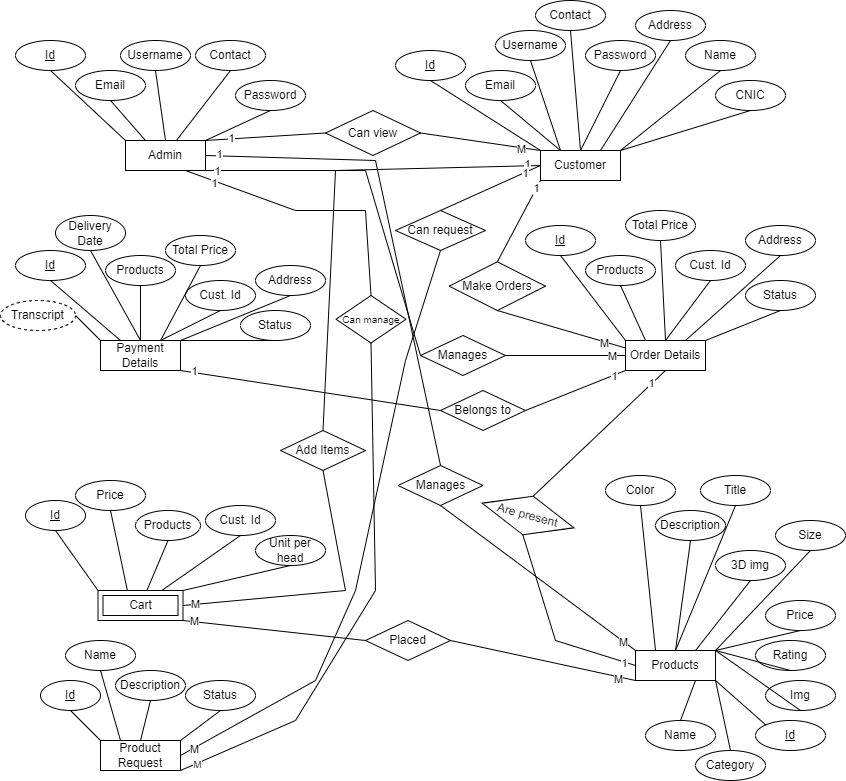
\includegraphics[width=14cm,height=15cm]{Diagrams/erDiagram.jpeg}
    \caption{System’s ERD(Entity Relationship Diagram)}
    \label{fig:System’s ERD(Entity Relationship Diagram)}
   
    \end{figure}
    \justifying
    This class diagram also represents the structure of the system. ERD diagram contains some symbols like rectangles, oval shapes, and lines. Rectangles represent entities which are customer, admin, payment details, cart e.t.c. Oval shapes are attributes of that entity. Similarly, the relationship between two entities is represented by a diamond in an arrow. And types of relationships such as one-to-one, one-to-many, and many-to-many are represented by small numbers near connecting points of the arrow. 


\section{Sequence Diagram}
Following are the sequence diagrams of the customer and admin of the web application that show the control structures between objects.
\subsection{Sequence Diagram for Admin}
\begin{figure}[H]
    \centering
    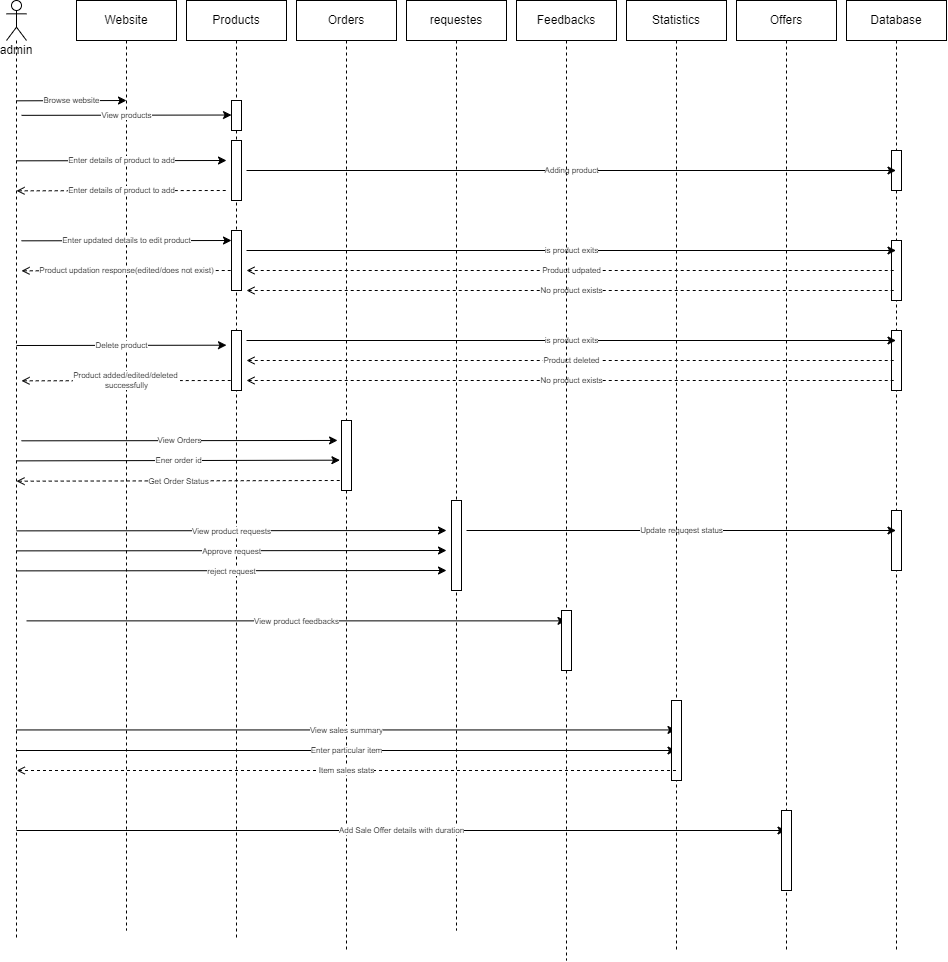
\includegraphics[width=14cm,height=15cm]{Diagrams/Admin_SequenceDiagram.png}
    \caption{System’s Sequence Diagram (Admin)}
    \label{fig: System’s Sequence Diagram (Admin)}

\end{figure}
\justifying
 This diagram shows the whole sequence of steps required by the admin to accomplish different tasks. For example view products, add products, view product requests, give responses to those requests e.t.c. In the diagram rectangles can be seen, these rectangles are modules of the system e.g products, orders, requests, feedback, e.t.c. Where the long bar under every module represents the lifetime for which the user would be interacting with that module. Arrows from user entities to different bars show the user’s purpose of interaction with that module. For example, the admin would interact with the product module to view the product shown in the diagram.
\subsection{Sequence Diagram for Customer}
\begin{figure}[H]
    \centering
    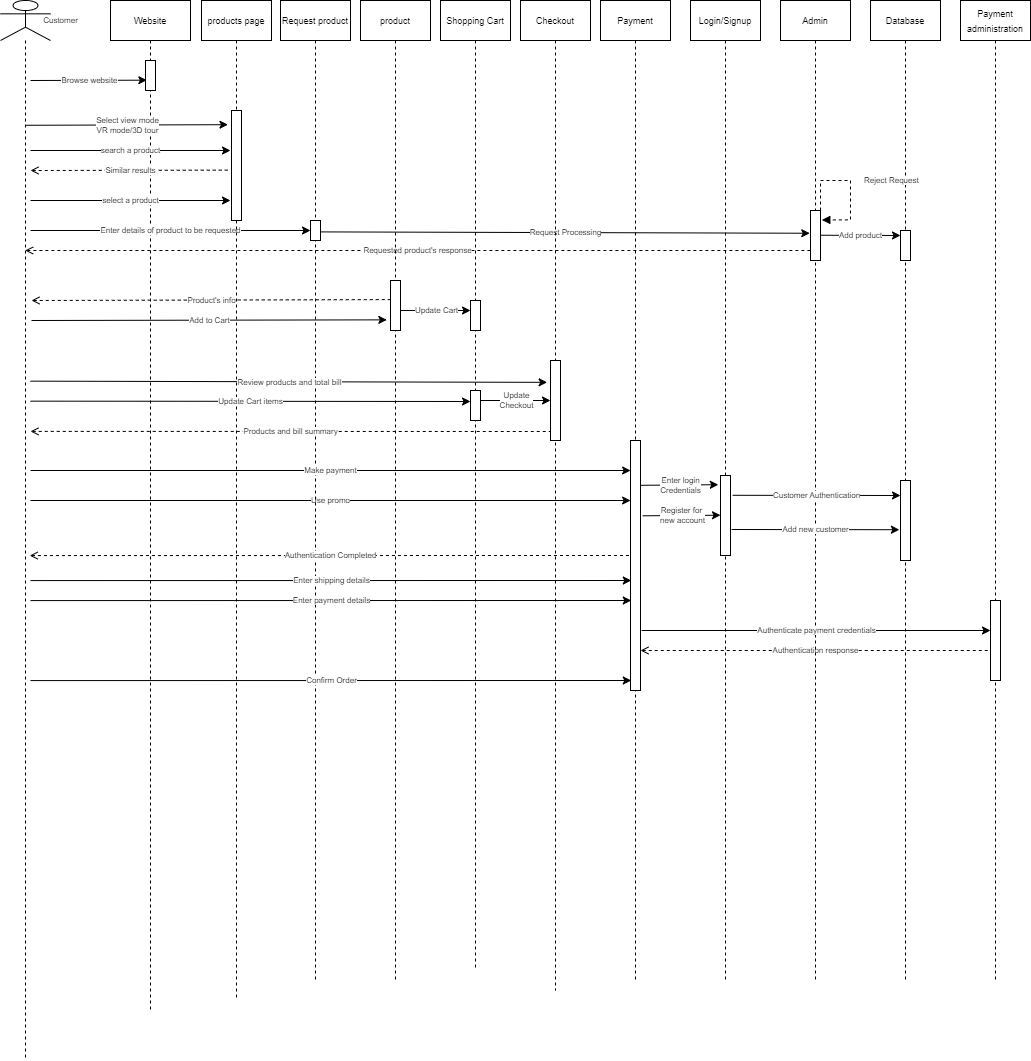
\includegraphics[width=14cm,height=15cm]{Diagrams/Customer_SequenceDiagram.png}
    \caption{System’s Sequence Diagram (Customer)}
    \label{fig: System’s Sequence Diagram (Customer)}
\end{figure}
\justifying
This diagram shows the whole sequence of steps required by customers to accomplish different tasks. For example viewing products, taking orders, making product requests, giving feedback to products e.t.c. In the diagram rectangles can be seen, these rectangles are modules of the system e.g products, shopping cart, payment, e.t.c. Where the long bar under every module represents the lifetime for which the user would be  interacting with that module. Arrows from the user entity to different bars show the user’s purpose of interaction with that module. For example, customers would interact with the product module to view the product shown in the diagram. %
% Chapter 4
\newpage
\begingroup%
\makeatletter%
\let\clearpage\relax% Stop LaTeX from going to a new page; and
\vspace*{\fill}%
\vspace*{\dimexpr-50\p@-\baselineskip}% Remove the initial (default) 50pt gap (plus 1 line)
\chapterfont{\centering}
\chapter{Implementation} % Write in your own chapter title

\vspace*{\fill}%
\endgroup

\newpage
\label{Chapter4}
\lhead{Chapter 4. \emph{Implementation}} % Write in your own chapter title to set the page header


\section{Implementation Details}
The system consists of different modules like an E-commerce website, a 3D tour of a MetaMart store, Virtual reality mode, and fitting size suggestions for customers. These are the main modules of our web application.
The implementation detail of each of the following modules is discussed in detail below.
\section{Rules and assumptions}
Following are rules and cases of assumptions that are assumed to be true while experiencing virtual reality mode working:
\begin{itemize}
    \item The customer has an Oculus VR headset and the configurations/setting for Oculus VR Headset is also done by the customer before going into VR mode.
\end{itemize}
Following are rules and cases of assumptions that are assumed to be true while normally working:
\begin{itemize}
    \item The internet connection is stable.
\end{itemize}
\section{Technology Used}
\subsection{Frontend}
Following are the languages we used in this project:
\begin{itemize}
  \item HTML5
  \item CSS
  \item Bootstrap5
  \item JavaScript
  \item React
  \item NodeJs
  \item Redux
\end{itemize}  
\subsection{Database}
We used  \textbf{MongoDb} database which is one of the popular NoSQL databases.We used mongodb with NodeJs.\\ We also used express as it is also one of the popular backend frameworks for node.
\subsection{API}
Express.Js: It is an open source for node js used to integrate frontend
and backend.

\section{System Requirement}

To be able to use certain hardware or software, the system requirements are required specifications. The configurations for VR headsets are necessary so that the VR headset will work fine and the customer can experience virtual reality mode without any problems. A computer may need certain input and output ports to work with peripheral devices. So as our application requires a VR headset with its configurations on the system, that's why ports should work fine because different cables i.HDMI cables need to be inserted into respective ports.
\subsection{Hardware Requirement}
Following are some of the hardware requirements for this project:
\begin{itemize}
   \item Processor Intel(R)  
    \item Installed RAM 8.00GB
    \item Window 8,10,11
    \item Wireless Adapter(WIFI) or Ethernet connections(LAN)
    \item Oculus VR Headset( For experiencing Virtual reality-based E-commerce store)
\end{itemize}
 
\subsection{Software Requirement}
\begin{itemize}
    \item Software Stack: MERN 
    \item IDE: Visual Studio
    \item Database: MongoDB
    \item Testing API: Postman
\end{itemize}
\section{Tools Used}
A list of all the software that is used to develop and needed to operate the developed module is detailed below:
\begin{table}[H]
    \centering
   \begin{tabular}{ | m{7em} | m{11cm}|}  
  \hline  \textbf{Tools} &  \textbf{Description}  \\  \hline
 \textbf{Make-Human} & MakeHuman is a free and open-source application used for making 3D avatars with custom inputs. Like we just have to set input measurements for the avatars. We can also import and export avatars. Make-Human is developed by a community of programmers.
  \\  \hline
 \textbf{Clo3D} & Clo3D enables you to create virtual 3D samples using best practices and workflow and provides you with basic knowledge of pattern making and digital pattern files. You learn how to instantly modify patterns, fit, and fabrication, with the ability to view changes in colors, prints, and graphics. We can easily make 3D clothes using clo3D.
    \\  \hline
\textbf{ Balsamiq} & Balsamiq Cloud is a web-based user interface design tool for creating wireframes. It can be used to generate digital sketches of your idea or concept for an application or website and to facilitate discussion and understanding before any code is written. You can use Balsamiq to make wireframes. We can make low-fidelity prototypes of our application.
    \\  \hline
 \textbf{ Asana} & Asana is a web and mobile work management platform designed to help teams and organizations organize, track, and manage their tasks or work. 
    \\  \hline
 \textbf{ Github} & GitHub is an online software development platform. It's used for storing, tracking, and collaborating on software projects.GitHub is a great platform for source code sharing and tracking changes in it. With the help of Github, you can easily share your source code with another person.
    \\  \hline
   \textbf{ VS Code} & With VS Code, a free coding editor, you can quickly begin coding.Use it to code in any programming language, without switching editors.
        \\  \hline
    \textbf{Overleaf} & Overleaf is a collaborative cloud-based LaTeX editor used for writing, editing, and publishing scientific documents.
    \\  \hline
    \textbf{Visual Studio} & You can get started coding right away with the help of the free coding editor Visual Studio Code. Visual Studio Code has support for many programming languages, including Python, Java, C++, JavaScript, and many more.
    \\  \hline
    \textbf{  Zoom} & Zoom is a communication Platform. You can use it for users to connect with video, audio, phone, and chat.
       \\  \hline
    \textbf{Postman} & Postman is an API platform for building and using APIs. Postman simplifies each step of the API lifecycle and streamlines collaboration so you can create better APIs—faster.
    \\  \hline
\end{tabular}
    \caption{Tools required for the development of proposed system}
    \label{tab: Tools required for the development of proposed system}
\end{table}
The given table shows the list of different tools that are going to be used for the proposed system’s development. For example, in the first place, there is a tool named “make human”. This tool would be helping out developers in making 3D avatars by giving custom measurements (height, weight, chest size, arm size e.t.c) to the application and getting avatars of that size as output.  Similarly, clo3d will be used for making 3D clothes models to give customers 360-degree exposure. 
\section{3D Jackets View}
\subsection{For Males}
\begin{figure}[H]
    \centering
    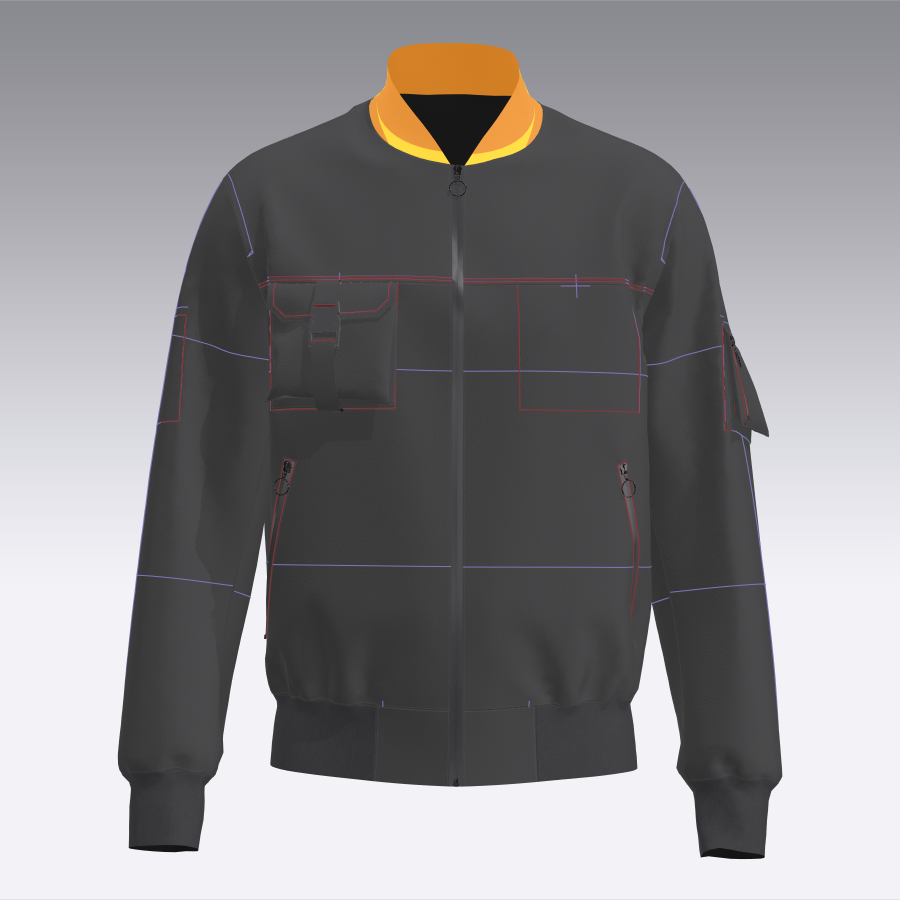
\includegraphics[width=13cm,height=13cm]{Figures/3DJackets/male1.png}
    \caption{3D Model of the grey jacket (Male)}
    \label{fig1:3D Model of the grey jacket (Male)}
   
\end{figure}
\justifying
 A 3D model of a grey color jacket for men made in clo3d. The purpose of this model is to put it on the avatar and render it as a 360-degree rotatable object for customers in 3D environment. This jacket is made by making some patterns and then sewing that patterns according to some measurements.
\begin{figure}[H]
    \centering
    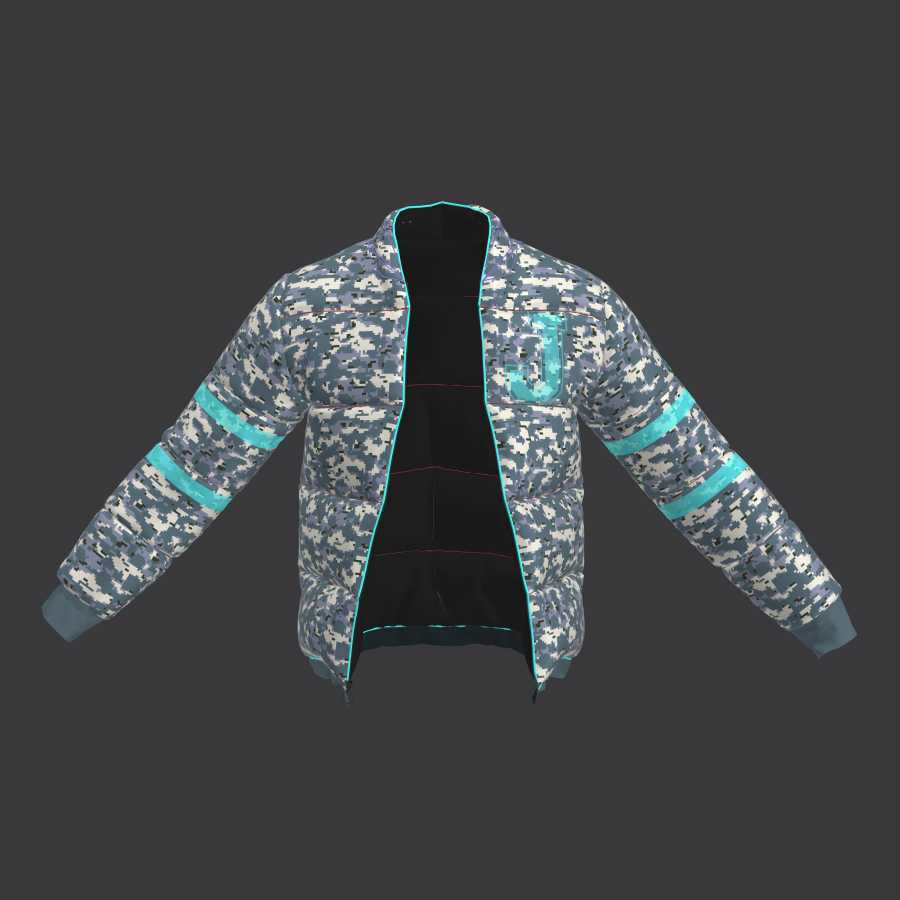
\includegraphics[width=13cm,height=13cm]{Figures/3DJackets/male2.png}
    \caption{3D Model of the jacket (Male)}
    \label{fig2:3D Model of the jacket (Male)}

\end{figure}
\justifying
A 3D model of khaaki color jacket for men made in clo3d. The purpose of this model is to put it on an avatar and render it as a 360-degree rotatable object for customers in a 3D environment. This jacket is made by making some patterns and then sewing that patterns according to some measurements.
\begin{figure}[H]
    \centering
    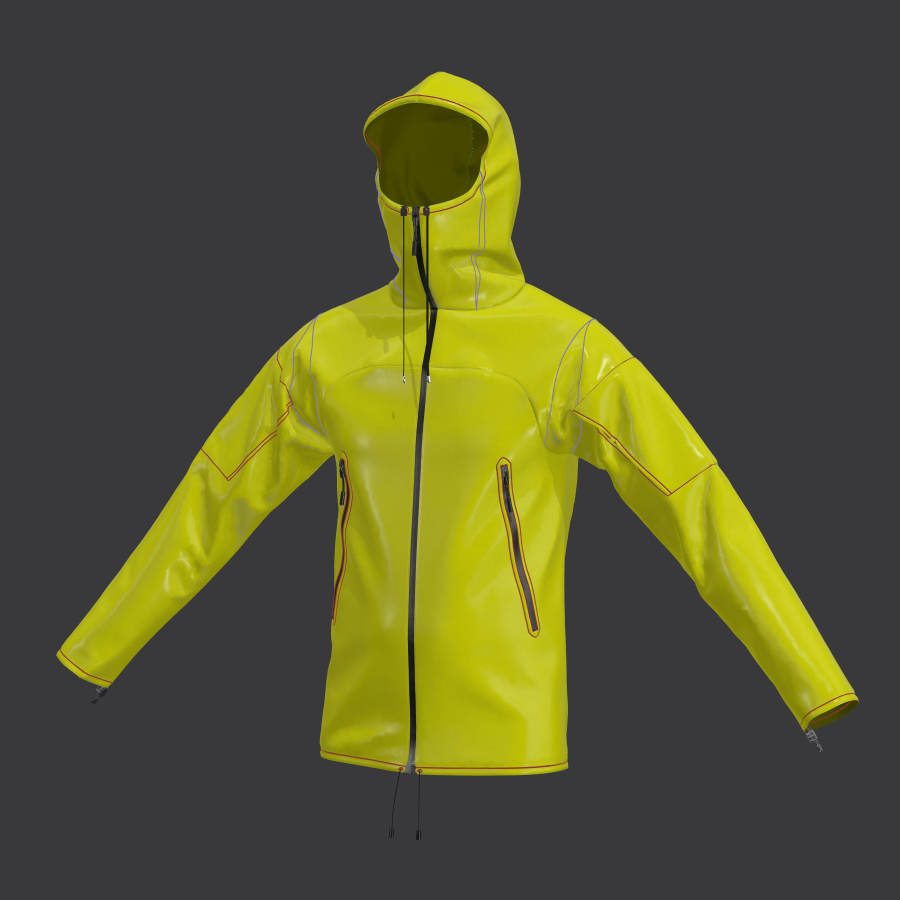
\includegraphics[width=13cm,height=13cm]{Figures/3DJackets/male3.png}
    \caption{3D Model of the yellow jacket (Male)}
    \label{fig3:3D Model of the yellow jacket (Male)}
\end{figure}
\justifying
A 3D model of a yellow color jacket for men made in clo3d. The purpose of this model is to put it on the avatar and render it as a 360-degree rotatable object for customers in a 3D environment. This jacket is made by making some patterns and then sewing that patterns according to some measurements.
\begin{figure}[H]
    \centering
    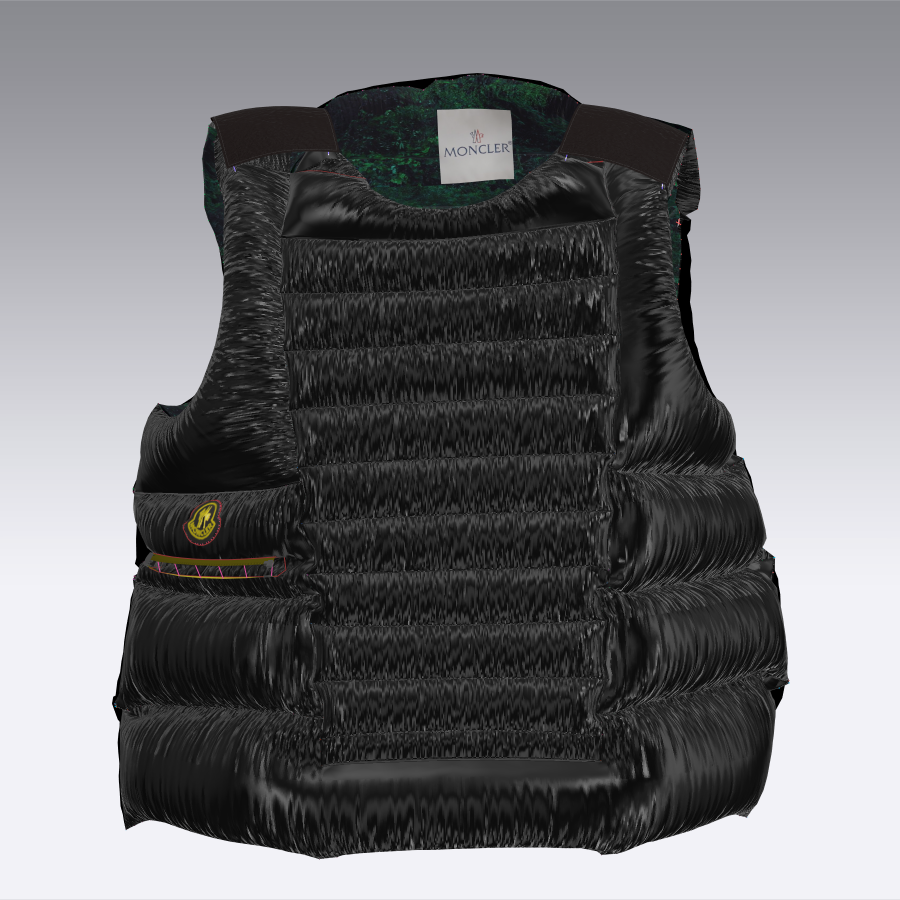
\includegraphics[width=13cm,height=13cm]{Figures/3DJackets/male4.png}
    \caption{3D Model of sleeveless black puffer jacket (Male)}
    \label{fig4:3D Model of sleeveless black puffer jacket (Male)}
  
\end{figure}
\justifying
A 3D model of black color puffer jacket for men made in clo3d. The purpose of this model is to put it on the avatar and render it as a 360-degree rotatable object for customers in a 3D environment. This jacket is made by making some patterns and then sewing that patterns according to some measurements.
\begin{figure}[H]
    \centering
    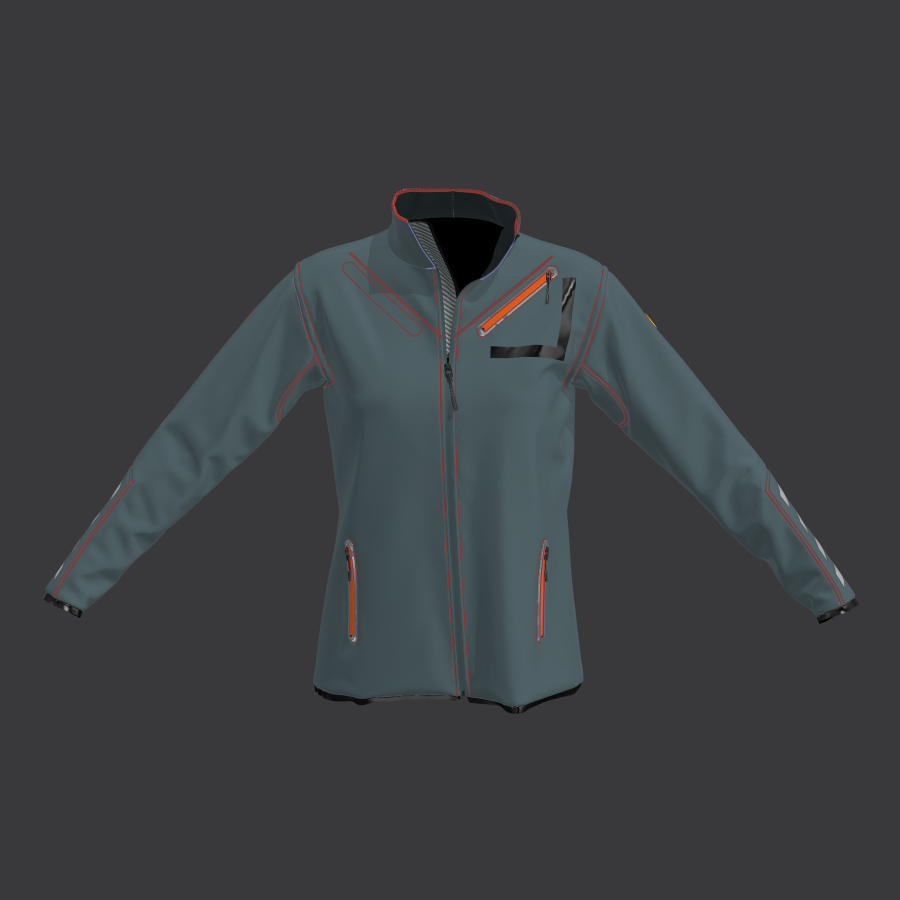
\includegraphics[width=15cm,height=15cm]{Figures/3DJackets/male5.png}
    \caption{3D Model of the jacket (Male)}
    \label{fig5:3D Model of the jacket (Male)}
\end{figure}
\justifying
A 3D model of a jacket for men made in clo3d. The purpose of this model is to put it on the avatar and render it as a 360-degree rotatable object for customers in a 3D environment. This jacket is made by making some patterns and then sewing that patterns according to some measurements.
\subsection{For Females}
\begin{figure}[H]
    \centering
    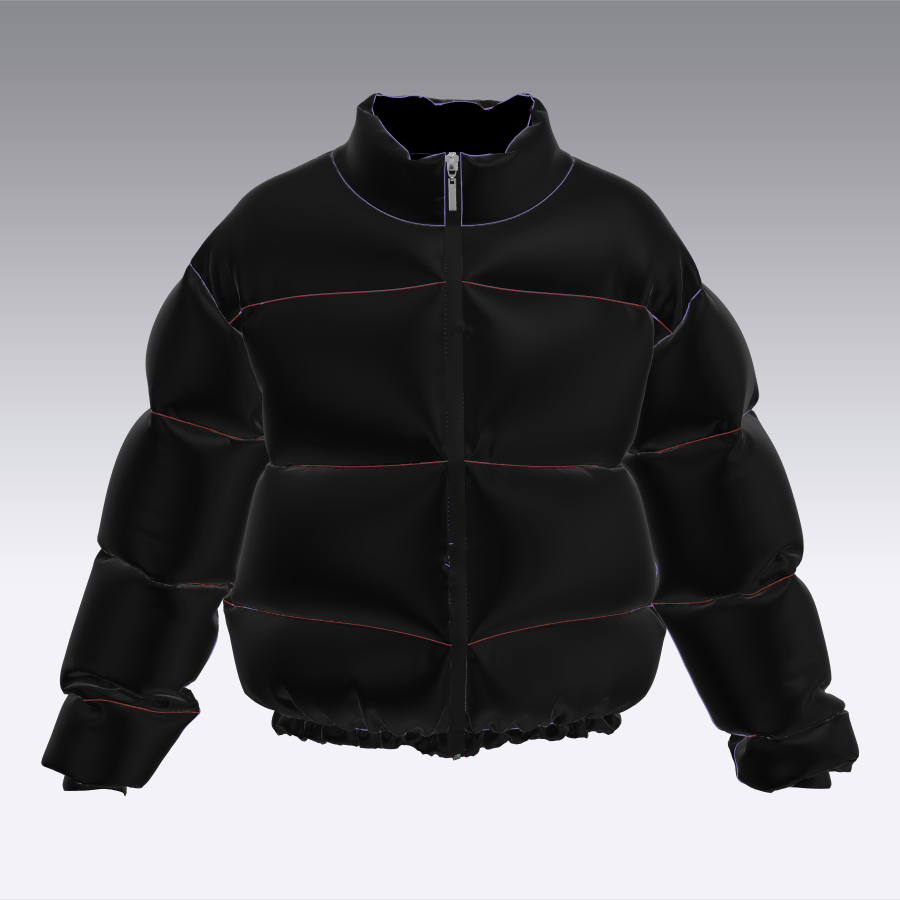
\includegraphics[width=13cm,height=12cm]{Figures/3DJackets/female1.png}
    \caption{3D Model of puffer jacket (Female)}
    \label{fig1:3D Model of puffer jacket (Female)}
\end{figure}
\justifying
A 3D model of a black color jacket for females. The purpose of this model is to put it on the avatar and render it as a 360-degree rotatable object for customers in a 3D environment. This jacket is made by making some patterns and then sewing that patterns according to some measurements.
\begin{figure}[H]
    \centering
    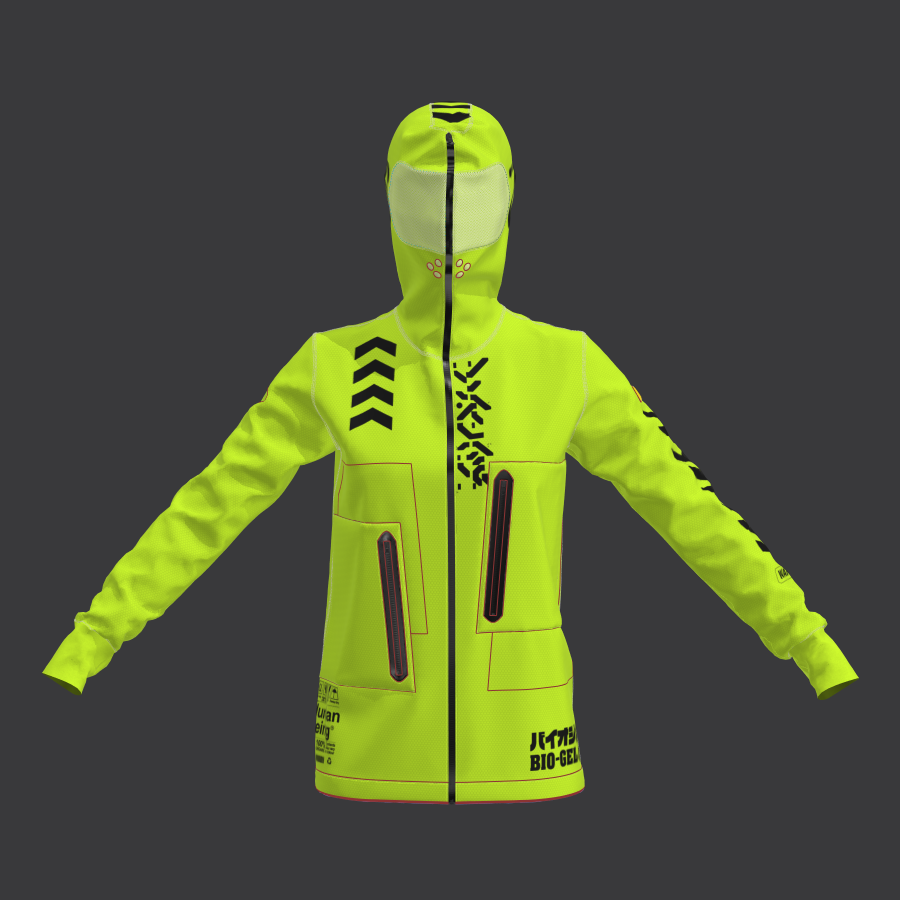
\includegraphics[width=13cm,height=12cm]{Figures/3DJackets/female2.png}
    \caption{3D Model of the stylish designed jacket (Female)}
    \label{3D Model of the stylish designed jacket (Female)}

\end{figure}
A 3D model of a well-designed jacket for females. The purpose of this model is to put it on the avatar and render it as a 360-degree rotatable object for customers in a 3D environment. This jacket is made by making some patterns and then sewing that patterns according to some measurements.
\begin{figure}[H]
    \centering
    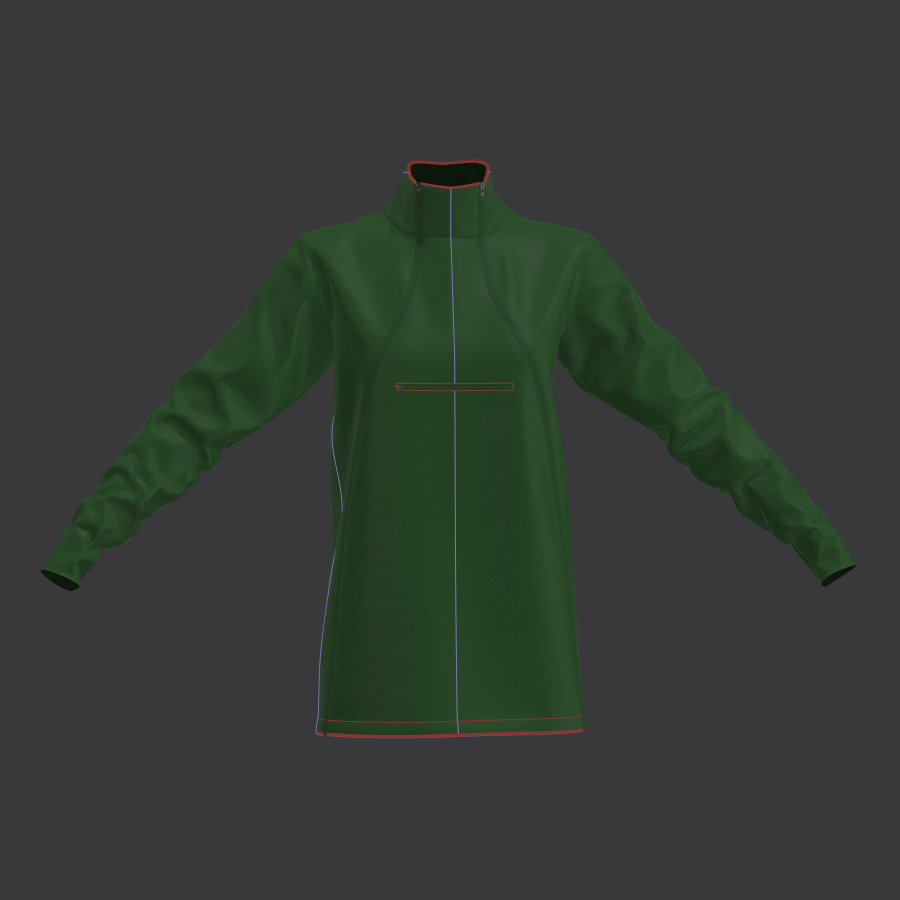
\includegraphics[width=13cm,height=12cm]{Figures/3DJackets/female3.png}
    \caption{3D Model of the green leather jacket (Female)}
    \label{3D Model of the green leather jacket (Female)}
   
\end{figure}
A 3D model of a well-designed leather jacket for females. The purpose of this model is to put it on the avatar and render it as a 360-degree rotatable object for customers in the 3D environment. This jacket is made by making some patterns and then sewing that patterns according to some measurements.
\begin{figure}[H]
    \centering
    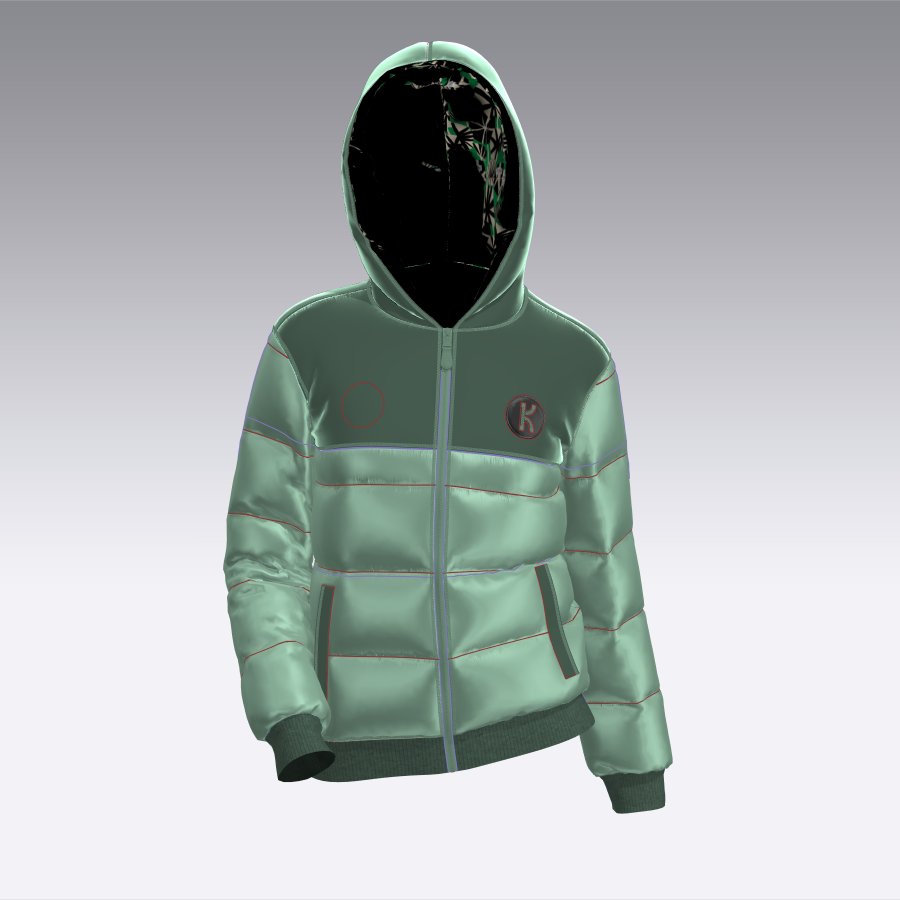
\includegraphics[width=13cm,height=12cm]{Figures/3DJackets/female4.png}
    \caption{3D Model of beautifully designed puffer jacket (Female)}
    \label{3D Model of beautifully designed puffer jacket (Female)}
  
\end{figure}
\justifying
A 3D model of a well-designed puffer jacket for females. The purpose of this model is to put it on the avatar and render it as a 360-degree rotatable object for customers in a 3D environment. This jacket is made by making some patterns and then sewing that patterns according to some measurements.
\section{3D Avatars wearing Jackets View}
\subsection{For Males}
\begin{figure}[H]
    \centering
    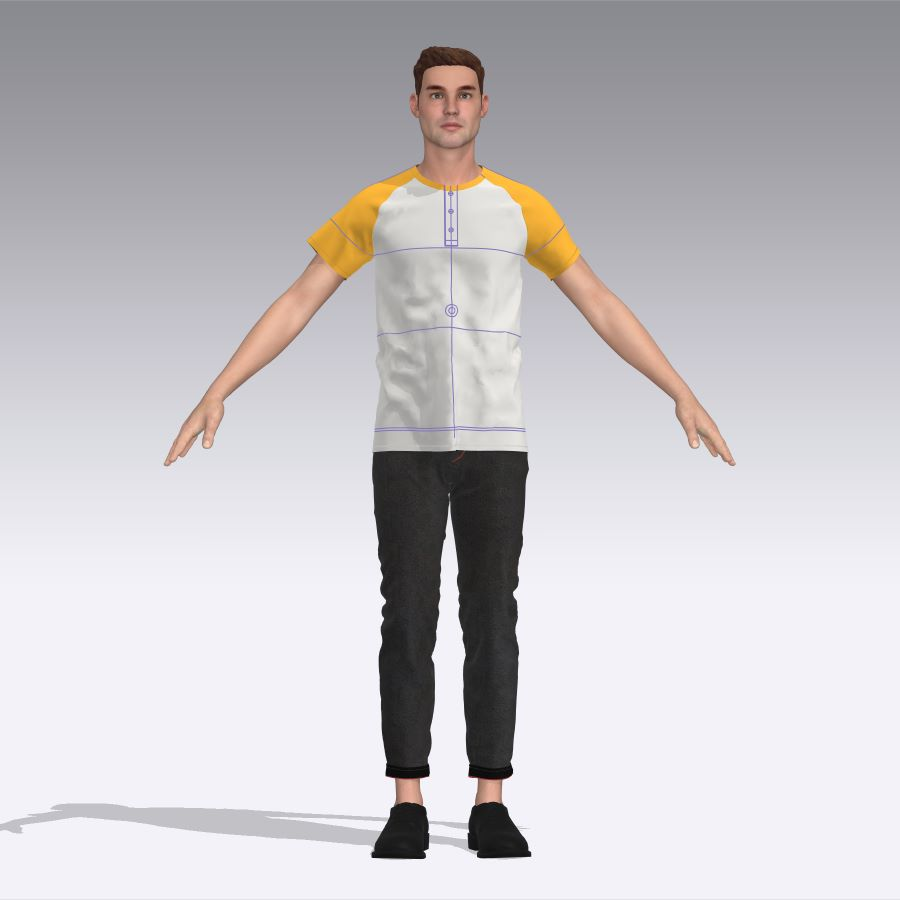
\includegraphics[width=13cm,height=12cm]{Figures/3DAvatars/male1.jpeg}
    \caption{Male Avatar wearing t-shirt and pants}
    \label{Male Avatar wearing t-shirt and pants}
   
\end{figure}
	Avatar is a 3D rotatable object made in make humans with customer inputs. It would be used for displaying 3D clothes to the customer just like in the real world there are statues for displaying clothes and customers can move around that statue for checking cloth.  
\begin{figure}[H]
    \centering
    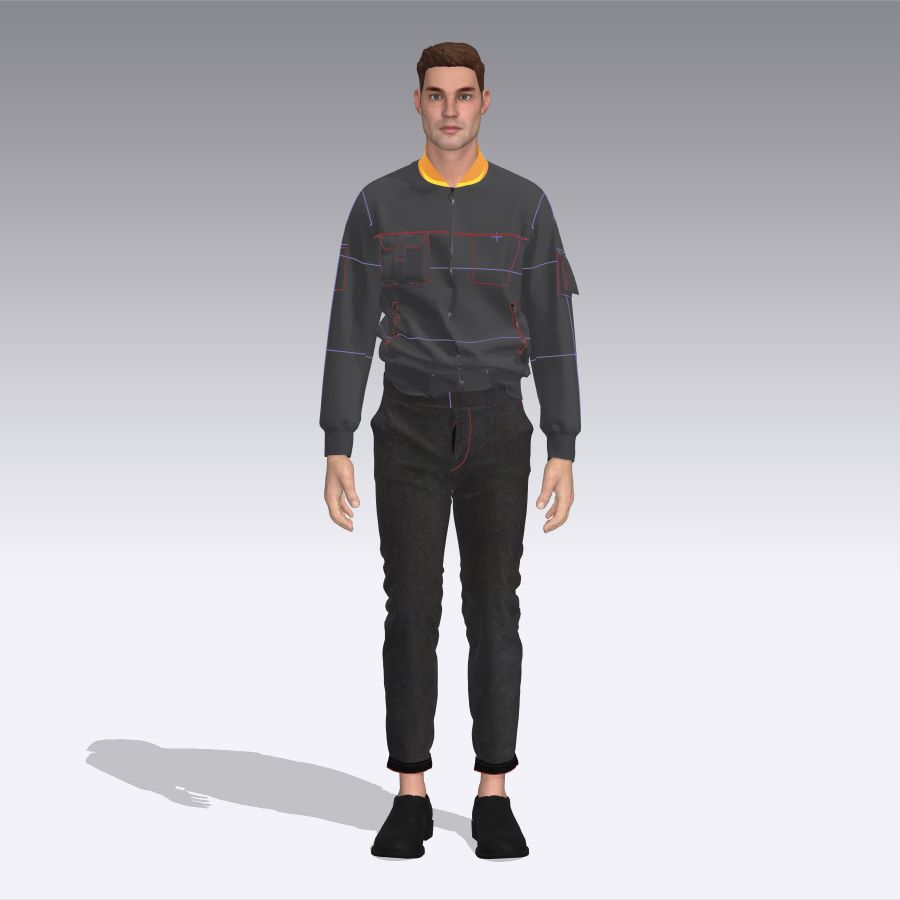
\includegraphics[width=12cm,height=10cm]{Figures/3DAvatars/male2.jpeg}
    \caption{Male Avatar wearing jacket and pants}
    \label{Male Avatar wearing jacket and pants}
 
\end{figure}
Avatar is a 3D rotatable object made in make humans with customer inputs. It would be used for displaying 3D clothes to the customer just like in the real world there are statues for displaying clothes and customers can move around that statue for checking cloth.  
\begin{figure}[H]
    \centering
    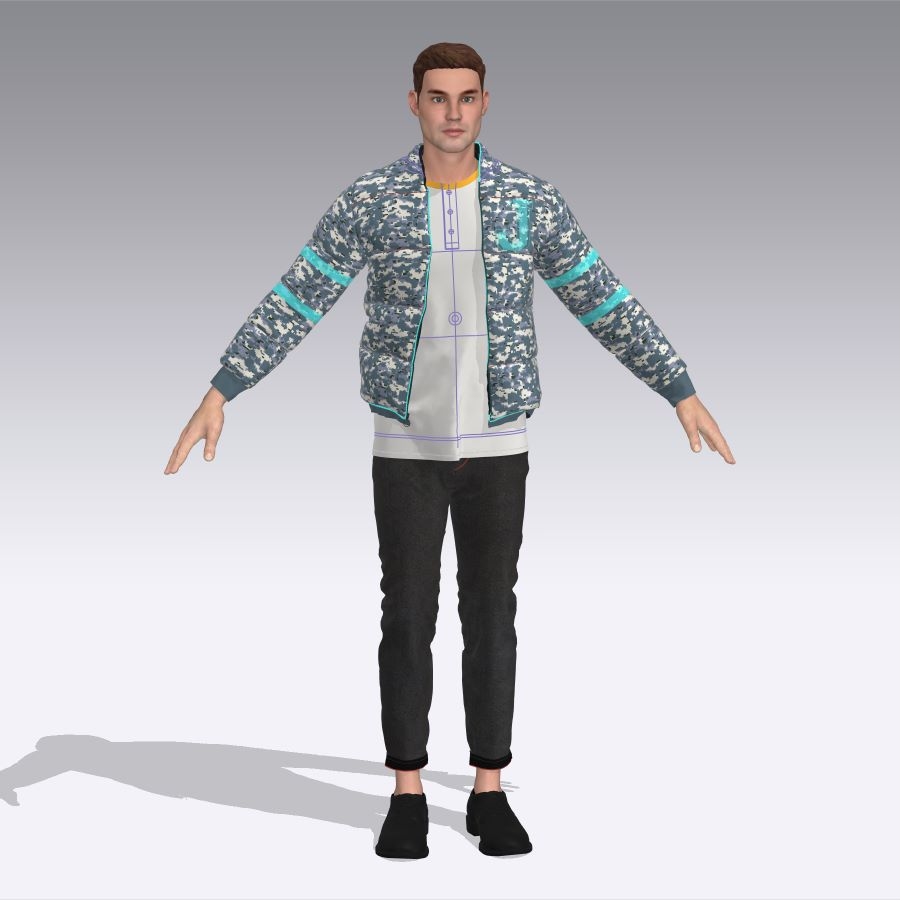
\includegraphics[width=13cm,height=10cm]{Figures/3DAvatars/male3.jpeg}
    \caption{Asian Male Avatar wearing jacket and pants}
    \label{Male Avatar wearing jacket and pants}
    
\end{figure}
Avatar is a 3D rotatable object made in make humans with customer inputs. It would be used for displaying 3D clothes to the customer just like in the real world there are statues for displaying clothes and customers can move around that statue for checking cloth.  
\begin{figure}[H]
    \centering
    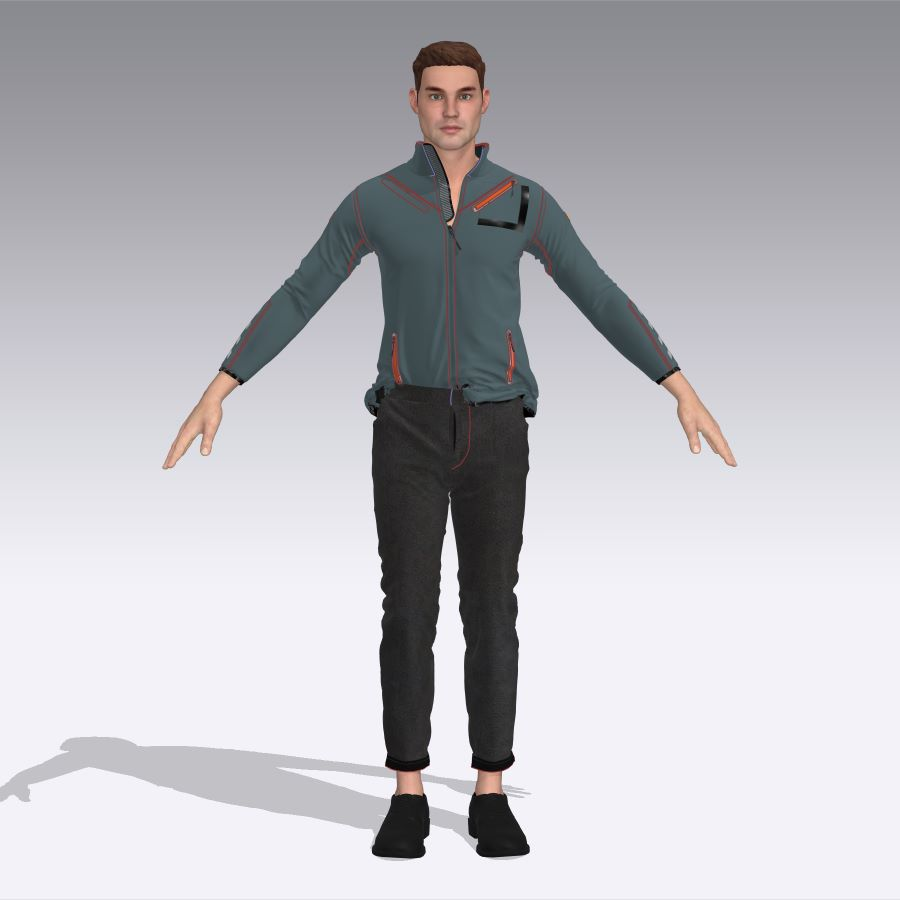
\includegraphics[width=13cm,height=10cm]{Figures/3DAvatars/male4.jpeg}
    \caption{Male Avatar wearing jacket and black pants}
    \label{Male Avatar wearing jacket and black pants}

\end{figure}
\justifying
	Avatar is a 3D rotatable object made in make humans with customer inputs. It would be used for displaying of 3D clothes to the customer just like in the real world there are statues for displaying clothes and customers can move around that statue for checking cloth.  
\subsection{For Females}
\begin{figure}[H]
    \centering
    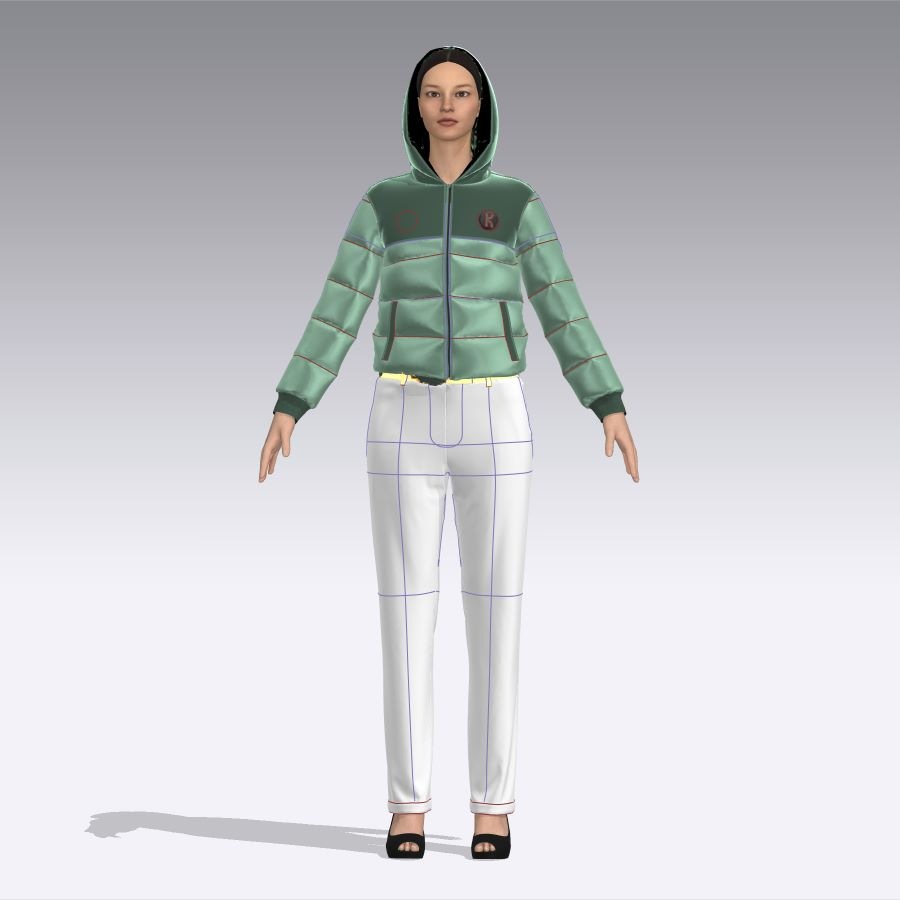
\includegraphics[width=12cm,height=10cm]{Figures/3DAvatars/female1.jpeg}
    \caption{Female Avatar wearing a puffer jacket and white pants}
    \label{Female Avatar wearing a puffer jacket and white pants}
    
\end{figure}
\justifying
Avatar is a 3D rotatable object made in make humans with customer inputs. It would be used for displaying 3D clothes to the customer just like in the real world there are statues for displaying clothes and customers can move around that statue for checking cloth.  


\begin{figure}[H]
    \centering
    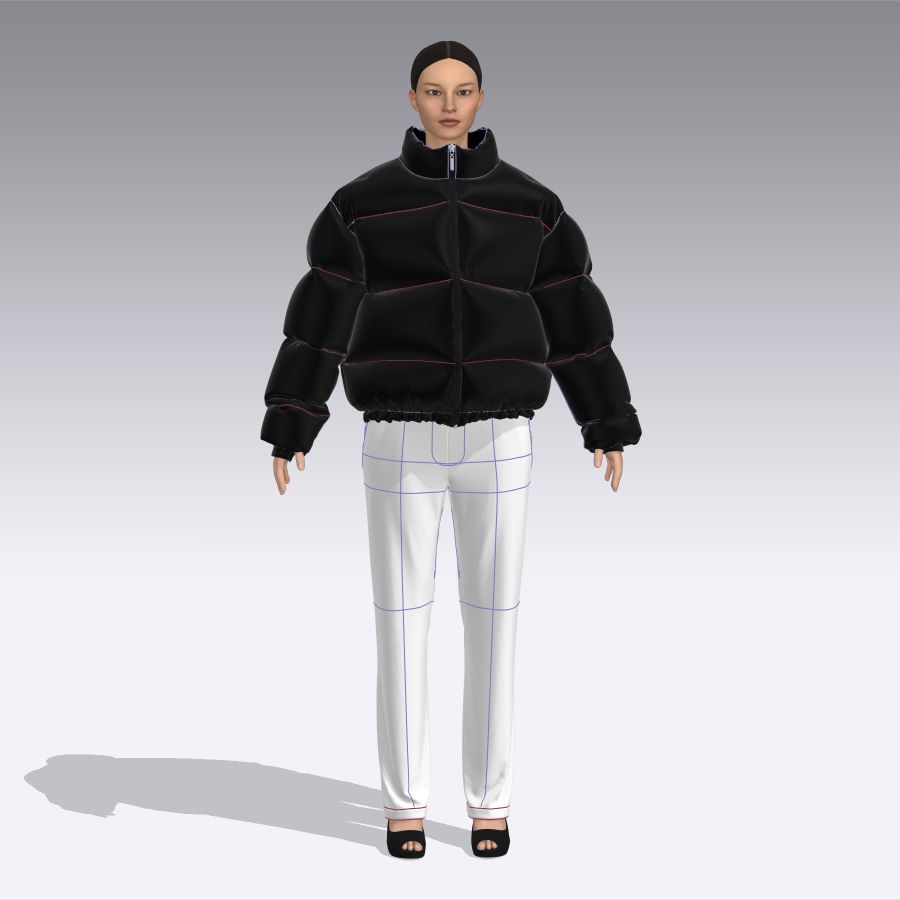
\includegraphics[width=13cm,height=12cm]{Figures/3DAvatars/female2.jpeg}
    \caption{Female Avatar wearing a stylish black puffer jacket and white pants}
    \label{fig2:Stylish designed 3D jacket for females.In this image, you can see the female avatar wearing the jacket. This is the front view.}
\end{figure}
\justifying
	Avatar is a 3D rotatable object made in make humans with customer inputs. It would be used for displaying 3D clothes to the customer just like in the real world there are statues for displaying clothes and customers can move around that statue for checking cloth.  
\section{Unity Environment View}
\subsection{Virtual city in Meta verse}
\begin{figure}[H]
    \centering
    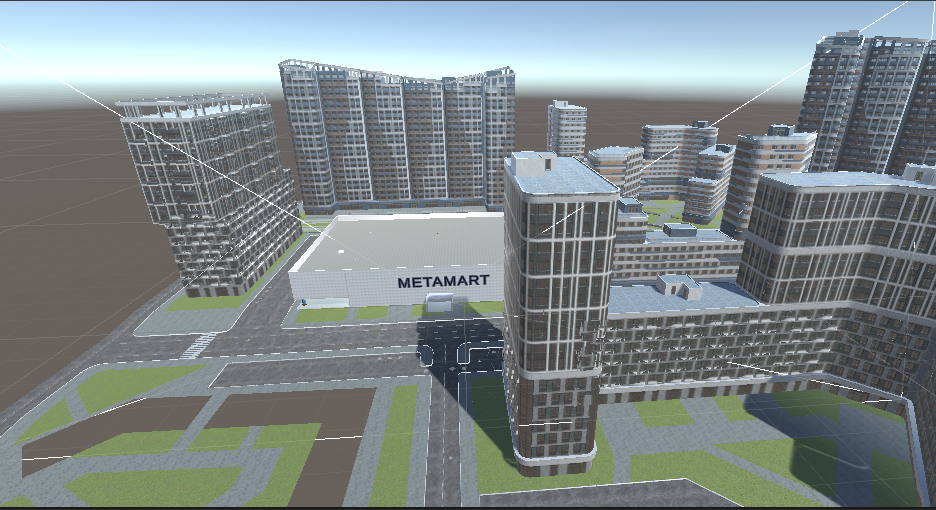
\includegraphics[width=12cm,height=10cm]{Figures/Environment/City.png}
    \caption{Virtual store outer view}
    \label{fig: Virtual store outer view}
\end{figure}
  The virtual store's outer view is shown in this image.
\subsection{Entrance of MetaMart}
\begin{figure}[H]
    \centering
    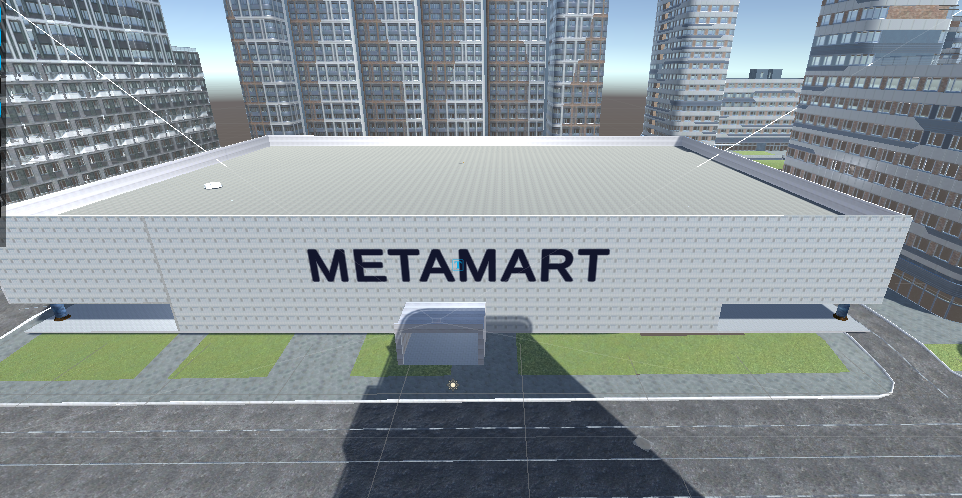
\includegraphics[width=12cm,height=10cm]{Figures/Environment/Entrance.png}
    \caption{Entrance of MetaMart}
    \label{fig: Entrance of MetaMart}
\end{figure}
\justifying
  Entrance of MetaMart through which the customer will enter in the MetaMart.
\subsection{Inside View of MetaMart}
\begin{figure}[H]
    \centering
    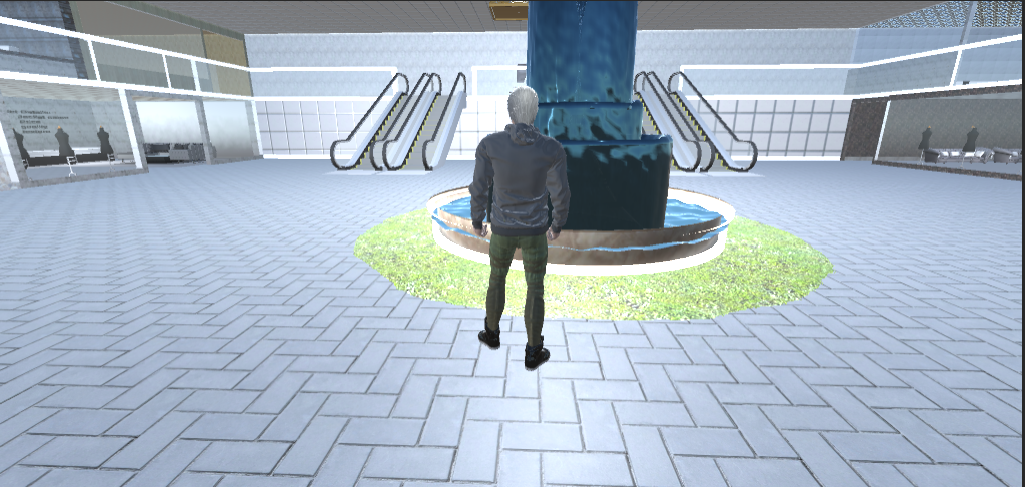
\includegraphics[width=12cm,height=10cm]{Figures/Environment/insideview.png}
    \caption{Inside view of MetaMart}
    \label{fig: Entrance of MetaMart}
    
\end{figure}
The front view of shops in MetaMart is in this image is shown.
\subsection{Inside View of MetaMart}
\begin{figure}[H]
    \centering
    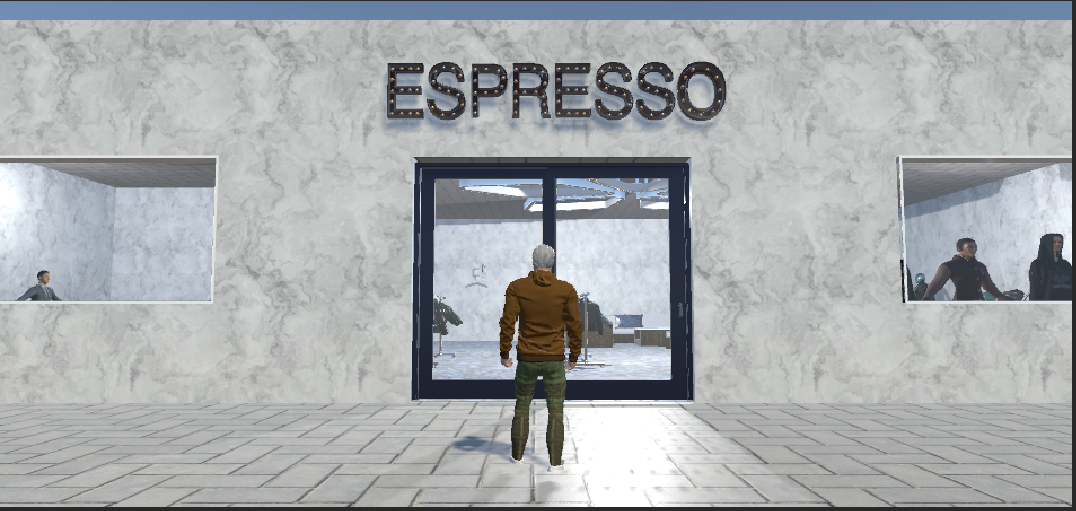
\includegraphics[width=13cm,height=12cm]{Figures/Environment/shop.png}
    \caption{Shop View of MetaMart}
    \label{fig:Shop View of MetaMart}
\end{figure}
The front view of shop in MetaMart in this image is shown.
\subsection{Inside Shop view in MetaMart}
\begin{figure}[H]
    \centering
    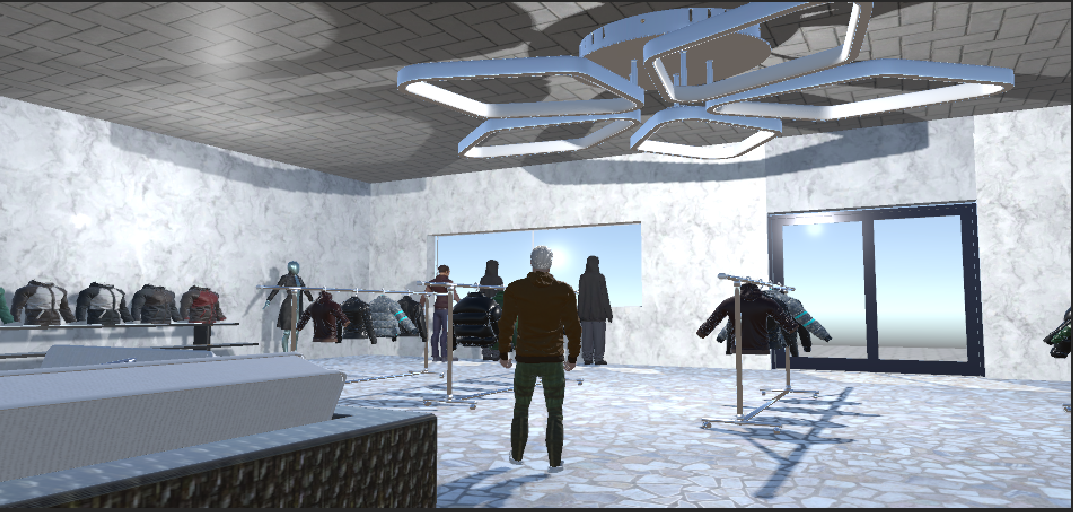
\includegraphics[width=13cm,height=12cm]{Figures/Environment/insideshop.png}
    \caption{Inside View of MetaMart}
    \label{fig:Inside View of MetaMart}
\end{figure}
  Inside View of MetaMart like when the customer enters the shop in MetaMart this view will be shown to the customer.
  \begin{figure}[H]
    \centering
    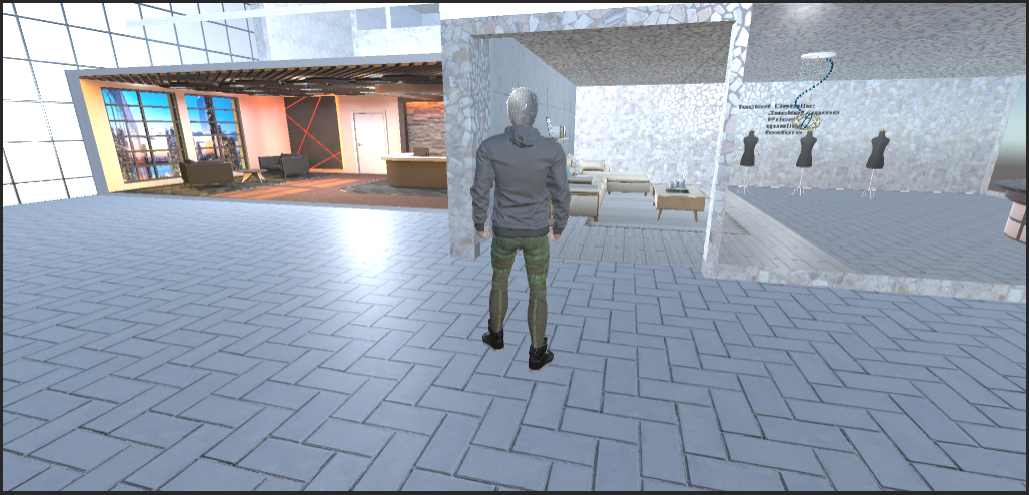
\includegraphics[width=13cm,height=12cm]{Figures/Environment/insideview22.png}
    \caption{Inside View of MetaMart (2)}
    \label{fig:Inside View of MetaMart(2)}
\end{figure}
  Inside View of MetaMart like when the customer enters the shop in MetaMart this view will be shown to the customer.
\begin{figure}[H]
    \centering
    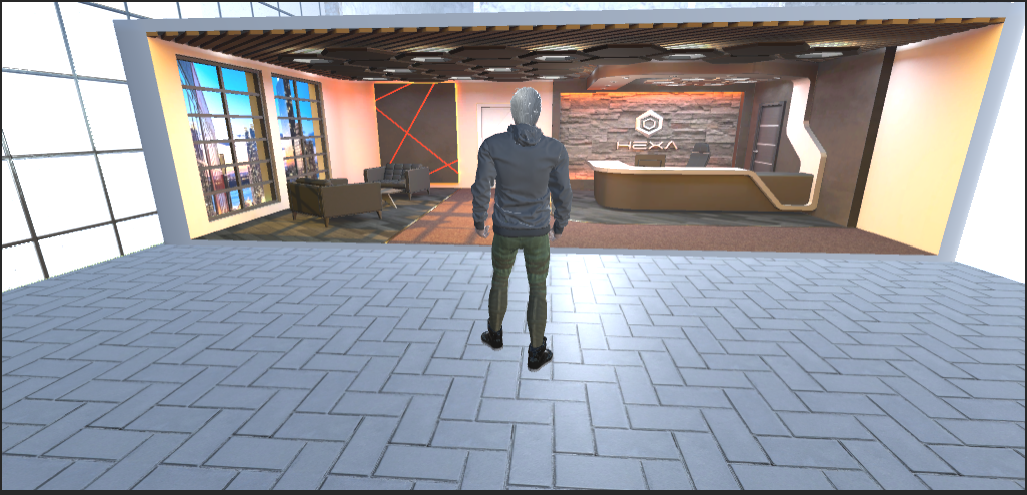
\includegraphics[width=15cm,height=15cm]{Figures/Environment/insidevie2.png}
    \caption{Inside View of MetaMart(2)}
    \label{fig: Entrance of MetaMart}
\end{figure}
\justifying
  There are different shops inside the MetaMart like when the customer enters in the MetaMart this is the first shop in which there will be different outerwears for men.
\begin{figure}[H]
    \centering
    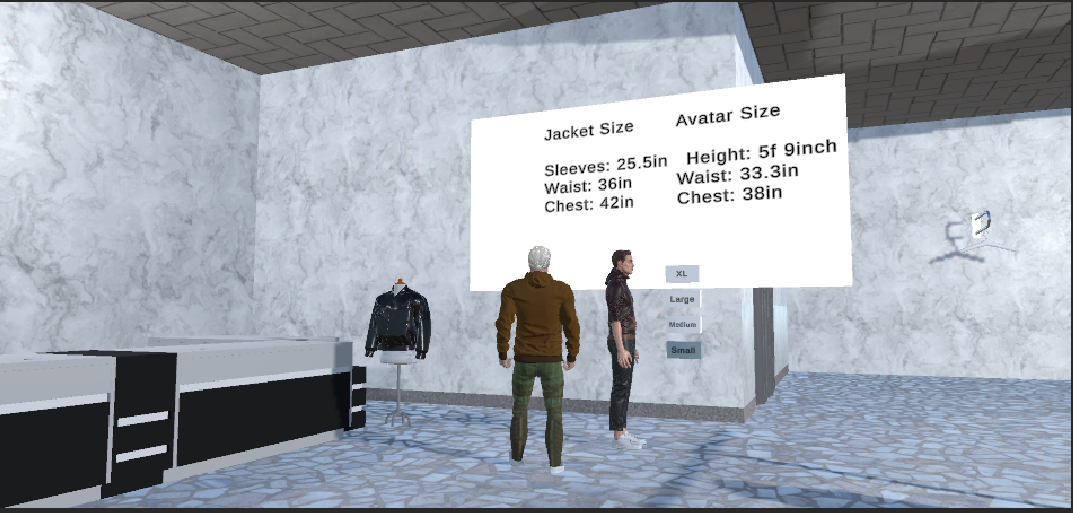
\includegraphics[width=15cm,height=15cm]{Figures/Environment/products.png}
    \caption{Jacket details shown to the customer}
    \label{fig:Product Details showing}
\end{figure}
\justifying
When a customer approaches a product, its details will be displayed to the user, just like this.
\section{Virtual Reality-based E-commerce Web Application Interface}
\subsection{Admin Section}
Following are some of the screenshots of the Admin section:
\subsubsection{Sign-In Screen}
\begin{figure}[H]
    \centering
    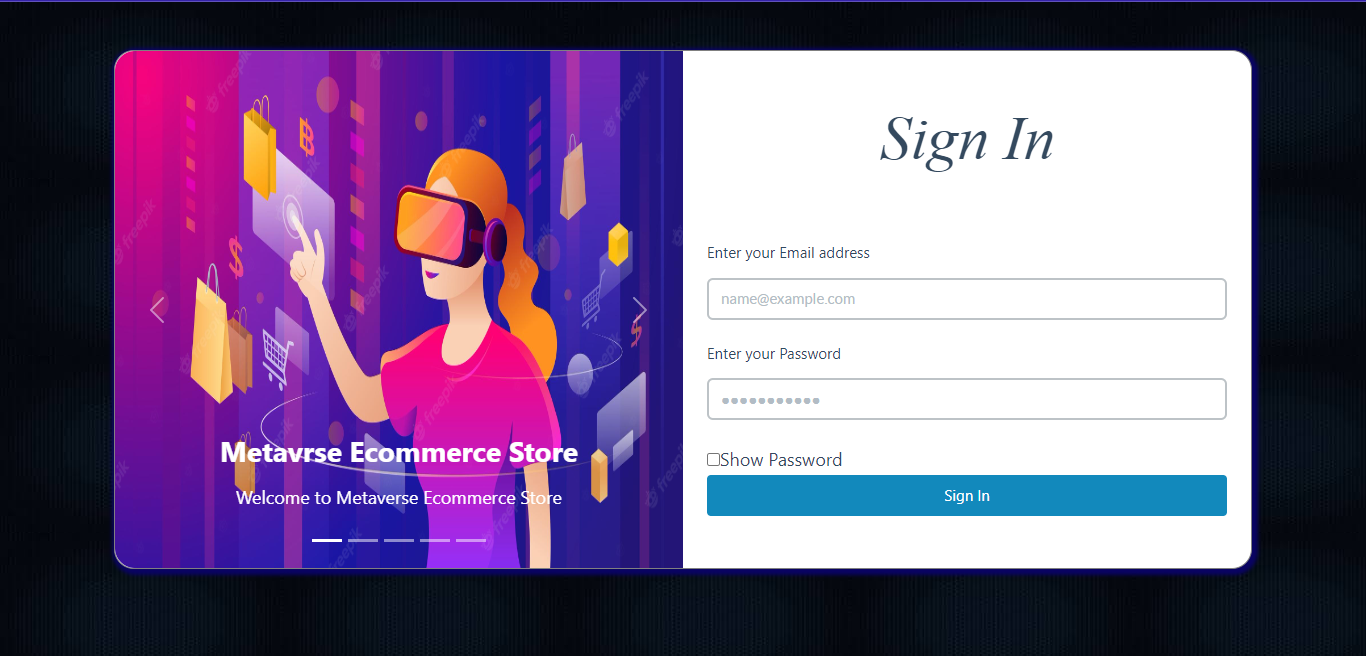
\includegraphics[width=15cm,height=12cm]{Figures/Diagrams/SignIn.PNG}
    \caption{System’s sign-in screen (Admin)}
    \label{System’s sign-in screen (Admin)}
    It is the sign In page for the Admin of the website.
\end{figure}
\justifying
This image shows the sign-in screen that we have developed for our MetaMart Application for admin of the application. On this screen, there is a login form that contains email and password fields. This form is fulfilling all validations.
\subsubsection{Profile Setting Page}
\begin{figure}[H]
    \centering
    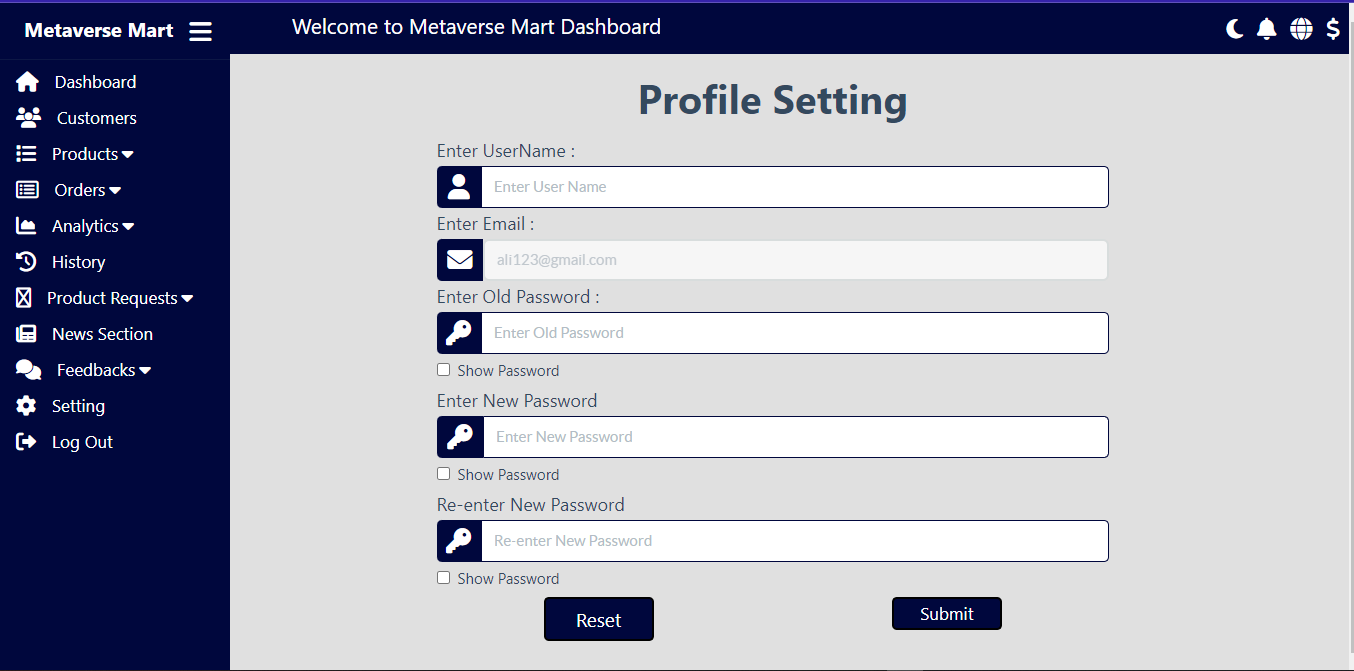
\includegraphics[width=15cm,height=12cm]{Figures/Diagrams/ProfileSetting.PNG}
    \caption{Admin Profile Setting}
    \label{Admin Profile Setting Page}
\end{figure}
\justifying
This image shows the profile setting screen that we have developed for our MetaMart Application for admin of the application. In this screen, there is a form that contains all the fields related to the admin’s profile. This form is fulfilling all validations and valid error messages that would be shown to the user in case of invalid inputs.
\subsubsection{Pending Order}
\begin{figure}[H]
    \centering
    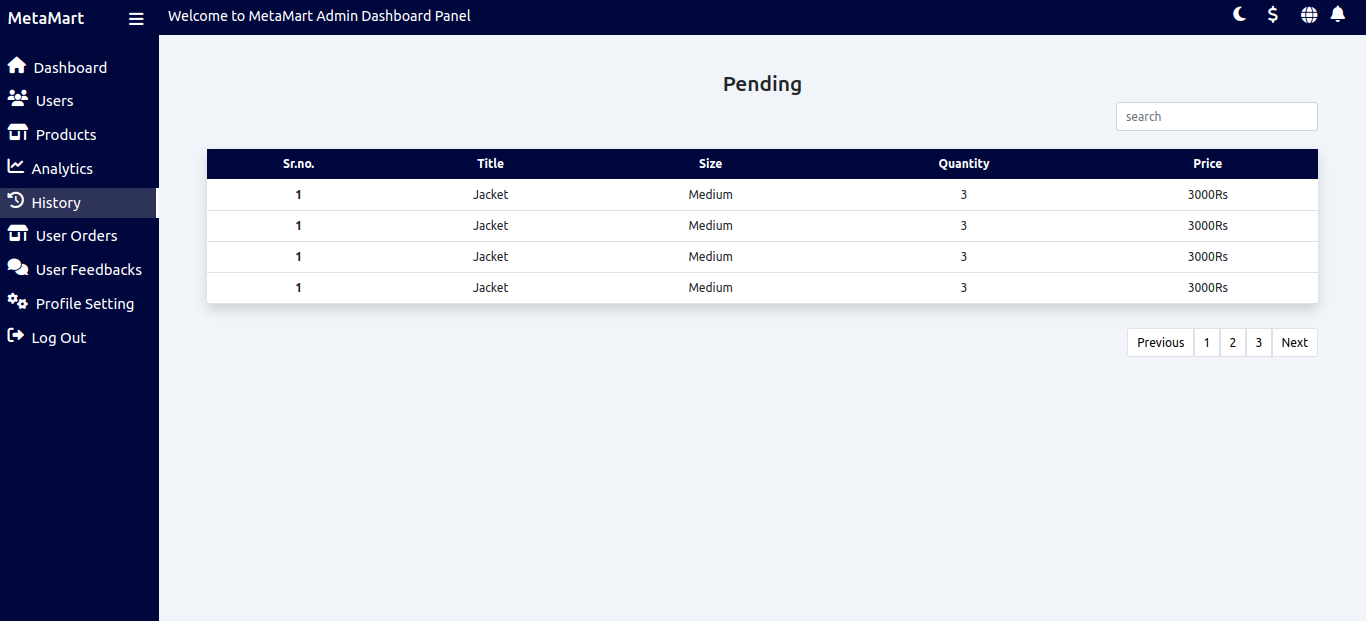
\includegraphics[width=15cm,height=12cm]{Figures/Customer_Section_Images/PendingOrderDetail.png}
    \caption{Admin’s pending orders page}
    \label{Admin’s pending orders page}
\end{figure}
\justifying
This image shows the pending orders screen that we have developed for our MetaMart Application for admin of application. In this screen, there is a table that contains all the orders that are in the queue such that they are not yet received by the customer. Admin can search for an order by order id or simply can explore all orders by next and previous buttons.
\subsection{Customer Section}
\subsubsection{Home Screen}
\begin{figure}[H]
    \centering
    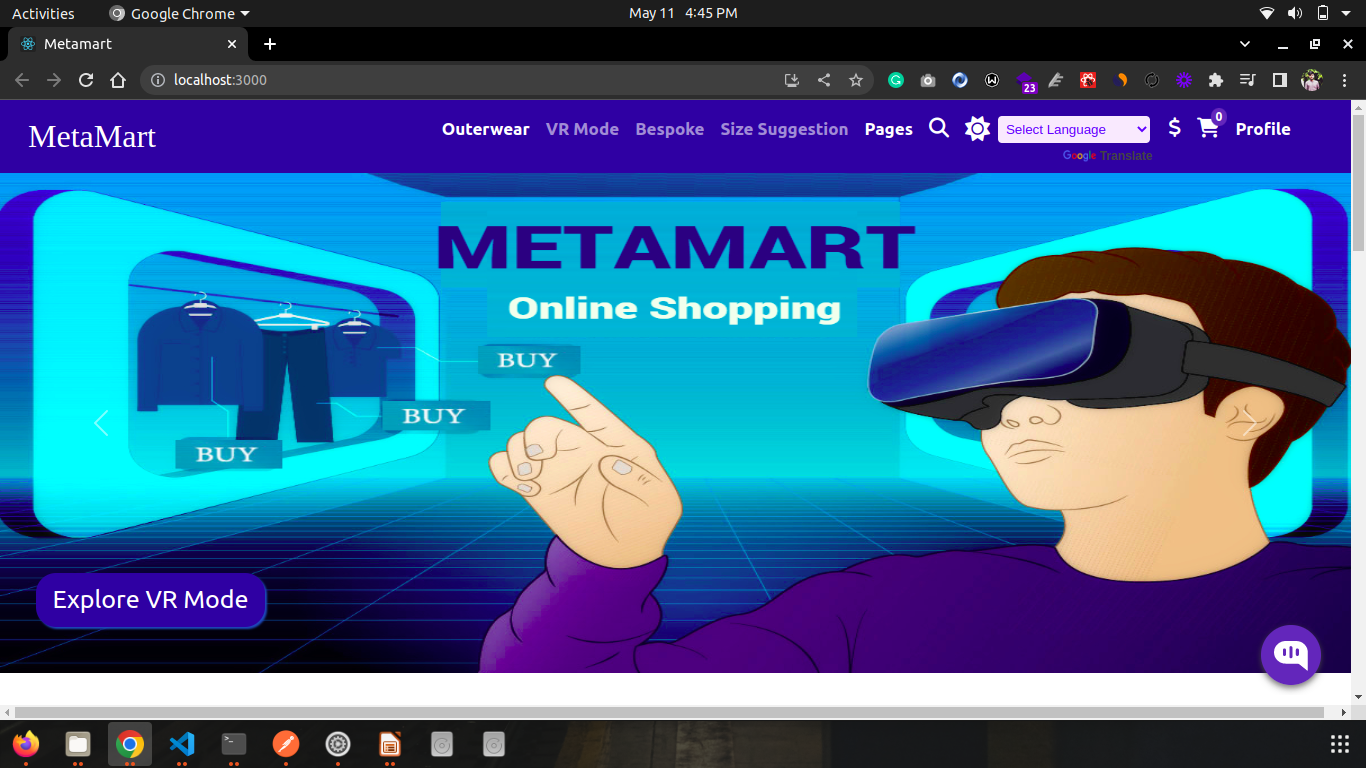
\includegraphics[width=15cm,height=15cm]{Figures/Websites/Customer/customerDashboard.png}
    \caption{Customer’s home page}
    \label{Customer’s home page}
   Home screen for the customer like when the customer will open a virtual reality-based e-commerce web application then this is the main entry point of the website that will be shown to the customer.
\end{figure}
\justifying
This image shows the customer’s home page where the customer would find an option to explore the 3D environment that we have developed for our MetaMart Application. Customers would be able to explore different products just like in the real world.
\subsubsection{Product Section}
\begin{figure}[H]
    \centering
    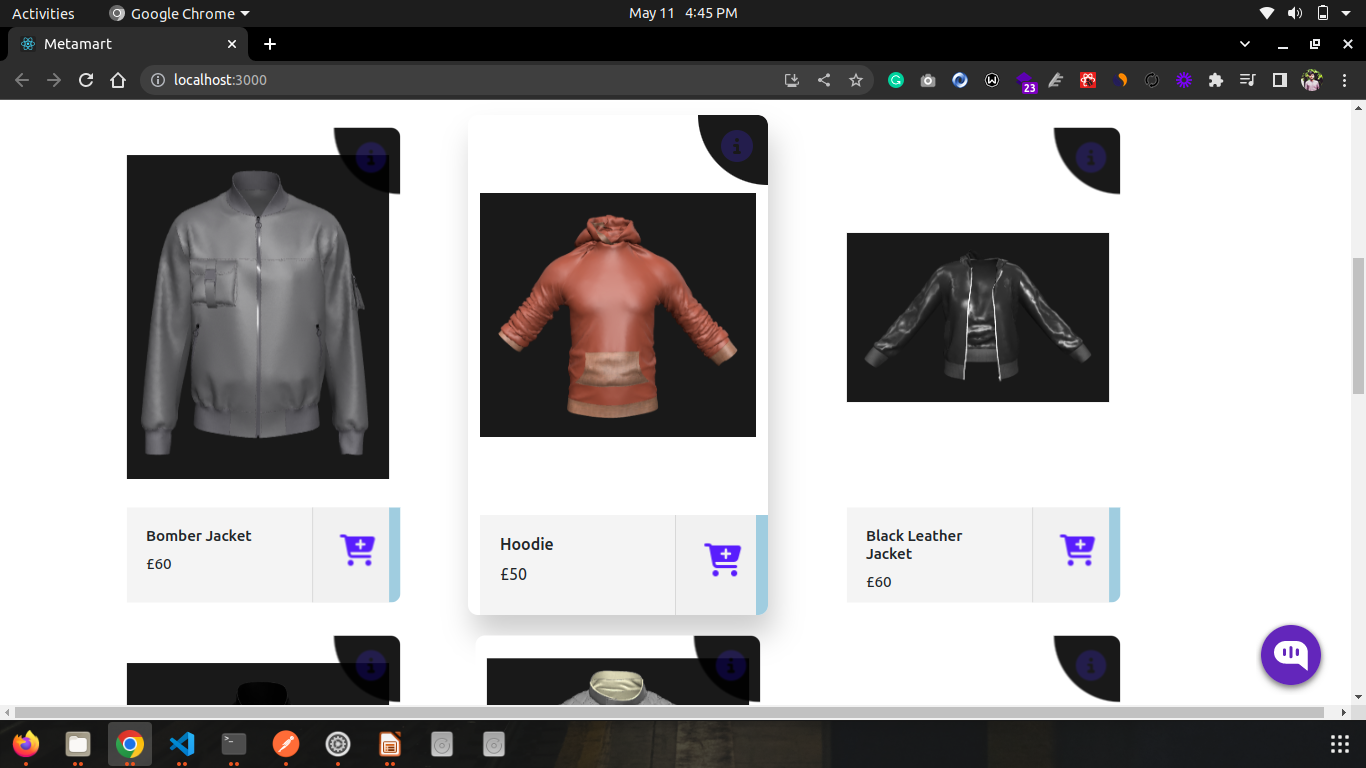
\includegraphics[width=15cm,height=15cm]{Figures/Websites/Customer/CustomerProductList.png}
    \caption{Customer’s products page}
    \label{fig: Product section for customer}
\end{figure}
\justifying
This image shows the customer’s products page where customers would find all products in a general view(2D) just like other e-commerce websites. Here customers can search for a particular product and can see the details of that product by clicking on the details button rendered under every product’s image.
\subsubsection{Signin Section}
\begin{figure}[H]
    \centering
    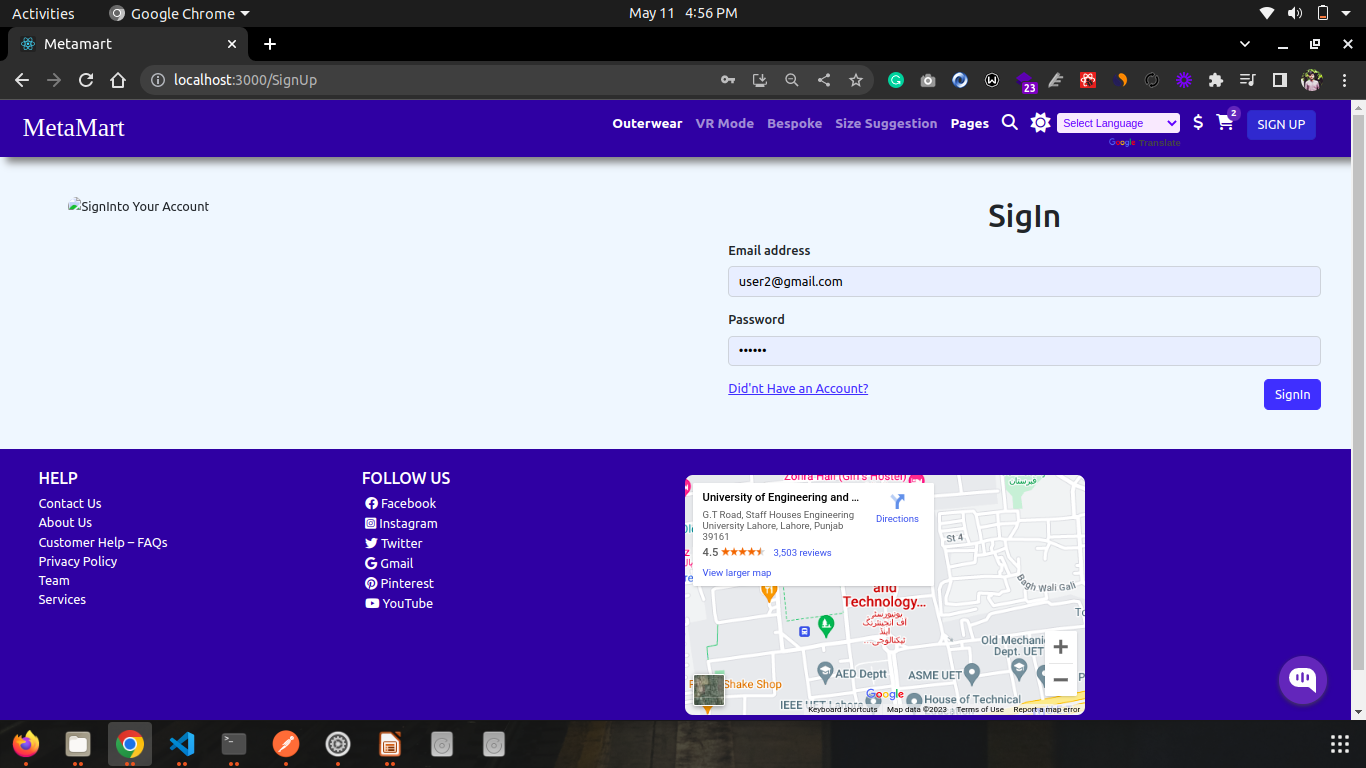
\includegraphics[width=15cm,height=15cm]{Figures/Websites/Customer/CustomerSignin.png}
    \caption{Customer’s products page}
    \label{fig:SignIn Page}
\end{figure}
\justifying

This is the sign-in page where customers can enter their credentials to make a payment for the products they have added to their cart.
\subsubsection{Size suggestion Section}
\begin{figure}[H]
    \centering
    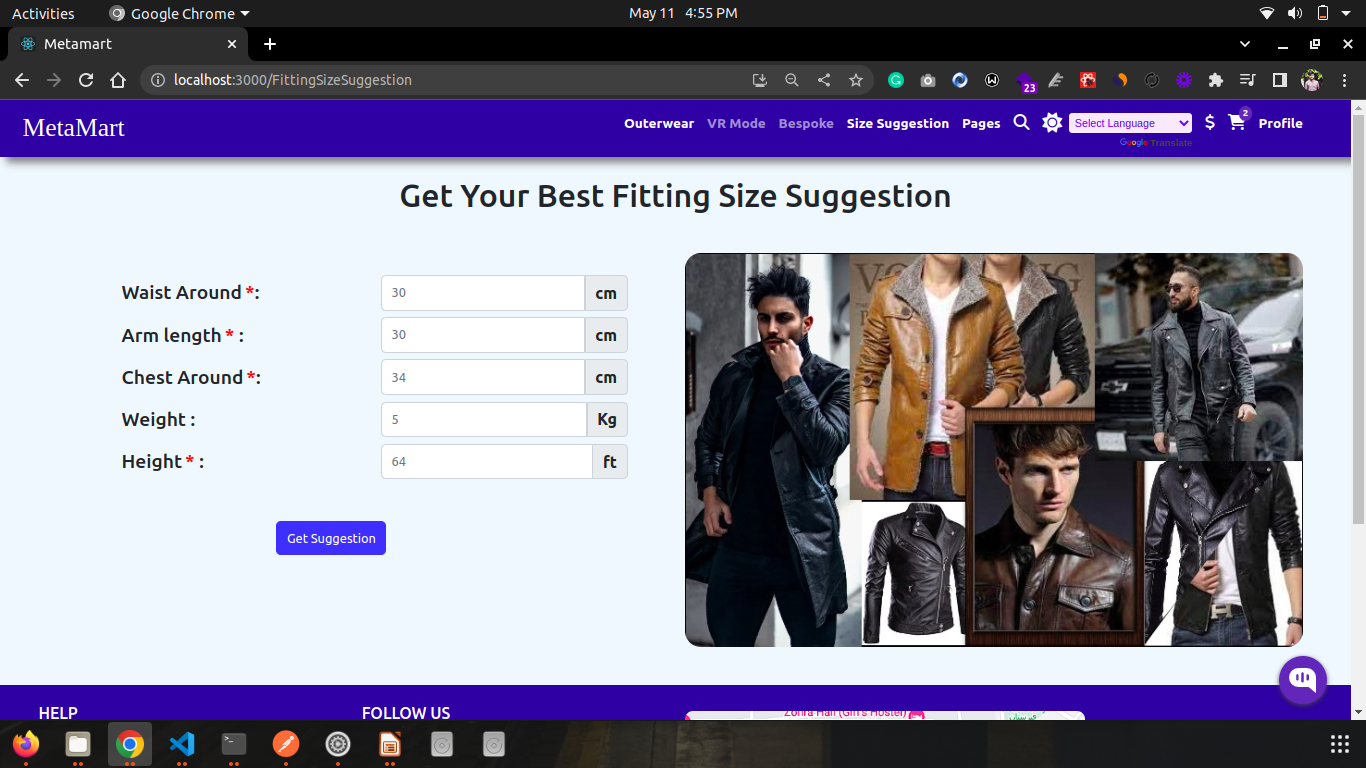
\includegraphics[width=15cm,height=15cm]{Figures/Websites/Customer/CustomerSizeSugestion.png}
    \caption{Customer’s Size suggestion Section}
    \label{fig:Size suggestion Section}
\end{figure}
\justifying

This is the customer size suggestion section. %
% Chapter 5
\newpage
\begingroup%
\makeatletter%
\let\clearpage\relax% Stop LaTeX from going to a new page; and
\vspace*{\fill}%
\vspace*{\dimexpr-50\p@-\baselineskip}% Remove the initial (default) 50pt gap (plus 1 line)
\chapterfont{\centering}
\chapter{Evaluation Criteria}
\vspace*{\fill}%
\endgroup

\newpage
\label{Chapter1}
\lhead{Chapter 5. \emph{Evaluation Criteria}} % Write in your own chapter title to set the page header

\section{TS-1: User Registration Functionality (Customer)}
\subsection{Post-Condition:}
\begin{enumerate}
  \item User is successfully registered and approved by admin.
\end{enumerate}

\begin{table}[H]
    \centering
   \begin{tabular}{ | m{1cm} | m{2.3cm}| m{2cm} | m{2cm} | m{1.7cm} | m{1.3cm} |}  
  \hline  \textbf{Test Case ID} &  \textbf{Description} &  \textbf{Expected Result} &  \textbf{Actual Result} &  \textbf{Executed By} &  \textbf{Status}  \\  \hline
  \textbf{TC-1} & Enter all valid credentials & Successful registration, and “successfully registered message” displayed. & Successful registration, and “successfully registered message” displayed. & Ali & Pass
  \\  \hline
  \textbf{TC-2} & Enter invalid username & Register button should be disable. & Register button disabled. & Ali & Pass
  \\  \hline
  \textbf{TC-3} & Enter invalid email & Register button should be disable. & Register button disabled. & Ali & Pass
  \\  \hline
  \textbf{TC-2} & Enter invalid password & Register button should be disable. & Register button disabled. & Ali & Pass
  \\  \hline
  \textbf{TC-2} & Enter invalid contact info & Register button should be disable. & Register button disabled. & Ali & Pass
  \\  \hline
  
\end{tabular}
    \caption{Test Scenario TS-1 Results}
    \label{tab: Test Scenario TS-1 Results}
\end{table}

\section{TS-2: User Login Functionality}
\subsection{Pre-Condition:}
\begin{enumerate}
  \item User is already registered and approved by admin (except admin).
  \item User is identified and authenticated.
\end{enumerate}
\subsection{Post-Condition:}
\begin{enumerate}
  \item User is successfully logged into the system.
\end{enumerate}

\begin{table}[H]
    \centering
   \begin{tabular}{ | m{1cm} | m{2.3cm}| m{2cm} | m{2cm} | m{1.7cm} | m{1.3cm} |}  
  \hline  \textbf{Test Case ID} &  \textbf{Description} &  \textbf{Expected Result} &  \textbf{Actual Result} &  \textbf{Executed By} &  \textbf{Status}  \\  \hline
  \textbf{TC-1} & Enter all valid credentials & Successful logged in, and “logged in successfully” message should displayed. & Successful logged in, and “logged in successfully” message is displayed. & Ali & Pass
  \\  \hline
  \textbf{TC-2} & Enter invalid username & Login button should be disable. & Login button disabled. & Ali & Pass
  \\  \hline
  \textbf{TC-3} & Enter invalid pass & Login button should be disable. & Login button disabled. & Ali & Pass
  \\  \hline
  
\end{tabular}
    \caption{Test Scenario TS-2 Results}
    \label{tab: Test Scenario TS-2 Results}
\end{table}

\section{TS-3: Manage Product Functionality (Admin)}
\subsection{Pre-Condition:}
\begin{enumerate}
  \item Admin must be logged in to the system.
\end{enumerate}
\subsection{Post-Condition:}
\begin{enumerate}
  \item Admin has access to all functionalities to manage products.
\end{enumerate}

\begin{table}[H]
    \centering
   \begin{tabular}{ | m{1cm} | m{2.3cm}| m{3.3cm} | m{3.3cm} | m{1.7cm} | m{1.3cm} |}  
  \hline  \textbf{Test Case ID} &  \textbf{Description} &  \textbf{Expected Result} &  \textbf{Actual Result} &  \textbf{Executed By} &  \textbf{Status}  \\  \hline
  \textbf{TC-1} & Adding new product with valid details & Successful add new product, and “product added successfully” message should display. & Successful add new product, and “product added successfully” message displayed. & Ehtesham & Pass
  \\  \hline
  \textbf{TC-2} & Adding new product with any invalid detail & Add button should be disabled. & Add button disabled. & Ehtesham & Pass
  \\  \hline
  \textbf{TC-3} & Entering valid ID to Delete/Remove any unwanted product & Deleted successfully, a “product removed successfully” message should be displayed, and redirects admin to the dashboard main section. & Deleted successfully, a “product removed successfully” message should be displayed, and redirects admin to the dashboard main section. & Ehtesham & Pass
  \\  \hline
  \textbf{TC-4} & Entering invalid ID to Delete/Remove any unwanted product & “Incorrect product ID”/ “Product id does not exist” error message should display. & “Incorrect product ID”/ “Product id does not exist” error message is displayed. & Ehtesham & Pass
  \\  \hline
  \textbf{TC-5} & Entering valid ID to search product & Product should display successfully & Product displayed successfully. & Ehtesham & Pass
  \\  \hline
  \textbf{TC-6} & Entering invalid ID to search product & “Incorrect product ID”/ “Product id does not exist” error message should display. & “Incorrect product ID”/ “Product id does not exist” error message is displayed. & Ehtesham & Pass
  \\  \hline
  \textbf{TC-7} & Update any product with valid details & Successfully update product, and “product updated successfully” message should display. & Successfully update product, and “product updated successfully” message is displayed. & Ehtesham & Pass
  \\  \hline
  \textbf{TC-8} & Update any product with any invalid details & Update button should remain disable. & Update button remain disable. & Ehtesham & Pass
  \\  \hline
  
\end{tabular}
    \caption{Test Scenario TS-3 Results}
    \label{tab: Test Scenario TS-3 Results}
\end{table}

\section{TS-4: Manage Customize orders Functionality (Admin)}
\subsection{Pre-Condition:}
\begin{enumerate}
  \item Admin must be logged in to the system.
\end{enumerate}
\subsection{Post-Condition:}
\begin{enumerate}
  \item Admin has access to manage customized orders of customers.
\end{enumerate}

\begin{table}[H]
    \centering
   \begin{tabular}{ | m{1cm} | m{2.5cm}| m{2.7cm} | m{2.7cm} | m{1.7cm} | m{1.3cm} |}  
  \hline  \textbf{Test Case ID} &  \textbf{Description} &  \textbf{Expected Result} &  \textbf{Actual Result} &  \textbf{Executed By} &  \textbf{Status}  \\  \hline
  \textbf{TC-1} & Checking customers customized orders’ requests. & All customize orders’ request should displayed. & All customize orders’ request are displayed. & Ali & Pass
  \\  \hline
  
\end{tabular}
    \caption{Test Scenario TS-4 Results}
    \label{tab: Test Scenario TS-4 Results}
\end{table}


\section{TS-5: Manage Profile Functionality}
\subsection{Pre-Condition:}
\begin{enumerate}
  \item Customer must be registered.
  \item Customer must be authenticated and identified.
  \item Customer must be logged in to the system.
\end{enumerate}
\subsection{Post-Condition:}
\begin{enumerate}
  \item Customer Profile will get updated.
\end{enumerate}

\begin{table}[H]
    \centering
   \begin{tabular}{ | m{1cm} | m{2.3cm}| m{3cm} | m{3cm} | m{1.7cm} | m{1.3cm} |}  
  \hline  \textbf{Test Case ID} &  \textbf{Description} &  \textbf{Expected Result} &  \textbf{Actual Result} &  \textbf{Executed By} &  \textbf{Status}  \\  \hline
  \textbf{TC-1} & Update profile with valid details & Successfully update profile, and “profile updated successfully” message should display. & Successfully update profile, and “profile updated successfully” message is display. & Abdullah & Pass
  \\  \hline
  \textbf{TC-2} & Update profile with invalid details & Update button should remain disable. & Update button remain disable. & Abdullah & Pass
  \\  \hline
  
\end{tabular}
    \caption{Test Scenario TS-5 Results}
    \label{tab: Test Scenario TS-5 Results}
\end{table}

\section{TS-6: Virtual Tour Functionality (customer)}
\subsection{Pre-Condition:}
\begin{enumerate}
  \item Customer must be registered.
  \item Customer must be authenticated and identified.
  \item Customer must be logged in to the system.
  \item Customer must have entered in virtual tour mode.
\end{enumerate}
\subsection{Post-Condition:}
\begin{enumerate}
  \item Customer can experience all real time shopping functionalities.
\end{enumerate}

\begin{table}[H]
    \centering
   \begin{tabular}{ | m{1cm} | m{2.3cm}| m{3cm} | m{3cm} | m{1.7cm} | m{1.3cm} |}  
  \hline  \textbf{Test Case ID} &  \textbf{Description} &  \textbf{Expected Result} &  \textbf{Actual Result} &  \textbf{Executed By} &  \textbf{Status}  \\  \hline
  \textbf{TC-1} & Experiencing virtual tour without any issue & Virtual view of mall and functionalities should be visible to the user. & Virtual view of mall and functionalities is visible to the user. & Maham & Pass
  \\  \hline
  \textbf{TC-2} & Experiencing virtual tour with any issue & Virtual view of mall should not be visible to the user, and appropriate error message should be displayed. & Virtual view of mall is not visible to the user, and appropriate error message is displayed. & Maham & Pass
  \\  \hline
  \textbf{TC-3} & Visit virtual store & Customer’s avatar should roam around the virtual store to take a tour. & Customer’s avatar can take the tour of virtual store. & Maham & Pass
  \\  \hline
  \textbf{TC-4} & Showing Jackets details & Jackets’ details should be popped up on triggering with the avatar. & Jackets’ details are popping on a panel when avatar is triggered with the any jacket. & Maham & Pass
  \\  \hline
  \textbf{TC-5} & Jackets Size Options & There should be four size displaying options available for jackets for 4 standard body sizes. & Options for 4 standard sizes jackets are available in the store with details. & Maham & Pass
  \\  \hline
  \textbf{TC-6} & Mannequin Avatar dynamic Size  & The avatar size should be change during run-time according to the customers’ selected jacket size. & The avatar size can be change during run-time according to the selected jacket size. & Maham & Pass
  \\  \hline
  \textbf{TC-7} & Add to cart  & Customers should add the choosed jackets to cart from virtual store also. & Customer can also add to cart the choosed items from the virtual store. & Maham & Pass
  \\  \hline
  
\end{tabular}
    \caption{Test Scenario TS-6 Results}
    \label{tab: Test Scenario TS-6 Results}
\end{table}

\section{TS-7: Manage cart Functionality(customer)}
\subsection{Pre-Condition:}
\begin{enumerate}
  \item Customer must be registered.
  \item Customer must be authenticated and identified.
  \item Customer must be logged in to the system.
\end{enumerate}
\subsection{Post-Condition:}
\begin{enumerate}
  \item Customer can manage personal cart section.
\end{enumerate}

\begin{table}[H]
    \centering
   \begin{tabular}{ | m{1cm} | m{2.5cm}| m{2.7cm} | m{2.7cm} | m{1.7cm} | m{1.3cm} |}  
  \hline  \textbf{Test Case ID} &  \textbf{Description} &  \textbf{Expected Result} &  \textbf{Actual Result} &  \textbf{Executed By} &  \textbf{Status}  \\  \hline
  \textbf{TC-1} & Adding items to cart & Selected item should be added in the cart list and should stay even after logged out until gets removed or delivered. & Selected item gets added in the cart list and remain in list even after logged out until gets removed or delivered. & Abdullah & Pass
  \\  \hline
  \textbf{TC-2} & Updating cart items & Items added in the cart should get updated. & Cart items gets updated. & Abdullah & Pass
  \\  \hline
  
\end{tabular}
    \caption{Test Scenario TS-7 Results}
    \label{tab: Test Scenario TS-7 Results}
\end{table}

\section{TS-8: Customize Order Request(customer)}
\subsection{Pre-Condition:}
\begin{enumerate}
  \item Customer must be registered.
  \item Customer must be authenticated and identified.
  \item Customer must be logged in to the system.
\end{enumerate}
\subsection{Post-Condition:}
\begin{enumerate}
  \item Customer can request for any customized order.
\end{enumerate}

\begin{table}[H]
    \centering
   \begin{tabular}{ | m{1cm} | m{2.5cm}| m{2.7cm} | m{2.7cm} | m{1.7cm} | m{1.3cm} |}  
  \hline  \textbf{Test Case ID} &  \textbf{Description} &  \textbf{Expected Result} &  \textbf{Actual Result} &  \textbf{Executed By} &  \textbf{Status}  \\  \hline
  \textbf{TC-1} & Adding customized order details & Customized order details should get added into the request section and notification should be sent to the admin. & Customized order details get add into the request section and notification has sent to the admin. & Maham & Pass
  \\  \hline
  \textbf{TC-2} & Checking response status from store service about customized order request. & The request status should be displayed in the request status. & The request status displays in the request status. & Maham & Pass
  \\  \hline
  
\end{tabular}
    \caption{Test Scenario TS-8 Results}
    \label{tab: Test Scenario TS-8 Results}
\end{table}

\section{TS-9: Payment Section Functionality (customer)}
\subsection{Pre-Condition:}
\begin{enumerate}
  \item Customer must be registered.
  \item Customer must be authenticated and identified.
  \item Customer must be logged in to the system.
\end{enumerate}
\subsection{Post-Condition:}
\begin{enumerate}
  \item Customer can request for any customized order.
\end{enumerate}

\begin{table}[H]
    \centering
   \begin{tabular}{ | m{1cm} | m{2.5cm}| m{2.7cm} | m{2.7cm} | m{1.7cm} | m{1.3cm} |}  
  \hline  \textbf{Test Case ID} &  \textbf{Description} &  \textbf{Expected Result} &  \textbf{Actual Result} &  \textbf{Executed By} &  \textbf{Status}  \\  \hline
  \textbf{TC-1} & Entering all valid credentials for payment & Payment gets done and “payment done successfully” message should display on screen. & Payment gets done and “payment done successfully” message displays on screen. & Ali & Pass
  \\  \hline
  \textbf{TC-2} & Entering any invalid credentials for payment & Payment proceeds button should remain disable. & Payment proceeds button remain disable. & Ali & Pass
  \\  \hline
  
\end{tabular}
    \caption{Test Scenario TS-9 Results}
    \label{tab: Test Scenario TS-9 Results}
\end{table}

\section{TS-10: Product Rating Functionality (customer)}
\subsection{Pre-Condition:}
\begin{enumerate}
  \item Customer must be registered.
  \item Customer must be authenticated and identified.
  \item Customer must be logged in to the system.
  \item Customer must has already received that specific product.
\end{enumerate}
\subsection{Post-Condition:}
\begin{enumerate}
  \item Customer will be able to give rating about any received product. 
\end{enumerate}

\begin{table}[H]
    \centering
   \begin{tabular}{ | m{1cm} | m{2.5cm}| m{2.7cm} | m{2.7cm} | m{1.7cm} | m{1.3cm} |}  
  \hline  \textbf{Test Case ID} &  \textbf{Description} &  \textbf{Expected Result} &  \textbf{Actual Result} &  \textbf{Executed By} &  \textbf{Status}  \\  \hline
  \textbf{TC-1} & Rating received products & Rating should be added and a “Thank you!” message should be displayed. & Rating is added and a “Thank you!” message is displayed. & Ehtesham & Failed
  \\  \hline
  
\end{tabular}
    \caption{Test Scenario TS-10 Results}
    \label{tab: Test Scenario TS-10 Results}
\end{table}

\justifying
 %
% Chapter 5
\newpage
\begingroup%
\makeatletter%
\let\clearpage\relax% Stop LaTeX from going to a new page; and
\vspace*{\fill}%
\vspace*{\dimexpr-50\p@-\baselineskip}% Remove the initial (default) 50pt gap (plus 1 line)
\chapterfont{\centering}
\chapter{Future Work}
\vspace*{\fill}%
\endgroup

\newpage
\label{Chapter6}
\lhead{Chapter 6. \emph{Future Work}} % Write in your own chapter title to set the page header
We aimed to develop a virtual reality-based E-Commerce web application called MetaMart, which provides customers with a realistic shopping experience in the Metaverse. This project involves developing a basic E-Commerce website with all necessary features, integrating a 3D tour and VR mode created in Unity 3D into the website, placing 3D clothing on an avatar with custom dimensions focused on providing customers with a personalized shopping experience.
The use of virtual reality technology in your application allows you to provide your customers with an immersive and realistic shopping experience. This is a vast improvement over traditional online shopping experiences based on 2D images and descriptions. By implementing the metaverse concept, applications can get a glimpse into the future of shopping in virtual worlds. 
\section{Future Work}
The current project has achieved the desired goals. However, there is still room for improvement and further development in the future. The next section outlines future work that can be done to improve the MetaMart application.

\textbf{1. Product extensions:}

The current MetaMart application focuses on providing an apparel and outerwear shopping experience. In the future, the application can be extended to other products such as accessories, shoes and electronics. This allows you to have more product diversity for your customers and attract a wider audience.

\textbf{2. Artificial intelligence integration:}

MetaMart applications can be further enhanced by integrating artificial intelligence (AI) technology to provide personalized recommendations based on the customer's shopping history, preferences, and behavior. AI algorithms can analyze customer data and suggest products that match customer interests to improve customer satisfaction and sales.

\textbf{3. Enhanced virtual reality experience:}

VR experiences can be enhanced by incorporating haptic feedback and better graphics to create a more immersive and realistic shopping experience. This can be achieved through the use of advanced VR technologies such as haptic gloves and full-body tracking systems.

\textbf{4. Integration with social media:}

MetaMart's integration with social media platforms allows customers to share their shopping experience with friends and family, creating a sense of community around the application. Additionally, you can use social media integration to promote your products and increase brand awareness.

\textbf{5. Integration with blockchain technology:}

Blockchain technology can be integrated into his MetaMart application for greater security and transparency. This can be achieved by implementing a decentralized system that tracks transaction and product authenticity, ensuring that customers receive genuine products. 6. Multilingual support:

MetaMart can be extended to support multiple languages, making it accessible to more users. This allows customers in different regions to access the application in their native language, improving user experience and customer satisfaction.

\textbf{7. Performance optimization:}

MetaMart application performance can be further optimized by reducing load times, reducing latency, and minimizing crashes and errors. This improves the overall user experience and ensures your application runs smoothly and efficiently.

In summary, the MetaMart project has demonstrated the potential of virtual reality technology in the e-commerce industry. Future work outlined above may help further develop and improve the application and provide customers with a more satisfying and immersive shopping experience in the Metaverse.  %
%\newpage

% Chapter 3
 % Write in your own chapter title
\begingroup%
\makeatletter%
\let\clearpage\relax% Stop LaTeX from going to a new page; and
\vspace*{\fill}%
\vspace*{\dimexpr-50\p@-\baselineskip}% Remove the initial (default) 50pt gap (plus 1 line)
\chapterfont{\centering}
\chapter{Proposed Methodology}
\vspace*{\fill}%
\endgroup

\newpage
\label{Chapter3}
\lhead{Chapter 3. \emph{Proposed Methodology}} % Write in your own chapter title to set the page header

\section{General Flow}
The web application we developed offers a wide range of key functionalities and is
easy to use. Our application is designed primarily for administrators and online
users having VR headsets and those who don't have VR headsets as well. The admin can add new products, delete products, update deleted products, view reports/statistics, customer lists, and pending and completed orders. The admin can also update his account setting if necessary. While on the other hand, the customer can visit the website with and without a VR headset as well. Those customers having Oculus VR headsets can experience virtual reality-based MetaMart while customers without VR headsets can do a 3D tour of the MetaMart. The customer can also request some products if not available in our store. Following are some of the diagrams that will help you to understand the sequence flow of our application.
\section{Software development methodology}
We are using Agile methodology.
\subsection{Road map}
Our main goal is to revolutionize the idea of E-Commerce business to facilitate the customer with an immersive and modern virtual platform to bridge the gap between the real and virtual shopping experience. So, to accomplish this goal we came after with the following steps:
\begin{enumerate}
    \item 	Exploring related existing past work (if any), wade through the research papers, articles, and generals. Endeavor to perceive the gaps of prior related works.
    \item Defining a working methodology, which software development approach we are going to manipulate throughout the whole development process.
    \item Specifying the functional and non-functional requirements for the targeted vision.
    \item Conducting feasibility study to contemplate all the aspects of the purposed application model to assemble an estimation is respect to accomplishment extent.
    \item Creating a general flow diagram to accentuate the workflow of the proposed application. Then, design several diagrams including a general diagram, data flow diagram (level0 and level1), use case diagram (general and detailed), flow chart, class diagram, entity-relationship diagram, and sequence diagram to clarify every aspect in a detailed way. 
     \item Note down all the use cases for the MetaMart application.
    \item Afterwards, select the tools and technology going to operate throughout the entire proposal implementation.
    \item Designing the wireframes for web configuration of the virtual environment.
    \item Designing a virtual 3D virtual store in meta verse , 3D clothes, 3D avatars.
    \item Designing the prototype to delineate an explicit scheme of how the proposed application is going to operate.
    \item Finally, developing the MetaMart website and integrating it with the 3D virtual environment made with Unity framework to make the complete system in a fine useable form.
    \item Testing the entire developed system and performing the test case scenarios and evaluating the project according to the test case scenarios.
\end{enumerate}
Feasibility Study:
i)	Economic feasibility:
1.  Web development: almost cost none.
2.  API: some APIs require purchase, so it will account for cost.
3.  Hardware: Our project requires some hardware devices (VR Headsets) which add to the cost of our project. So, to fulfill our economical requirements, we have applied for funding assistance on Ignite FYP funding assistance through the NGIRI portal.

\subsection{Technical feasibility}
The 3D virtual tour and 3D virtual store experience with a VR headset are achievable. With the help of currently available tools to us, it's difficult to make avatars with customized customer input sizes. Regular MetaMart with advanced features like advanced searching filtering, easy navigation, and social media sharing button integration can be done.

\subsection{Operational feasibility}
we will analyze whether our project will work accordingly in the same way as decided. we will also check whether all the features are implemented in the project. So, all the requirements will be fulfilled. we will also keep in the view that our website will be easy to use for customers and should be understandable.

\subsection{	Schedule feasibility}
As for the development process, we will follow the agile methodology in which we will design weekly sprints and in each scheduled meeting, we will improve our system timely. So in his way, the proper schedule will be followed and our product will be completed by the end within the due timeline.

\section{General Proposed Model}
\begin{figure}[H]
    \centering
    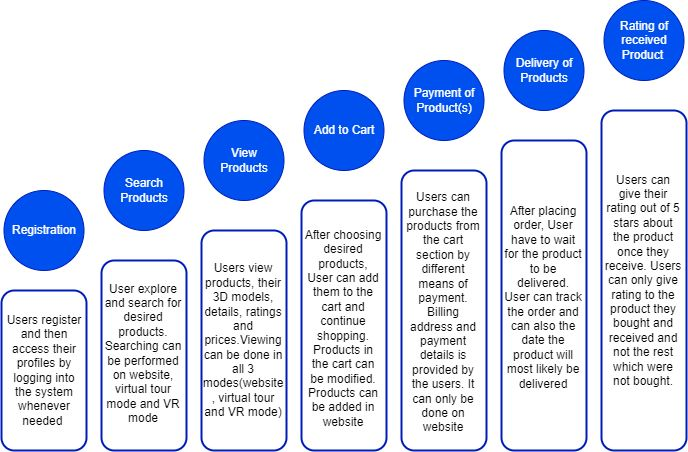
\includegraphics[width=15cm,height=10cm]{Figures/Diagrams/GeneralProposedModel.jpeg}
    \caption{General Proposed Model
     of Virtual Reality-based MetaMart Web Application
     }
    \label{fig: General Proposed Model}
   General Proposed Model
     of Virtual Reality-based MetaMart Web Applications.
\end{figure}
\section{Data Flow Diagram}
Following are the data flow diagrams of the Virtual reality-based MetaMart web application:
\subsection{Data Flow Diagram Level0}
\begin{figure}[H]
    \centering
    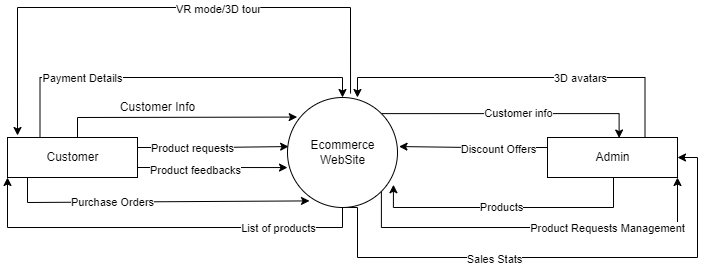
\includegraphics[width=15cm,height=8cm]{Diagrams/dfdlevel0.png}
    \caption{System’s Data Flow Diagram (Level-0)}
    \label{fig: System’s Data Flow Diagram (Level-0)}
\end{figure}
 \justifying
    This diagram illustrates the flow of data between 3 major components of the system which are the customer, admin, and web application. This figure describes which data would be flowing from which source to which destination. As some data like customer information would be flowing from customers towards the application. Similarly, product data would be entered by the admin so this data would be flowing from the admin toward the application. 
\subsection{Data Flow Diagram Level1}
\begin{figure}[H]
    \centering
    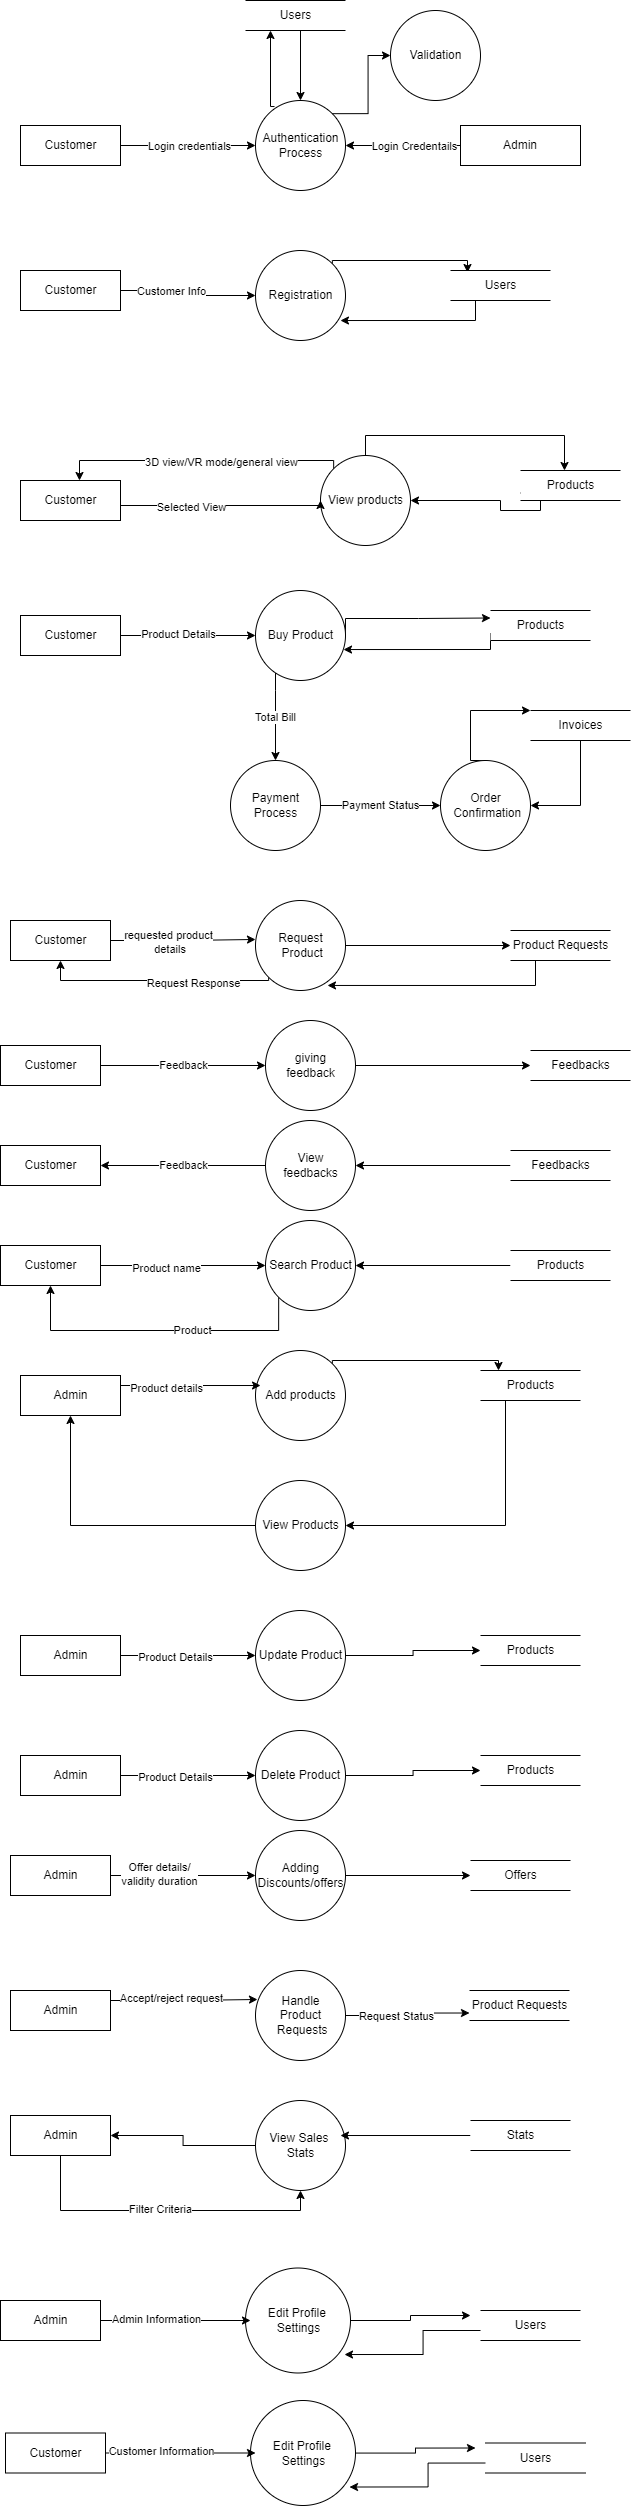
\includegraphics[width=12cm,height=25cm]{Diagrams/dfdlevel1.png}
    \caption{System’s Data Flow Diagram (Level-1)}
    \label{fig: System’s Data Flow Diagram (Level-1)}
\end{figure}
 \justifying
    This diagram illustrates the flow of data between the system’s components by reducing the abstraction level. In this diagram application component in the level-0 diagram is divided into some important modules like giving feedback, making an order, making payment, updating customers’ information, handling request, and many others shown in the diagram. All these modules represent the direction of data, the data which a module consumes or sends to any other dependent module or database.
\section{Use Case Diagram}
In the below section, you will see the General use case diagram and detailed use case diagram of the website as well that describe the high-level functions and scope of a system. 
\subsection{General Diagram}
\begin{figure}[H]
    \centering
    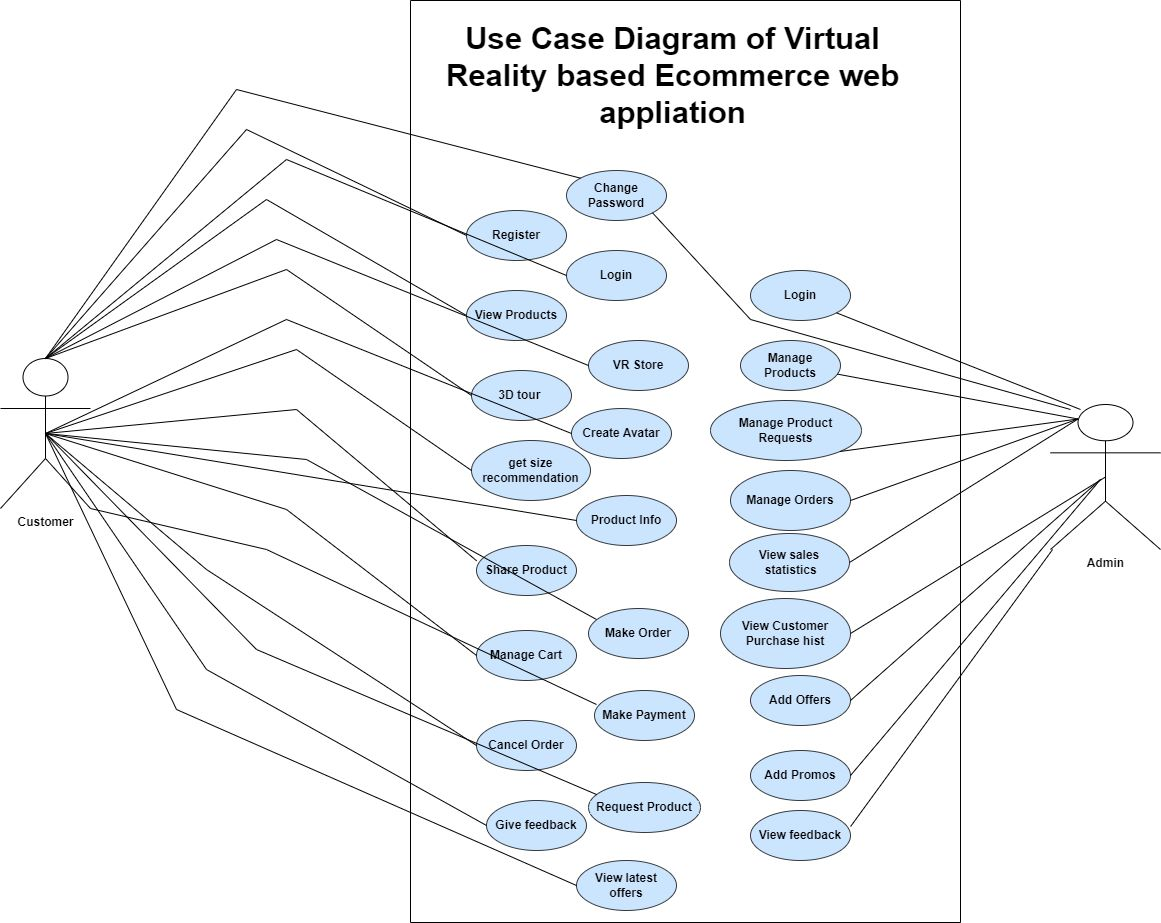
\includegraphics[width=15cm,height=15cm]{Diagrams/GeneralUseCaseDiagram.jpeg}
    \caption{General class Diagram}
    \label{fig: General Use case diagram}
   \justifying
   This diagram represents the general use cases with higher abstraction levels. All the use cases of entities(customer and admin represented by avatars in the diagram) are listed by associating them with the respective entity’s avatar. For example, login is a use case so this use case is associated with the admin’s as well as the customer’s avatar.
\end{figure}
\subsection{Detailed Use case diagram}
\begin{figure}[H]
    \centering
    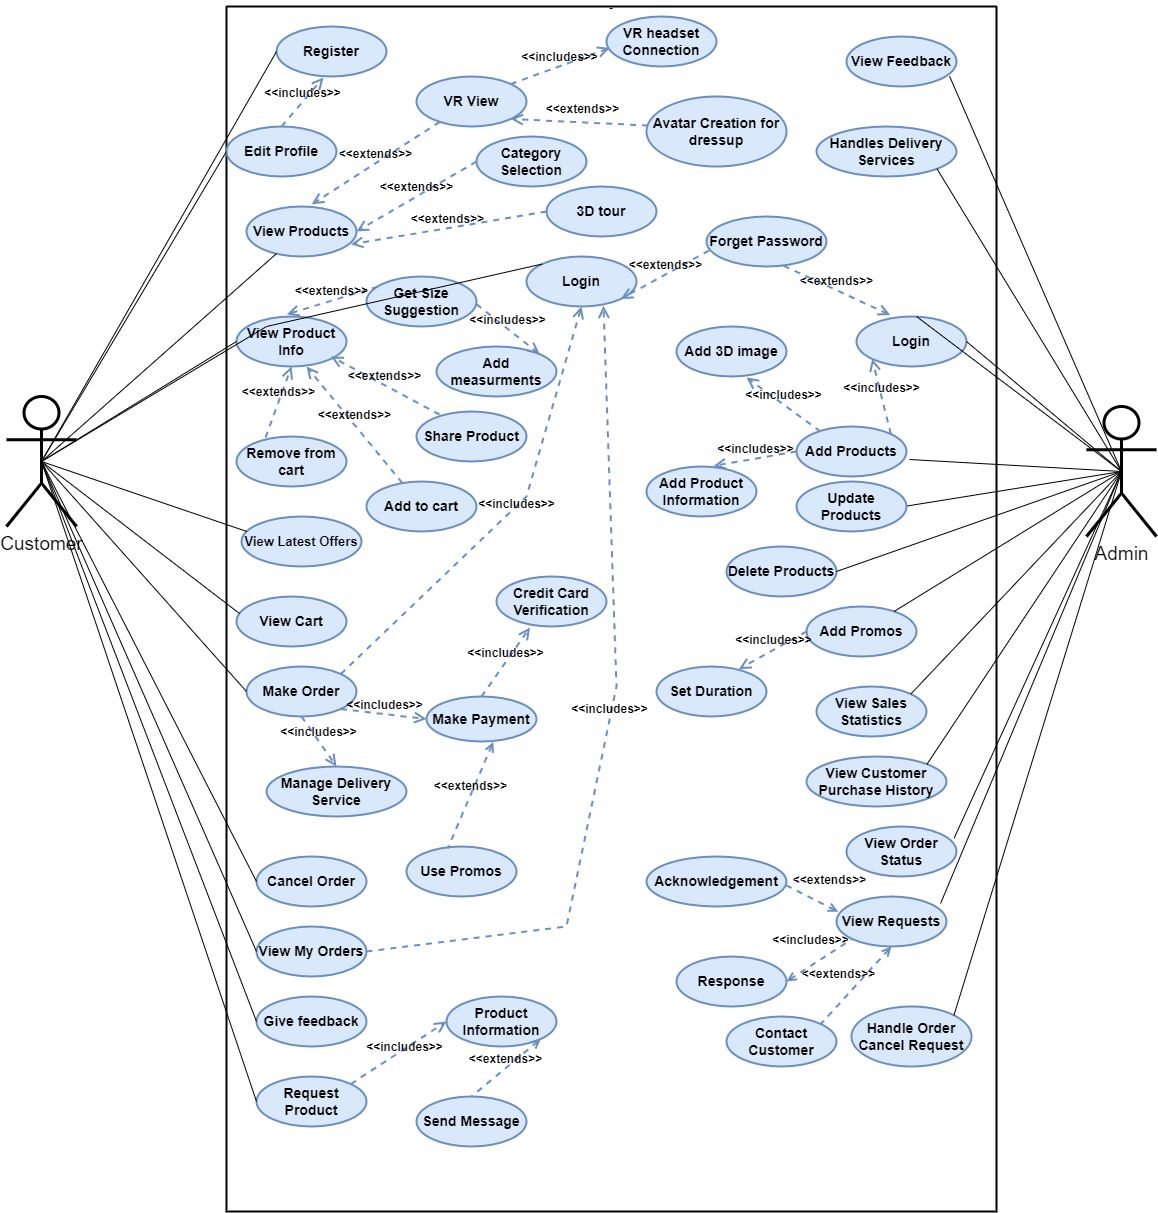
\includegraphics[width=15cm,height=15cm]{Diagrams/DetailUsedCaseDiagram.jpeg}
    \caption{Detailed Use case diagram}
    \label{fig: Detailed Use case diagram}
\end{figure}
\justifying
This diagram represents the detailed use cases. All the use cases of entities are listed along with the relationship(extend/includes) between use cases. For example, login is a use case but another use case which is forgetting the password extends this use case. Similarly, making an order includes making a payment because to complete the first use case (make order),  it is necessary to fulfill included use case which makes payment.
\section{Use Cases}
Following are the actors in our virtual Reality-based MetaMart web application:
\begin{enumerate}
    \item Admin
    \item Customer
\end{enumerate}
\subsection{Use Case of Admin Section}
\subsubsection{Use Case UC-1: Admin Login }
\textbf{Description:}\\
The following use case is about successful administrator login after providing valid login details.
\\
\textbf{Pre-Conditions:}
\begin{enumerate}
    \item Admin should have already been registered.
    \item  All required information about the admin should be available in the database.
    \item Databases should be available.
\end{enumerate}
\textbf{Normal Flow:}\\
\begin{enumerate}
\item The administrator enters valid login details.
\item Administrator clicks on the login button.
\item System confirms and validates the data. 
\item Admin successfully logins the account.
\end{enumerate}
\textbf{Post-Conditions: }
\begin{enumerate}
\item	Admin successfully logins the account. 
\end{enumerate}
\textbf{Authority:}
Administrator
\subsubsection{Use Case UC-2: Add Products }
\textbf{Description:}\\
The following use case is about managing and adding products to the existing system.
\\
\textbf{Pre-Conditions:}
\begin{enumerate}
    \item  All required information about the admin should be available.
    \item Databases should be available.
\end{enumerate}
\textbf{Normal Flow:}\\
\begin{enumerate}
\item Administrator has the option to add a new product.
\item System asks for necessary information regarding the product.
\item Administrator provides all the required information to complete the operation.
\item System after confirmation adds the new product.
\end{enumerate}
\textbf{Post-Conditions: }
\begin{enumerate}
\item	A new user account is successfully created.
\end{enumerate}
\textbf{Authority:}
Administrator
\subsubsection{ Use Case UC-3: Edit Product Details}
\textbf{Description:}\\
The following use case is about managing editing/modifying Product details in the existing system.
\\
\textbf{Pre-Conditions:}
\begin{enumerate}
    \item  All required information about the admin should be available.
    \item Databases should be available.
\end{enumerate}
\textbf{Normal Flow:}\\
\begin{enumerate}
\item Administrator options to edit the product details(title, description, images, etc).
\item Administrator changes the desired details of the product options to complete the operation.
\item System after confirmation updates the details of the product in the database and the website as well.
\end{enumerate}
\textbf{Post-Conditions: }
\begin{enumerate}
\item	The product will be live on the website with updated new details successfully.
\end{enumerate}
\textbf{Authority:}
Administrator
\subsubsection{ Use Case UC-4: Delete Products}
\textbf{Description:}\\
The following use case is about managing to delete products in the existing system.\\
\textbf{Pre-Conditions:}
\begin{enumerate}
    \item  All required information about the admin should be available.
    \item Databases should be available.
\end{enumerate}
\textbf{Normal Flow:}\\
\begin{enumerate}
\item Administrator options to delete a product.
\item The administrator will click on the delete product option and then the system will ask for confirmation before deleting the product from the database.
\item System after confirmation deletes the product from the database.
\end{enumerate}
\textbf{Post-Conditions: }
\begin{enumerate}
\item	The desired product is successfully deleted from the database.
\end{enumerate}
\textbf{Authority:}
Administrator
\subsubsection{ Use Case UC-5: View Products}
\textbf{Description:}\\
The following use case is about viewing products in the existing system.
\\
\textbf{Pre-Conditions:}
\begin{enumerate}
    \item Admin must be logged in to the system.
    \item  All required information about the admin should be available.
    \item Database should be available.
\end{enumerate}
\textbf{Normal Flow:}\\
\begin{enumerate}
\item Administrator options to view a new product.
\item Administrator can see all the products.
\end{enumerate}
\textbf{Post-Conditions: }
\begin{enumerate}
\item	All the products will be displayed to the administrator.
\end{enumerate}
\textbf{Authority:}
Administrator
\subsubsection{ Use Case UC-6: Search Products}
\textbf{Description:}\\
The following use case is about searching for products in the existing system.\\
\textbf{Pre-Conditions:}
\begin{enumerate}
    \item  All required information about the admin should be available.
    \item Database should be available.
\end{enumerate}
\textbf{Normal Flow:}\\
\begin{enumerate}
\item Administrator options to search a product.
\item System asks for necessary information.
\item Administrator provides the name of the product or sets the price range.
\item System after taking administrator shows the results.
\end{enumerate}
\textbf{Post-Conditions: }
\begin{enumerate}
\item	The desired products will be displayed to the admin
\end{enumerate}
\textbf{Authority:}
Administrator
\subsubsection{ Use Case UC-7: View Orders and purchase history of Products}
\textbf{Description:}\\
The following use case is about viewing orders and the purchase history of products in the existing system.
\\
\textbf{Pre-Conditions:}
\begin{enumerate}
    \item  All required information about the admin should be available.
    \item Database should be available.
\end{enumerate}
\textbf{Normal Flow:}\\
\begin{enumerate}
\item Administrator options to about viewing orders and purchase history of products in the existing system.
\item The system will display the orders and purchase history.
\end{enumerate}
\textbf{Post-Conditions: }
\begin{enumerate}
\item	The orders and purchase history of products will be displayed to the admin\end{enumerate}
\textbf{Authority:}
Administrator

\subsubsection{ Use Case UC-8: View Customer Details except for Personal information (account password, credit card password, etc)}
\textbf{Description:}\\
The following use case is about viewing customers in the existing system.
\\
\textbf{Pre-Conditions:}
\begin{enumerate}
\item  Information about the signed-up customers should be available in the existing system.    
\item Database should be available.
\end{enumerate}
\textbf{Normal Flow:}\\
\begin{enumerate}
\item Administrator options about viewing customer details in the existing system.
\item The system will display the customer details(name, total purchasing amount, etc).
\end{enumerate}
\textbf{Post-Conditions: }
\begin{enumerate}
\item	The customer details(name,total purchasing amount etc) will be displayed to the admin
\end{enumerate}
\textbf{Authority:}
Administrator
\subsubsection{ Use Case UC-9: Set discounts and special offers}
\textbf{Description:}\\
The following use case is about setting the discount price on the products.
\\
\textbf{Pre-Conditions:}
\begin{enumerate}
    \item  All required information about the admin should be available.
    \item Database should be available.
\end{enumerate}
\textbf{Normal Flow:}\\
\begin{enumerate}
\item While adding a new product the admin can set the discount on the product or the option will be provided to the admin from which the admin can set the discount prices on the products based on the price range etc.
\end{enumerate}
\textbf{Post-Conditions: }
\begin{enumerate}
\item	The product with a discount price will be shown to the customer will be displayed to the admin
\end{enumerate}
\textbf{Authority:}
Administrator
\subsubsection{ Use Case UC-10: Administrator Logout}
\textbf{Description:}\\
The following use case is about successfully logging out administrators.
\\
\textbf{Pre-Conditions:}
\begin{enumerate}
    \item Admin must be logged in through valid login details.
    \item  Admin must be able to perform all the required operations.
    \item  There must be an option to log out as an administrator.
    \item Databases should be available.
\end{enumerate}
\textbf{Normal Flow:}\\
\begin{enumerate}
\item Administrator logins the account.
\item System validates the data. 
\item Administrator successfully logs into the account. 
\item Administrator performs all the required operations.
\item Administrator clicks on the logout button. 
\item System successfully logs out the administrator.
\end{enumerate}
\textbf{Alternative flow:} \\ 
2a. There is a problem with the Admin login account. 
 \\
\begin{itemize}
    \item Admin can recover password using forgot password.
     \item Admin can again try to login Admin continues from step 1.
\end{itemize}
\textbf{Post-Conditions: }
\begin{enumerate}
\item	The administrator successfully logs out of the system.
\end{enumerate}
\textbf{Authority:}
Administrator

\subsection{Use Case of Customer Section}
        
\subsubsection{Use Case UC-1: User Sign Up}
\textbf{Description:}\\
The following use case is about adding a new user to an existing system. A new user can sign up any time he wants if he hasn’t already made an account. 
\\
\textbf{Pre-Conditions:}
\begin{enumerate}
    \item  All required information about the admin should be available.
    \item Databases should be available.
\end{enumerate}
\textbf{Normal Flow:}\\
\begin{enumerate}
\item  New User by clicking on the signup button opts for creating a new account.
\item  System asks for necessary information. 
\item  User provides all the required information and opts to complete the operation.
\item  System confirms and validates the data. 
\item  System creates a new account successfully. 
\item  System sends the account creation email to the administrator’s email id and user’s email
\end{enumerate}
Alternative flow: \\
1a. There is a problem with the User’s login details. Required information is not provided.
\begin{itemize}
    \item 	Users can check the login details and correct them.
     \item The user continues from step 1. 
\end{itemize}
3a. There is a problem with the data provided, some data needs to be corrected.
\begin{itemize}
    \item The user checks the available information and corrects the error. 
     \item The user continues from step 3. 
\end{itemize}	
	4a. There is a problem with the data validation. The data provided is not valid.  
	 \begin{itemize}
    \item 	The user checks the validation of data and corrects the information.
     \item 	The user continues from step 3. 
\end{itemize}	

\textbf{Post-Conditions: }
\begin{enumerate}
\item	A new User account was successfully created.
\item	New Users can log in to the account using his/her login details.
\end{enumerate}
\textbf{Authority:}
User
\subsubsection{Use Case UC-2: User Login}
\textbf{Description:}\\
The following use case is about successful User login after providing valid login details. 
\\
\textbf{Pre-Conditions:}
\begin{enumerate}
    \item Users should have already been registered.
    \item  All required information about the admin should be available in the database.
    \item Databases should be available.
\end{enumerate}
\textbf{Normal Flow:}\\
\begin{enumerate}
\item User enters valid login details. 
\item User clicks on the login button. 
\item System confirms and validates the data. The user successfully logs in to the account.
\end{enumerate}
Alternative flow: \\
1a. There is a problem with the User’s login details.
\begin{itemize}
    \item The user provides the required login details. 
    \item 	The User continues from step 1.
\end{itemize}
3a. There is a problem with the data provided, some data needs to be corrected.
\begin{itemize}
    \item The user checks the available information and corrects the error. 
    \item 	The user continues from step 3. 
\end{itemize}
3b. There is a problem with the data validation. The data provided is not valid. 
\begin{itemize}
    \item The user checks the validation of data and corrects the information. 
    \item User recovers password if forgotten using forgot password link. 
    \item The user continues from step 3.
\end{itemize}
\textbf{Post-Conditions: }
\begin{enumerate}
\item	The user successfully logs in to the account. 
Open Issues: if the database fails to connect, the user may need to wait for days to connect.
\end{enumerate}
\textbf{Authority:}
User
\subsubsection{Use Case UC-3: User Profile Creation }
\textbf{Description:}\\
The following use case is about the successful creation of a user profile after providing valid profile details. 
\\
\textbf{Pre-Conditions:}
\begin{enumerate}
    \item Users should have already been registered.
    \item  All required information about the admin should be available in the database.
    \item Databases should be available.
\end{enumerate}
\textbf{Normal Flow:}\\
\begin{enumerate}
\item User enters valid required details for creating a profile. 
\item User clicks on the create profile button. 
\item System confirms and validates the data.
\item User successfully creates a profile.
 \end{enumerate}
\textbf{Alternative flow:}  \\
1a. There is a problem with the User’s profile details. 
\begin{itemize}
    \item 	The user provides the required details when creating a profile. 
    \item  The user continues from step 1.
\end{itemize}
3a. There is a problem with the data provided, some data needs to be corrected. 
\begin{itemize}
    \item 	The user checks the available information and corrects the error. 
     \item 	The user continues from step 3. 
\end{itemize}
3b. There is a problem with the data validation. The data provided is not valid.
\begin{itemize}
    \item The user checks the validation of data and corrects the information. 
     \item The user continues from step 3
\end{itemize}	
\textbf{Post-Conditions: }
\begin{enumerate}
\item	The user successfully creates a profile. 
Open Issues: if the database fails to connect, the user may need to wait for days to connect.
\end{enumerate}
\textbf{Authority:}
User
\subsubsection{Use Case UC-4: Edit Account Information}
\textbf{Description:}\\
The following use case is about the user changing their account details successfully. 
\\
\textbf{Pre-Conditions:}
\begin{enumerate}
    \item Users should be already logged in.
    \item  All required information about the admin should be available in the database.
    \item Databases should be available.
\end{enumerate}
\textbf{Normal Flow:}\\
\begin{enumerate}
\item User navigates to the account setting page. 
\item User edits its details and saves. 
\item For confirmation, the user is asked to write the password twice.
\item System confirms and validates the data.
\item User account is successfully updated. 
\end{enumerate}
\textbf{Alternative flow:}\\ 
2a. There is a problem with the User’s profile details.
\begin{itemize}
    \item The user will be provided with validation in case they enter invalid data such as number in name etc. 
    \item The user continues from step 2.
\end{itemize}
3a. There is a problem with the data provided, some data needs to be corrected. 
\begin{itemize}
    \item If the user enters the wrong password, then they will be asked to provide the correct password to continue to update details. 
    \item The user continues from step 3.
\end{itemize}
\textbf{Post-Conditions: }
\begin{enumerate}
\item	The user successfully updates their profile details.
\end{enumerate}
\textbf{Authority:}
User
\subsubsection{Use Case UC-5: Switching to Virtual tour mode }
\textbf{Description:}\\
The following use case is about users switching to virtual tour mode on the website for a better experience of products and a realistic feel. 
\\
\textbf{Pre-Conditions:}
\begin{enumerate}
 \item Users should be logged in. 
\item Option will be available on the website for virtual tour mode.
\item User will have to select his desired avatar from the available ones.
\item Proper description and measurement of avatar will be provided. 
\item Databases should be available. 
\end{enumerate}
\textbf{Normal Flow:}\\
\begin{enumerate}
\item User clicks the virtual tour option and switches to virtual tour mode for a better experience. 
\item User controls the avatar and roams around the virtual store and views products. 
\item After viewing user can also add the item to the cart in the same mode. 
\end{enumerate}
\textbf{Alternative flow:}\\ 
2a. In case the user has not selected his/her avatar previously
\begin{itemize}
    \item The user will first be provided with the list of avatars and their measurement details.
     \item The user selects the avatar according to his/her preference.
     \item The user continues from step 2. 
 \end{itemize}
\textbf{Post-Conditions: }
\begin{enumerate}
\item	The user successfully explores the virtual tour mode.
\item	The option will be available which can navigate the user back to the website
\end{enumerate}
\textbf{Authority:}
User
\subsubsection{Use Case UC-6: Switching to VR mode}
\textbf{Description:}\\
The following use case is about users switching to VR mode from the website for a better experience of products and a realistic feel. 
\\
\textbf{Pre-Conditions:}
\begin{enumerate}
 \item Users should be logged in. 
\item Users should have VR headsets compatible with the system.
\item Option will be available on the website for switching to VR mode.
\item User will have to select his desired avatar from the available ones.
\item Proper description and measurement of avatar will be provided. 
\item Databases should be available.\end{enumerate}
\textbf{Normal Flow:}\\
\begin{enumerate}
\item The user clicks the VR mode option on the website.
\item The user configures a VR headset (such as Oculus) with the system
\item After configuration, the user is connected to his/her selected avatar and can roam around the virtual store and view products. 
\item After viewing user can also add the item to the cart in the same mode. 
\end{enumerate}
\textbf{Alternative flow:}\\  
2a. In case the user’s VR headset is not compatible
\begin{itemize}
    \item Users cannot experience VR mode and have to continue to the website or virtual tour mode.
\end{itemize}
3a. In case the user has not selected his/her avatar previously.
\begin{itemize}
    \item The user will first be provided with the list of avatars and their measurement details.
    \item The user selects the avatar according to his/her preference.
    \item	The user continues from step 3.
\end{itemize}
\textbf{Post-Conditions: }
\begin{enumerate}
\item	The user successfully explores the VR mode.
\item	The option will be available which can navigate the user back to the website and the VR headset will be disconnected from the system. 
\end{enumerate}
\textbf{Authority:}
User
\subsubsection{Use Case UC-7: Add to Cart (Website)}
\textbf{Description:}\\
The following use case is about adding products to the cart so that users could checkout.
\\
\textbf{Pre-Conditions:}
\begin{enumerate}
    \item User may or may not be logged in for an add-to-cart operation.
 \item Similar items can be added more than one time. 
 \item Number will be shown on the cart icon displaying the number of products in the cart.
 \item Add to cart button will only be shown on in-stock available products.
 \item Databases should be available.\end{enumerate}
\textbf{Normal Flow:}\\
\begin{enumerate}
\item User picks a product and presses add to cart button. 
\item Users can search for more products and add those as well. 
\item User clicks on the cart icon to navigate to the cart page. 
\item User validates the selected products and proceeds to the checkout page. 
\item If the user is not satisfied, products added to the cart can be removed and the user can get navigated back to the products page. 
\end{enumerate}
\textbf{Alternative flow:}\\ 
1a. In case the user picks a product but it is not available in stock. 
\begin{itemize}
    \item Add to cart button won't be clickable.  
  \item   User continues from step 1 for different(available) products.
\end{itemize}	
4a. In case the user is not logged in.
\begin{itemize}
    \item 	After clicking the checkout button, the user will first be directed to the login page and asked for credentials
    \item After successful login, the user will be redirected back to the checkout page.
    \item The user proceeds to checkout.
\end{itemize}	
\textbf{Post-Conditions: }
\begin{enumerate}
\item	The user successfully adds products to the cart.
\end{enumerate}
\textbf{Authority:}
User

\subsubsection{Use Case UC-8: Add to Cart (Virtual Tour mode) }
\textbf{Description:}\\
The following use case is about adding products to the cart in Virtual tour mode so that users could checkout. \\
\textbf{Pre-Conditions:}
\begin{enumerate}
    \item The user must be logged in for an add-to-cart operation in virtual tour mode.
\item The user will be in virtual tour mode.
 \item Similar items can be added more than one time. 
 \item Number will be shown on the cart icon displaying the number of products in the cart.
 \item Add to cart button will only be shown on in-stock available products
 \item Databases should be available. 
\end{enumerate}
\textbf{Normal Flow:}\\
\begin{enumerate}
\item User picks a product and presses add to cart button. 
\item Users can search for more products by roaming around the virtual store. 
\item User clicks on the cart icon to navigate to the cart page. 
\item User validates the selected products and proceeds to the checkout page. 
\item If the user is not satisfied, products added to the cart can be removed and the user can get navigated back to virtual tour mode. 
\end{enumerate}
\textbf{Alternative flow:}

1a. In case the user picks a product but it is not available in stock. 
\begin{itemize}
    \item 	Add to cart button won't be clickable.
     \item User continues from step 1 for different(available) products.
\end{itemize}
\textbf{Post-Conditions: }
\begin{enumerate}
\item	User successfully adds products to cart in virtual tour mode.
\end{enumerate}
\textbf{Authority:}
User
\subsubsection{Use Case UC-9: Add to Cart (VR mode) }
\textbf{Description:}\\
The following use case is about adding products to the cart in VR mode so that users could checkout. \\
\textbf{Pre-Conditions:}
\begin{enumerate}
    \item The user must be logged in for an add-to-cart operation in VR mode.
\item The user will be in VR mode.
 \item Similar items can be added more than one time. 
 \item Number will be shown on the VR headset screen displaying the number of products in the cart.
 \item Add to cart option will only be shown on in-stock available products
 \item Databases should be available. \end{enumerate}
\textbf{Normal Flow:}\\
\begin{enumerate}
\item User picks a product and moves the hand to the add-to-cart option for adding it to the cart. 
\item Users can search for more products by roaming around the VR mode. 
\item User moves the hand on the cart icon on the headset screen to navigate to the cart page. 
\item User validates the selected products and proceeds to the checkout page. 
\item If the user is not satisfied, products added to the cart can be removed and the user can get back to product view in VR mode. 
\end{enumerate}
\textbf{Post-Conditions: }
\begin{enumerate}
\item	Admin successfully logins the account. 
\end{enumerate}
\textbf{Authority:}
Administrator
\subsubsection{Use Case UC-10: View Products (Website)}
\textbf{Description:}\\
The following use case is about viewing available products on the web page. 
\\
\textbf{Pre-Conditions:}
\begin{enumerate}
    \item User may or may not be logged in for viewing products.
 \item Search and product filtering options will be provided. 
 \item Different sorts of options for products will be available.
 \item Image and proper description with feedback and ratings will be provided when any particular product is selected.
 \item Databases should be available. \end{enumerate}
\textbf{Normal Flow:}\\
\begin{enumerate}
\item With or Without login, the User views the products page. 
\item Users can use the search option and filter for quick desired output. 
\item User clicks the particular product and is directed to a page including all of the details of that product. 
\item User checks all descriptions, feedback, rating, etc of the product and adds it to the cart if satisfied. 
\end{enumerate}
\textbf{Alternative flow:} \\
3a. In case the user does not want to visit the page consisting of that particular product. 
\begin{itemize}
    \item Users can add them to the cart the product without having to see its details.
    \item The user continues from step 1 for more products or visits the cart page.
\end{itemize}
4a. In case the user is not satisfied fully and wants to test the product (wearable item).
\begin{itemize}
    \item Users can go to a 3D environment or VR mode.
    \item There they can test the wearable item with different on its selected custom virtual avatar for fitting issues.
  \item 	After satisfaction, the user can add to the cart that product from the 3D environment/VR mode.
 \item  The user either continues in the same environment for viewing more products or goes back to website mode.
\end{itemize}
\textbf{Post-Conditions: }
\begin{enumerate}
\item	Users can efficiently view products in website mode.
\end{enumerate}
\textbf{Authority:}
User
\subsubsection{Use Case UC-11: View Products (Virtual Tour mode) }
\textbf{Description:}\\
The following use case is about viewing available products in the virtual tour mode. 
\\
\textbf{Pre-Conditions:}
\begin{enumerate}
    \item User must be logged in for viewing products in virtual tour mode.
 \item 3D models Products will be placed in the virtual store already. 
\item Proper description with feedback and ratings will be provided when any particular 3d model of the product is selected.
 \item Databases should be available. 
\end{enumerate}
\textbf{Normal Flow:}\\
\begin{enumerate}
\item The user roams around the store using a selected avatar to see 3D models of products. 
\item User clicks the particular 3D model of details and the description of the product is shown. 
\item For wearable items, the user can virtually try on the item on the avatar and check the fitting of any size by rotating the avatar 
\item User checks all descriptions, feedback, rating, and virtual try-on of the product and adds it to the cart if satisfied. 
\end{enumerate}
\textbf{Post-Conditions: }
\begin{enumerate}
\item	Users can efficiently view products in virtual tour mode.
\end{enumerate}
\textbf{Authority:}
User
\subsubsection{Use Case UC-12: View Products (VR mode) }
\textbf{Description:}\\
The following use case is about viewing available products in VR mode. 
\\
\textbf{Pre-Conditions:}
\begin{enumerate}
    \item User must be logged in for viewing products in VR mode.
\item 3D models Products will be placed in the virtual store already. 
\item Proper description with feedback and ratings will be provided when any particular 3d model of the product is selected.
 \item Databases should be available. 
\end{enumerate}
\textbf{Normal Flow:}\\
\begin{enumerate}
\item The user roams around the store using a VR headset as an avatar to see 3D models of products. 
\item Users can grab the particular 3D model virtually.
\item User hovers over the particular 3D model of details and the description of the product is shown. 
\item For wearable items, the user can virtually try on the item on the avatar and check the fitting of any size by rotating the avatar 
\item User checks all descriptions, feedback, rating, and virtual try-on of the product and adds it to the cart if satisfied. 
\end{enumerate}
\textbf{Post-Conditions: }
\begin{enumerate}
\item	Users can efficiently view products in VR mode.
\end{enumerate}
\textbf{Authority:}
User
\subsubsection{Use Case UC-13: Giving feedback (Website) }
\textbf{Description:}\\
The following use case is about giving feedback on the web page. 
\\
\textbf{Pre-Conditions:}
\begin{enumerate}
    \item The user must be logged in for giving feedback.
\item Previous feedback given by others should be visible to the user.
\item Databases should be available. 
\end{enumerate}
\textbf{Normal Flow:}\\
\begin{enumerate}
\item The user selects any products. 
\item The user writes their feedback on the feedback area about that product or can ask any question regarding it. 
\item The user clicks the submit button to send feedback. 
\item The user waits for a response from the administrator side \end{enumerate}
\textbf{Post-Conditions: }
\begin{enumerate}
\item	Users can efficiently give feedback about products, delivery responses, etc. 
\end{enumerate}
\textbf{Authority:}
User
      
\subsubsection{Use Case UC-14: Giving rating (Website) }
\textbf{Description:}\\
The following use case is about giving a rating on the web page. 
\\
\textbf{Pre-Conditions:}
\begin{enumerate}
    \item The user must be logged in for giving a rating to the product.
\item The current rating of the product and the number of ratings should be visible to the user.
\item Databases should be available. 
\end{enumerate}
\textbf{Normal Flow:}\\
\begin{enumerate}
\item The user selects any products. 
\item The user will be shown five empty stars.
\item The user has to give their rating from one to five stars about that product.
\item User selects the rating and their rating will be added to the product. 
\end{enumerate}
\textbf{Alternative flow: }\\
2a. If the user already gave a rating to the product
\begin{itemize}
    \item User will be shown their previous rating
     \item Users can edit the rating by clicking it and choosing a new rating.
\end{itemize}
\textbf{Post-Conditions: }
\begin{enumerate}
\item	Users can efficiently give a rating to a product.
\end{enumerate}
\textbf{Authority:}
User
   
\subsubsection{Use Case UC-15: Order History of Products }
\textbf{Description:}\\
The following use case is about user viewing their all order history on the web page. 
\\
\textbf{Pre-Conditions:}
\begin{enumerate}
    \item The user must be logged in for viewing their order history.
\item Databases should be available. 
\end{enumerate}
\textbf{Normal Flow:}\\
\begin{enumerate}
\item The user goes to the order history page. 
\item The user sees all details and pricing of all previously completed or uncompleted orders. \end{enumerate}
\textbf{Alternative Flow:}\\
2a. In case the user has not purchased anything previously. 
\begin{itemize}
\item 	An empty message will be displayed stating that No previous completed orders yet
\end{itemize}

\textbf{Post-Conditions: }
\begin{enumerate}
\item Users can efficiently view previous history details.
\end{enumerate}
\textbf{Authority:}
User
\subsubsection{Use Case UC-16: Pending Orders (Website) }
\textbf{Description:}\\
The following use case is about the user viewing all pending (yet to be delivered) order history on the web page.
\\
\textbf{Pre-Conditions:}
\begin{enumerate}
    \item The user must be logged in for viewing pending orders.
\item Databases should be available.
\end{enumerate}
\textbf{Normal Flow:}\\
\begin{enumerate}
\item The user goes to the pending orders. 
\item The user sees all details of the upcoming product(s) to be delivered with the delivery date. \end{enumerate}
\textbf{Alternative Flow:}\\
2a. In case the user has nothing yet to be delivered. \begin{itemize}
    \item An empty message will be displayed stating that nothing is to be delivered yet
\end{itemize}
\textbf{Post-Conditions: }
\begin{enumerate}
\item	Users can efficiently view previous history details.
\end{enumerate}
\textbf{Authority:}
User
 
\subsubsection{Use Case UC-17: User Logout }
\textbf{Description:}\\
The following use case is about successfully logging out users. 
\\
\textbf{Pre-Conditions:}
\begin{enumerate}
    \item Users must be logged in through valid login details.
  \item Users must be able to perform all the required operations. 
  \item There must be an option to log out for Users.
  \item Databases should be available. 
\end{enumerate}
\textbf{Normal Flow:}\\
\begin{enumerate}
\item User logs in to the account. 
\item System validates the data. 
\item Users successfully log in to the account. 
\item Users perform all the required operations. 
\item Users click on the logout button. 
\item System successfully logs out the user. 
\end{enumerate}
\textbf{Alternative flow: }\\
2a. There is a problem with the user’s login account. \begin{itemize}
\item Users can recover passwords using the forgotten password option. 
\item Users can again try to log in. 
\item User continues from step 1

\end{itemize}
\textbf{Post-Conditions: }
\begin{enumerate}
\item	The user successfully logs out of the system.
\end{enumerate}
\textbf{Authority:}
User
\section{Flow Chart}
\begin{figure}[H]
    \centering
    \includegraphics[width=14cm,height=15cm]{Diagrams/FlowChart.jpeg}
    \caption{System’s flowchart diagram}
    \label{fig: System’s flowchart diagram}
    \end{figure}
    \justifying
    This diagram represents the flow of processes. These processes are those which are highly focused during the development of the system. From start to end, the diagram covers all the important steps that are necessary to list there. On the customer side majorly three 3 processes have been listed which are buying a product, requesting a product, and making feedback for the purchased product. Similarly, all processes done by the admin are listed there.

\section{Architectural Diagram}
\subsection{Contextual Diagram}
\begin{figure}[H]
    \centering
    \includegraphics[width=15cm,height=15cm]{Figures/Diagrams/ArchitecturalDiagram/ContextualDiagram.png}
    \caption{Contextual Diagram}
    \label{Contextual Diagram}
\end{figure}
\subsection{Container Diagram}
\begin{figure}[H]
    \centering
    \includegraphics[width=15cm,height=15cm]{Figures/Diagrams/ArchitecturalDiagram/ContainerDiagram.png}
    \caption{Container Diagram}
    \label{Container Diagram}
\end{figure}
\subsection{Component  Diagram}
\begin{figure}[H]
    \centering
    \includegraphics[width=14cm,height=15cm]{Figures/Diagrams/ArchitecturalDiagram/ComponentDiagram.png}
    \caption{Component Diagram}
    \label{Component Diagram}
\end{figure}
\section{Class Diagram}
\begin{figure}[H]
    \centering
    \includegraphics[width=15cm,height=15cm]{Diagrams/ClassDiagram.jpeg}
    \caption{System’s class diagram}
    \label{fig: System’s class diagram}
\end{figure}
\justifying
This class diagram represents the structure of our system. Classes, attributes of those classes, and relationships between classes are shown diagrammatically. Classes are represented by boxes for example user, and customer. Similarly, attributes of a class have been written inside the class box such as the id, username, and email of the class user. Relationships between classes have been represented by arrows between classes. Some arrows represent aggregation/composition.
\section{Entity Relationship Diagram}
\begin{figure}[H]
    \centering
    \includegraphics[width=14cm,height=15cm]{Diagrams/erDiagram.jpeg}
    \caption{System’s ERD(Entity Relationship Diagram)}
    \label{fig:System’s ERD(Entity Relationship Diagram)}
   
    \end{figure}
    \justifying
    This class diagram also represents the structure of the system. ERD diagram contains some symbols like rectangles, oval shapes, and lines. Rectangles represent entities which are customer, admin, payment details, cart e.t.c. Oval shapes are attributes of that entity. Similarly, the relationship between two entities is represented by a diamond in an arrow. And types of relationships such as one-to-one, one-to-many, and many-to-many are represented by small numbers near connecting points of the arrow. 


\section{Sequence Diagram}
Following are the sequence diagrams of the customer and admin of the web application that show the control structures between objects.
\subsection{Sequence Diagram for Admin}
\begin{figure}[H]
    \centering
    \includegraphics[width=14cm,height=15cm]{Diagrams/Admin_SequenceDiagram.png}
    \caption{System’s Sequence Diagram (Admin)}
    \label{fig: System’s Sequence Diagram (Admin)}

\end{figure}
\justifying
 This diagram shows the whole sequence of steps required by the admin to accomplish different tasks. For example view products, add products, view product requests, give responses to those requests e.t.c. In the diagram rectangles can be seen, these rectangles are modules of the system e.g products, orders, requests, feedback, e.t.c. Where the long bar under every module represents the lifetime for which the user would be interacting with that module. Arrows from user entities to different bars show the user’s purpose of interaction with that module. For example, the admin would interact with the product module to view the product shown in the diagram.
\subsection{Sequence Diagram for Customer}
\begin{figure}[H]
    \centering
    \includegraphics[width=14cm,height=15cm]{Diagrams/Customer_SequenceDiagram.png}
    \caption{System’s Sequence Diagram (Customer)}
    \label{fig: System’s Sequence Diagram (Customer)}
\end{figure}
\justifying
This diagram shows the whole sequence of steps required by customers to accomplish different tasks. For example viewing products, taking orders, making product requests, giving feedback to products e.t.c. In the diagram rectangles can be seen, these rectangles are modules of the system e.g products, shopping cart, payment, e.t.c. Where the long bar under every module represents the lifetime for which the user would be  interacting with that module. Arrows from the user entity to different bars show the user’s purpose of interaction with that module. For example, customers would interact with the product module to view the product shown in the diagram. % Experimental Setup

%% Chapter 4
\newpage
\begingroup%
\makeatletter%
\let\clearpage\relax% Stop LaTeX from going to a new page; and
\vspace*{\fill}%
\vspace*{\dimexpr-50\p@-\baselineskip}% Remove the initial (default) 50pt gap (plus 1 line)
\chapterfont{\centering}
\chapter{Implementation} % Write in your own chapter title

\vspace*{\fill}%
\endgroup

\newpage
\label{Chapter4}
\lhead{Chapter 4. \emph{Implementation}} % Write in your own chapter title to set the page header


\section{Implementation Details}
The system consists of different modules like an E-commerce website, a 3D tour of a MetaMart store, Virtual reality mode, and fitting size suggestions for customers. These are the main modules of our web application.
The implementation detail of each of the following modules is discussed in detail below.
\section{Rules and assumptions}
Following are rules and cases of assumptions that are assumed to be true while experiencing virtual reality mode working:
\begin{itemize}
    \item The customer has an Oculus VR headset and the configurations/setting for Oculus VR Headset is also done by the customer before going into VR mode.
\end{itemize}
Following are rules and cases of assumptions that are assumed to be true while normally working:
\begin{itemize}
    \item The internet connection is stable.
\end{itemize}
\section{Technology Used}
\subsection{Frontend}
Following are the languages we used in this project:
\begin{itemize}
  \item HTML5
  \item CSS
  \item Bootstrap5
  \item JavaScript
  \item React
  \item NodeJs
  \item Redux
\end{itemize}  
\subsection{Database}
We used  \textbf{MongoDb} database which is one of the popular NoSQL databases.We used mongodb with NodeJs.\\ We also used express as it is also one of the popular backend frameworks for node.
\subsection{API}
Express.Js: It is an open source for node js used to integrate frontend
and backend.

\section{System Requirement}

To be able to use certain hardware or software, the system requirements are required specifications. The configurations for VR headsets are necessary so that the VR headset will work fine and the customer can experience virtual reality mode without any problems. A computer may need certain input and output ports to work with peripheral devices. So as our application requires a VR headset with its configurations on the system, that's why ports should work fine because different cables i.HDMI cables need to be inserted into respective ports.
\subsection{Hardware Requirement}
Following are some of the hardware requirements for this project:
\begin{itemize}
   \item Processor Intel(R)  
    \item Installed RAM 8.00GB
    \item Window 8,10,11
    \item Wireless Adapter(WIFI) or Ethernet connections(LAN)
    \item Oculus VR Headset( For experiencing Virtual reality-based E-commerce store)
\end{itemize}
 
\subsection{Software Requirement}
\begin{itemize}
    \item Software Stack: MERN 
    \item IDE: Visual Studio
    \item Database: MongoDB
    \item Testing API: Postman
\end{itemize}
\section{Tools Used}
A list of all the software that is used to develop and needed to operate the developed module is detailed below:
\begin{table}[H]
    \centering
   \begin{tabular}{ | m{7em} | m{11cm}|}  
  \hline  \textbf{Tools} &  \textbf{Description}  \\  \hline
 \textbf{Make-Human} & MakeHuman is a free and open-source application used for making 3D avatars with custom inputs. Like we just have to set input measurements for the avatars. We can also import and export avatars. Make-Human is developed by a community of programmers.
  \\  \hline
 \textbf{Clo3D} & Clo3D enables you to create virtual 3D samples using best practices and workflow and provides you with basic knowledge of pattern making and digital pattern files. You learn how to instantly modify patterns, fit, and fabrication, with the ability to view changes in colors, prints, and graphics. We can easily make 3D clothes using clo3D.
    \\  \hline
\textbf{ Balsamiq} & Balsamiq Cloud is a web-based user interface design tool for creating wireframes. It can be used to generate digital sketches of your idea or concept for an application or website and to facilitate discussion and understanding before any code is written. You can use Balsamiq to make wireframes. We can make low-fidelity prototypes of our application.
    \\  \hline
 \textbf{ Asana} & Asana is a web and mobile work management platform designed to help teams and organizations organize, track, and manage their tasks or work. 
    \\  \hline
 \textbf{ Github} & GitHub is an online software development platform. It's used for storing, tracking, and collaborating on software projects.GitHub is a great platform for source code sharing and tracking changes in it. With the help of Github, you can easily share your source code with another person.
    \\  \hline
   \textbf{ VS Code} & With VS Code, a free coding editor, you can quickly begin coding.Use it to code in any programming language, without switching editors.
        \\  \hline
    \textbf{Overleaf} & Overleaf is a collaborative cloud-based LaTeX editor used for writing, editing, and publishing scientific documents.
    \\  \hline
    \textbf{Visual Studio} & You can get started coding right away with the help of the free coding editor Visual Studio Code. Visual Studio Code has support for many programming languages, including Python, Java, C++, JavaScript, and many more.
    \\  \hline
    \textbf{  Zoom} & Zoom is a communication Platform. You can use it for users to connect with video, audio, phone, and chat.
       \\  \hline
    \textbf{Postman} & Postman is an API platform for building and using APIs. Postman simplifies each step of the API lifecycle and streamlines collaboration so you can create better APIs—faster.
    \\  \hline
\end{tabular}
    \caption{Tools required for the development of proposed system}
    \label{tab: Tools required for the development of proposed system}
\end{table}
The given table shows the list of different tools that are going to be used for the proposed system’s development. For example, in the first place, there is a tool named “make human”. This tool would be helping out developers in making 3D avatars by giving custom measurements (height, weight, chest size, arm size e.t.c) to the application and getting avatars of that size as output.  Similarly, clo3d will be used for making 3D clothes models to give customers 360-degree exposure. 
\section{3D Jackets View}
\subsection{For Males}
\begin{figure}[H]
    \centering
    \includegraphics[width=13cm,height=13cm]{Figures/3DJackets/male1.png}
    \caption{3D Model of the grey jacket (Male)}
    \label{fig1:3D Model of the grey jacket (Male)}
   
\end{figure}
\justifying
 A 3D model of a grey color jacket for men made in clo3d. The purpose of this model is to put it on the avatar and render it as a 360-degree rotatable object for customers in 3D environment. This jacket is made by making some patterns and then sewing that patterns according to some measurements.
\begin{figure}[H]
    \centering
    \includegraphics[width=13cm,height=13cm]{Figures/3DJackets/male2.png}
    \caption{3D Model of the jacket (Male)}
    \label{fig2:3D Model of the jacket (Male)}

\end{figure}
\justifying
A 3D model of khaaki color jacket for men made in clo3d. The purpose of this model is to put it on an avatar and render it as a 360-degree rotatable object for customers in a 3D environment. This jacket is made by making some patterns and then sewing that patterns according to some measurements.
\begin{figure}[H]
    \centering
    \includegraphics[width=13cm,height=13cm]{Figures/3DJackets/male3.png}
    \caption{3D Model of the yellow jacket (Male)}
    \label{fig3:3D Model of the yellow jacket (Male)}
\end{figure}
\justifying
A 3D model of a yellow color jacket for men made in clo3d. The purpose of this model is to put it on the avatar and render it as a 360-degree rotatable object for customers in a 3D environment. This jacket is made by making some patterns and then sewing that patterns according to some measurements.
\begin{figure}[H]
    \centering
    \includegraphics[width=13cm,height=13cm]{Figures/3DJackets/male4.png}
    \caption{3D Model of sleeveless black puffer jacket (Male)}
    \label{fig4:3D Model of sleeveless black puffer jacket (Male)}
  
\end{figure}
\justifying
A 3D model of black color puffer jacket for men made in clo3d. The purpose of this model is to put it on the avatar and render it as a 360-degree rotatable object for customers in a 3D environment. This jacket is made by making some patterns and then sewing that patterns according to some measurements.
\begin{figure}[H]
    \centering
    \includegraphics[width=15cm,height=15cm]{Figures/3DJackets/male5.png}
    \caption{3D Model of the jacket (Male)}
    \label{fig5:3D Model of the jacket (Male)}
\end{figure}
\justifying
A 3D model of a jacket for men made in clo3d. The purpose of this model is to put it on the avatar and render it as a 360-degree rotatable object for customers in a 3D environment. This jacket is made by making some patterns and then sewing that patterns according to some measurements.
\subsection{For Females}
\begin{figure}[H]
    \centering
    \includegraphics[width=13cm,height=12cm]{Figures/3DJackets/female1.png}
    \caption{3D Model of puffer jacket (Female)}
    \label{fig1:3D Model of puffer jacket (Female)}
\end{figure}
\justifying
A 3D model of a black color jacket for females. The purpose of this model is to put it on the avatar and render it as a 360-degree rotatable object for customers in a 3D environment. This jacket is made by making some patterns and then sewing that patterns according to some measurements.
\begin{figure}[H]
    \centering
    \includegraphics[width=13cm,height=12cm]{Figures/3DJackets/female2.png}
    \caption{3D Model of the stylish designed jacket (Female)}
    \label{3D Model of the stylish designed jacket (Female)}

\end{figure}
A 3D model of a well-designed jacket for females. The purpose of this model is to put it on the avatar and render it as a 360-degree rotatable object for customers in a 3D environment. This jacket is made by making some patterns and then sewing that patterns according to some measurements.
\begin{figure}[H]
    \centering
    \includegraphics[width=13cm,height=12cm]{Figures/3DJackets/female3.png}
    \caption{3D Model of the green leather jacket (Female)}
    \label{3D Model of the green leather jacket (Female)}
   
\end{figure}
A 3D model of a well-designed leather jacket for females. The purpose of this model is to put it on the avatar and render it as a 360-degree rotatable object for customers in the 3D environment. This jacket is made by making some patterns and then sewing that patterns according to some measurements.
\begin{figure}[H]
    \centering
    \includegraphics[width=13cm,height=12cm]{Figures/3DJackets/female4.png}
    \caption{3D Model of beautifully designed puffer jacket (Female)}
    \label{3D Model of beautifully designed puffer jacket (Female)}
  
\end{figure}
\justifying
A 3D model of a well-designed puffer jacket for females. The purpose of this model is to put it on the avatar and render it as a 360-degree rotatable object for customers in a 3D environment. This jacket is made by making some patterns and then sewing that patterns according to some measurements.
\section{3D Avatars wearing Jackets View}
\subsection{For Males}
\begin{figure}[H]
    \centering
    \includegraphics[width=13cm,height=12cm]{Figures/3DAvatars/male1.jpeg}
    \caption{Male Avatar wearing t-shirt and pants}
    \label{Male Avatar wearing t-shirt and pants}
   
\end{figure}
	Avatar is a 3D rotatable object made in make humans with customer inputs. It would be used for displaying 3D clothes to the customer just like in the real world there are statues for displaying clothes and customers can move around that statue for checking cloth.  
\begin{figure}[H]
    \centering
    \includegraphics[width=12cm,height=10cm]{Figures/3DAvatars/male2.jpeg}
    \caption{Male Avatar wearing jacket and pants}
    \label{Male Avatar wearing jacket and pants}
 
\end{figure}
Avatar is a 3D rotatable object made in make humans with customer inputs. It would be used for displaying 3D clothes to the customer just like in the real world there are statues for displaying clothes and customers can move around that statue for checking cloth.  
\begin{figure}[H]
    \centering
    \includegraphics[width=13cm,height=10cm]{Figures/3DAvatars/male3.jpeg}
    \caption{Asian Male Avatar wearing jacket and pants}
    \label{Male Avatar wearing jacket and pants}
    
\end{figure}
Avatar is a 3D rotatable object made in make humans with customer inputs. It would be used for displaying 3D clothes to the customer just like in the real world there are statues for displaying clothes and customers can move around that statue for checking cloth.  
\begin{figure}[H]
    \centering
    \includegraphics[width=13cm,height=10cm]{Figures/3DAvatars/male4.jpeg}
    \caption{Male Avatar wearing jacket and black pants}
    \label{Male Avatar wearing jacket and black pants}

\end{figure}
\justifying
	Avatar is a 3D rotatable object made in make humans with customer inputs. It would be used for displaying of 3D clothes to the customer just like in the real world there are statues for displaying clothes and customers can move around that statue for checking cloth.  
\subsection{For Females}
\begin{figure}[H]
    \centering
    \includegraphics[width=12cm,height=10cm]{Figures/3DAvatars/female1.jpeg}
    \caption{Female Avatar wearing a puffer jacket and white pants}
    \label{Female Avatar wearing a puffer jacket and white pants}
    
\end{figure}
\justifying
Avatar is a 3D rotatable object made in make humans with customer inputs. It would be used for displaying 3D clothes to the customer just like in the real world there are statues for displaying clothes and customers can move around that statue for checking cloth.  


\begin{figure}[H]
    \centering
    \includegraphics[width=13cm,height=12cm]{Figures/3DAvatars/female2.jpeg}
    \caption{Female Avatar wearing a stylish black puffer jacket and white pants}
    \label{fig2:Stylish designed 3D jacket for females.In this image, you can see the female avatar wearing the jacket. This is the front view.}
\end{figure}
\justifying
	Avatar is a 3D rotatable object made in make humans with customer inputs. It would be used for displaying 3D clothes to the customer just like in the real world there are statues for displaying clothes and customers can move around that statue for checking cloth.  
\section{Unity Environment View}
\subsection{Virtual city in Meta verse}
\begin{figure}[H]
    \centering
    \includegraphics[width=12cm,height=10cm]{Figures/Environment/City.png}
    \caption{Virtual store outer view}
    \label{fig: Virtual store outer view}
\end{figure}
  The virtual store's outer view is shown in this image.
\subsection{Entrance of MetaMart}
\begin{figure}[H]
    \centering
    \includegraphics[width=12cm,height=10cm]{Figures/Environment/Entrance.png}
    \caption{Entrance of MetaMart}
    \label{fig: Entrance of MetaMart}
\end{figure}
\justifying
  Entrance of MetaMart through which the customer will enter in the MetaMart.
\subsection{Inside View of MetaMart}
\begin{figure}[H]
    \centering
    \includegraphics[width=12cm,height=10cm]{Figures/Environment/insideview.png}
    \caption{Inside view of MetaMart}
    \label{fig: Entrance of MetaMart}
    
\end{figure}
The front view of shops in MetaMart is in this image is shown.
\subsection{Inside View of MetaMart}
\begin{figure}[H]
    \centering
    \includegraphics[width=13cm,height=12cm]{Figures/Environment/shop.png}
    \caption{Shop View of MetaMart}
    \label{fig:Shop View of MetaMart}
\end{figure}
The front view of shop in MetaMart in this image is shown.
\subsection{Inside Shop view in MetaMart}
\begin{figure}[H]
    \centering
    \includegraphics[width=13cm,height=12cm]{Figures/Environment/insideshop.png}
    \caption{Inside View of MetaMart}
    \label{fig:Inside View of MetaMart}
\end{figure}
  Inside View of MetaMart like when the customer enters the shop in MetaMart this view will be shown to the customer.
  \begin{figure}[H]
    \centering
    \includegraphics[width=13cm,height=12cm]{Figures/Environment/insideview22.png}
    \caption{Inside View of MetaMart (2)}
    \label{fig:Inside View of MetaMart(2)}
\end{figure}
  Inside View of MetaMart like when the customer enters the shop in MetaMart this view will be shown to the customer.
\begin{figure}[H]
    \centering
    \includegraphics[width=15cm,height=15cm]{Figures/Environment/insidevie2.png}
    \caption{Inside View of MetaMart(2)}
    \label{fig: Entrance of MetaMart}
\end{figure}
\justifying
  There are different shops inside the MetaMart like when the customer enters in the MetaMart this is the first shop in which there will be different outerwears for men.
\begin{figure}[H]
    \centering
    \includegraphics[width=15cm,height=15cm]{Figures/Environment/products.png}
    \caption{Jacket details shown to the customer}
    \label{fig:Product Details showing}
\end{figure}
\justifying
When a customer approaches a product, its details will be displayed to the user, just like this.
\section{Virtual Reality-based E-commerce Web Application Interface}
\subsection{Admin Section}
Following are some of the screenshots of the Admin section:
\subsubsection{Sign-In Screen}
\begin{figure}[H]
    \centering
    \includegraphics[width=15cm,height=12cm]{Figures/Diagrams/SignIn.PNG}
    \caption{System’s sign-in screen (Admin)}
    \label{System’s sign-in screen (Admin)}
    It is the sign In page for the Admin of the website.
\end{figure}
\justifying
This image shows the sign-in screen that we have developed for our MetaMart Application for admin of the application. On this screen, there is a login form that contains email and password fields. This form is fulfilling all validations.
\subsubsection{Profile Setting Page}
\begin{figure}[H]
    \centering
    \includegraphics[width=15cm,height=12cm]{Figures/Diagrams/ProfileSetting.PNG}
    \caption{Admin Profile Setting}
    \label{Admin Profile Setting Page}
\end{figure}
\justifying
This image shows the profile setting screen that we have developed for our MetaMart Application for admin of the application. In this screen, there is a form that contains all the fields related to the admin’s profile. This form is fulfilling all validations and valid error messages that would be shown to the user in case of invalid inputs.
\subsubsection{Pending Order}
\begin{figure}[H]
    \centering
    \includegraphics[width=15cm,height=12cm]{Figures/Customer_Section_Images/PendingOrderDetail.png}
    \caption{Admin’s pending orders page}
    \label{Admin’s pending orders page}
\end{figure}
\justifying
This image shows the pending orders screen that we have developed for our MetaMart Application for admin of application. In this screen, there is a table that contains all the orders that are in the queue such that they are not yet received by the customer. Admin can search for an order by order id or simply can explore all orders by next and previous buttons.
\subsection{Customer Section}
\subsubsection{Home Screen}
\begin{figure}[H]
    \centering
    \includegraphics[width=15cm,height=15cm]{Figures/Websites/Customer/customerDashboard.png}
    \caption{Customer’s home page}
    \label{Customer’s home page}
   Home screen for the customer like when the customer will open a virtual reality-based e-commerce web application then this is the main entry point of the website that will be shown to the customer.
\end{figure}
\justifying
This image shows the customer’s home page where the customer would find an option to explore the 3D environment that we have developed for our MetaMart Application. Customers would be able to explore different products just like in the real world.
\subsubsection{Product Section}
\begin{figure}[H]
    \centering
    \includegraphics[width=15cm,height=15cm]{Figures/Websites/Customer/CustomerProductList.png}
    \caption{Customer’s products page}
    \label{fig: Product section for customer}
\end{figure}
\justifying
This image shows the customer’s products page where customers would find all products in a general view(2D) just like other e-commerce websites. Here customers can search for a particular product and can see the details of that product by clicking on the details button rendered under every product’s image.
\subsubsection{Signin Section}
\begin{figure}[H]
    \centering
    \includegraphics[width=15cm,height=15cm]{Figures/Websites/Customer/CustomerSignin.png}
    \caption{Customer’s products page}
    \label{fig:SignIn Page}
\end{figure}
\justifying

This is the sign-in page where customers can enter their credentials to make a payment for the products they have added to their cart.
\subsubsection{Size suggestion Section}
\begin{figure}[H]
    \centering
    \includegraphics[width=15cm,height=15cm]{Figures/Websites/Customer/CustomerSizeSugestion.png}
    \caption{Customer’s Size suggestion Section}
    \label{fig:Size suggestion Section}
\end{figure}
\justifying

This is the customer size suggestion section. % Experiment 1

%% Chapter 5
\newpage
\begingroup%
\makeatletter%
\let\clearpage\relax% Stop LaTeX from going to a new page; and
\vspace*{\fill}%
\vspace*{\dimexpr-50\p@-\baselineskip}% Remove the initial (default) 50pt gap (plus 1 line)
\chapterfont{\centering}
\chapter{Evaluation Criteria}
\vspace*{\fill}%
\endgroup

\newpage
\label{Chapter1}
\lhead{Chapter 5. \emph{Evaluation Criteria}} % Write in your own chapter title to set the page header

\section{TS-1: User Registration Functionality (Customer)}
\subsection{Post-Condition:}
\begin{enumerate}
  \item User is successfully registered and approved by admin.
\end{enumerate}

\begin{table}[H]
    \centering
   \begin{tabular}{ | m{1cm} | m{2.3cm}| m{2cm} | m{2cm} | m{1.7cm} | m{1.3cm} |}  
  \hline  \textbf{Test Case ID} &  \textbf{Description} &  \textbf{Expected Result} &  \textbf{Actual Result} &  \textbf{Executed By} &  \textbf{Status}  \\  \hline
  \textbf{TC-1} & Enter all valid credentials & Successful registration, and “successfully registered message” displayed. & Successful registration, and “successfully registered message” displayed. & Ali & Pass
  \\  \hline
  \textbf{TC-2} & Enter invalid username & Register button should be disable. & Register button disabled. & Ali & Pass
  \\  \hline
  \textbf{TC-3} & Enter invalid email & Register button should be disable. & Register button disabled. & Ali & Pass
  \\  \hline
  \textbf{TC-2} & Enter invalid password & Register button should be disable. & Register button disabled. & Ali & Pass
  \\  \hline
  \textbf{TC-2} & Enter invalid contact info & Register button should be disable. & Register button disabled. & Ali & Pass
  \\  \hline
  
\end{tabular}
    \caption{Test Scenario TS-1 Results}
    \label{tab: Test Scenario TS-1 Results}
\end{table}

\section{TS-2: User Login Functionality}
\subsection{Pre-Condition:}
\begin{enumerate}
  \item User is already registered and approved by admin (except admin).
  \item User is identified and authenticated.
\end{enumerate}
\subsection{Post-Condition:}
\begin{enumerate}
  \item User is successfully logged into the system.
\end{enumerate}

\begin{table}[H]
    \centering
   \begin{tabular}{ | m{1cm} | m{2.3cm}| m{2cm} | m{2cm} | m{1.7cm} | m{1.3cm} |}  
  \hline  \textbf{Test Case ID} &  \textbf{Description} &  \textbf{Expected Result} &  \textbf{Actual Result} &  \textbf{Executed By} &  \textbf{Status}  \\  \hline
  \textbf{TC-1} & Enter all valid credentials & Successful logged in, and “logged in successfully” message should displayed. & Successful logged in, and “logged in successfully” message is displayed. & Ali & Pass
  \\  \hline
  \textbf{TC-2} & Enter invalid username & Login button should be disable. & Login button disabled. & Ali & Pass
  \\  \hline
  \textbf{TC-3} & Enter invalid pass & Login button should be disable. & Login button disabled. & Ali & Pass
  \\  \hline
  
\end{tabular}
    \caption{Test Scenario TS-2 Results}
    \label{tab: Test Scenario TS-2 Results}
\end{table}

\section{TS-3: Manage Product Functionality (Admin)}
\subsection{Pre-Condition:}
\begin{enumerate}
  \item Admin must be logged in to the system.
\end{enumerate}
\subsection{Post-Condition:}
\begin{enumerate}
  \item Admin has access to all functionalities to manage products.
\end{enumerate}

\begin{table}[H]
    \centering
   \begin{tabular}{ | m{1cm} | m{2.3cm}| m{3.3cm} | m{3.3cm} | m{1.7cm} | m{1.3cm} |}  
  \hline  \textbf{Test Case ID} &  \textbf{Description} &  \textbf{Expected Result} &  \textbf{Actual Result} &  \textbf{Executed By} &  \textbf{Status}  \\  \hline
  \textbf{TC-1} & Adding new product with valid details & Successful add new product, and “product added successfully” message should display. & Successful add new product, and “product added successfully” message displayed. & Ehtesham & Pass
  \\  \hline
  \textbf{TC-2} & Adding new product with any invalid detail & Add button should be disabled. & Add button disabled. & Ehtesham & Pass
  \\  \hline
  \textbf{TC-3} & Entering valid ID to Delete/Remove any unwanted product & Deleted successfully, a “product removed successfully” message should be displayed, and redirects admin to the dashboard main section. & Deleted successfully, a “product removed successfully” message should be displayed, and redirects admin to the dashboard main section. & Ehtesham & Pass
  \\  \hline
  \textbf{TC-4} & Entering invalid ID to Delete/Remove any unwanted product & “Incorrect product ID”/ “Product id does not exist” error message should display. & “Incorrect product ID”/ “Product id does not exist” error message is displayed. & Ehtesham & Pass
  \\  \hline
  \textbf{TC-5} & Entering valid ID to search product & Product should display successfully & Product displayed successfully. & Ehtesham & Pass
  \\  \hline
  \textbf{TC-6} & Entering invalid ID to search product & “Incorrect product ID”/ “Product id does not exist” error message should display. & “Incorrect product ID”/ “Product id does not exist” error message is displayed. & Ehtesham & Pass
  \\  \hline
  \textbf{TC-7} & Update any product with valid details & Successfully update product, and “product updated successfully” message should display. & Successfully update product, and “product updated successfully” message is displayed. & Ehtesham & Pass
  \\  \hline
  \textbf{TC-8} & Update any product with any invalid details & Update button should remain disable. & Update button remain disable. & Ehtesham & Pass
  \\  \hline
  
\end{tabular}
    \caption{Test Scenario TS-3 Results}
    \label{tab: Test Scenario TS-3 Results}
\end{table}

\section{TS-4: Manage Customize orders Functionality (Admin)}
\subsection{Pre-Condition:}
\begin{enumerate}
  \item Admin must be logged in to the system.
\end{enumerate}
\subsection{Post-Condition:}
\begin{enumerate}
  \item Admin has access to manage customized orders of customers.
\end{enumerate}

\begin{table}[H]
    \centering
   \begin{tabular}{ | m{1cm} | m{2.5cm}| m{2.7cm} | m{2.7cm} | m{1.7cm} | m{1.3cm} |}  
  \hline  \textbf{Test Case ID} &  \textbf{Description} &  \textbf{Expected Result} &  \textbf{Actual Result} &  \textbf{Executed By} &  \textbf{Status}  \\  \hline
  \textbf{TC-1} & Checking customers customized orders’ requests. & All customize orders’ request should displayed. & All customize orders’ request are displayed. & Ali & Pass
  \\  \hline
  
\end{tabular}
    \caption{Test Scenario TS-4 Results}
    \label{tab: Test Scenario TS-4 Results}
\end{table}


\section{TS-5: Manage Profile Functionality}
\subsection{Pre-Condition:}
\begin{enumerate}
  \item Customer must be registered.
  \item Customer must be authenticated and identified.
  \item Customer must be logged in to the system.
\end{enumerate}
\subsection{Post-Condition:}
\begin{enumerate}
  \item Customer Profile will get updated.
\end{enumerate}

\begin{table}[H]
    \centering
   \begin{tabular}{ | m{1cm} | m{2.3cm}| m{3cm} | m{3cm} | m{1.7cm} | m{1.3cm} |}  
  \hline  \textbf{Test Case ID} &  \textbf{Description} &  \textbf{Expected Result} &  \textbf{Actual Result} &  \textbf{Executed By} &  \textbf{Status}  \\  \hline
  \textbf{TC-1} & Update profile with valid details & Successfully update profile, and “profile updated successfully” message should display. & Successfully update profile, and “profile updated successfully” message is display. & Abdullah & Pass
  \\  \hline
  \textbf{TC-2} & Update profile with invalid details & Update button should remain disable. & Update button remain disable. & Abdullah & Pass
  \\  \hline
  
\end{tabular}
    \caption{Test Scenario TS-5 Results}
    \label{tab: Test Scenario TS-5 Results}
\end{table}

\section{TS-6: Virtual Tour Functionality (customer)}
\subsection{Pre-Condition:}
\begin{enumerate}
  \item Customer must be registered.
  \item Customer must be authenticated and identified.
  \item Customer must be logged in to the system.
  \item Customer must have entered in virtual tour mode.
\end{enumerate}
\subsection{Post-Condition:}
\begin{enumerate}
  \item Customer can experience all real time shopping functionalities.
\end{enumerate}

\begin{table}[H]
    \centering
   \begin{tabular}{ | m{1cm} | m{2.3cm}| m{3cm} | m{3cm} | m{1.7cm} | m{1.3cm} |}  
  \hline  \textbf{Test Case ID} &  \textbf{Description} &  \textbf{Expected Result} &  \textbf{Actual Result} &  \textbf{Executed By} &  \textbf{Status}  \\  \hline
  \textbf{TC-1} & Experiencing virtual tour without any issue & Virtual view of mall and functionalities should be visible to the user. & Virtual view of mall and functionalities is visible to the user. & Maham & Pass
  \\  \hline
  \textbf{TC-2} & Experiencing virtual tour with any issue & Virtual view of mall should not be visible to the user, and appropriate error message should be displayed. & Virtual view of mall is not visible to the user, and appropriate error message is displayed. & Maham & Pass
  \\  \hline
  \textbf{TC-3} & Visit virtual store & Customer’s avatar should roam around the virtual store to take a tour. & Customer’s avatar can take the tour of virtual store. & Maham & Pass
  \\  \hline
  \textbf{TC-4} & Showing Jackets details & Jackets’ details should be popped up on triggering with the avatar. & Jackets’ details are popping on a panel when avatar is triggered with the any jacket. & Maham & Pass
  \\  \hline
  \textbf{TC-5} & Jackets Size Options & There should be four size displaying options available for jackets for 4 standard body sizes. & Options for 4 standard sizes jackets are available in the store with details. & Maham & Pass
  \\  \hline
  \textbf{TC-6} & Mannequin Avatar dynamic Size  & The avatar size should be change during run-time according to the customers’ selected jacket size. & The avatar size can be change during run-time according to the selected jacket size. & Maham & Pass
  \\  \hline
  \textbf{TC-7} & Add to cart  & Customers should add the choosed jackets to cart from virtual store also. & Customer can also add to cart the choosed items from the virtual store. & Maham & Pass
  \\  \hline
  
\end{tabular}
    \caption{Test Scenario TS-6 Results}
    \label{tab: Test Scenario TS-6 Results}
\end{table}

\section{TS-7: Manage cart Functionality(customer)}
\subsection{Pre-Condition:}
\begin{enumerate}
  \item Customer must be registered.
  \item Customer must be authenticated and identified.
  \item Customer must be logged in to the system.
\end{enumerate}
\subsection{Post-Condition:}
\begin{enumerate}
  \item Customer can manage personal cart section.
\end{enumerate}

\begin{table}[H]
    \centering
   \begin{tabular}{ | m{1cm} | m{2.5cm}| m{2.7cm} | m{2.7cm} | m{1.7cm} | m{1.3cm} |}  
  \hline  \textbf{Test Case ID} &  \textbf{Description} &  \textbf{Expected Result} &  \textbf{Actual Result} &  \textbf{Executed By} &  \textbf{Status}  \\  \hline
  \textbf{TC-1} & Adding items to cart & Selected item should be added in the cart list and should stay even after logged out until gets removed or delivered. & Selected item gets added in the cart list and remain in list even after logged out until gets removed or delivered. & Abdullah & Pass
  \\  \hline
  \textbf{TC-2} & Updating cart items & Items added in the cart should get updated. & Cart items gets updated. & Abdullah & Pass
  \\  \hline
  
\end{tabular}
    \caption{Test Scenario TS-7 Results}
    \label{tab: Test Scenario TS-7 Results}
\end{table}

\section{TS-8: Customize Order Request(customer)}
\subsection{Pre-Condition:}
\begin{enumerate}
  \item Customer must be registered.
  \item Customer must be authenticated and identified.
  \item Customer must be logged in to the system.
\end{enumerate}
\subsection{Post-Condition:}
\begin{enumerate}
  \item Customer can request for any customized order.
\end{enumerate}

\begin{table}[H]
    \centering
   \begin{tabular}{ | m{1cm} | m{2.5cm}| m{2.7cm} | m{2.7cm} | m{1.7cm} | m{1.3cm} |}  
  \hline  \textbf{Test Case ID} &  \textbf{Description} &  \textbf{Expected Result} &  \textbf{Actual Result} &  \textbf{Executed By} &  \textbf{Status}  \\  \hline
  \textbf{TC-1} & Adding customized order details & Customized order details should get added into the request section and notification should be sent to the admin. & Customized order details get add into the request section and notification has sent to the admin. & Maham & Pass
  \\  \hline
  \textbf{TC-2} & Checking response status from store service about customized order request. & The request status should be displayed in the request status. & The request status displays in the request status. & Maham & Pass
  \\  \hline
  
\end{tabular}
    \caption{Test Scenario TS-8 Results}
    \label{tab: Test Scenario TS-8 Results}
\end{table}

\section{TS-9: Payment Section Functionality (customer)}
\subsection{Pre-Condition:}
\begin{enumerate}
  \item Customer must be registered.
  \item Customer must be authenticated and identified.
  \item Customer must be logged in to the system.
\end{enumerate}
\subsection{Post-Condition:}
\begin{enumerate}
  \item Customer can request for any customized order.
\end{enumerate}

\begin{table}[H]
    \centering
   \begin{tabular}{ | m{1cm} | m{2.5cm}| m{2.7cm} | m{2.7cm} | m{1.7cm} | m{1.3cm} |}  
  \hline  \textbf{Test Case ID} &  \textbf{Description} &  \textbf{Expected Result} &  \textbf{Actual Result} &  \textbf{Executed By} &  \textbf{Status}  \\  \hline
  \textbf{TC-1} & Entering all valid credentials for payment & Payment gets done and “payment done successfully” message should display on screen. & Payment gets done and “payment done successfully” message displays on screen. & Ali & Pass
  \\  \hline
  \textbf{TC-2} & Entering any invalid credentials for payment & Payment proceeds button should remain disable. & Payment proceeds button remain disable. & Ali & Pass
  \\  \hline
  
\end{tabular}
    \caption{Test Scenario TS-9 Results}
    \label{tab: Test Scenario TS-9 Results}
\end{table}

\section{TS-10: Product Rating Functionality (customer)}
\subsection{Pre-Condition:}
\begin{enumerate}
  \item Customer must be registered.
  \item Customer must be authenticated and identified.
  \item Customer must be logged in to the system.
  \item Customer must has already received that specific product.
\end{enumerate}
\subsection{Post-Condition:}
\begin{enumerate}
  \item Customer will be able to give rating about any received product. 
\end{enumerate}

\begin{table}[H]
    \centering
   \begin{tabular}{ | m{1cm} | m{2.5cm}| m{2.7cm} | m{2.7cm} | m{1.7cm} | m{1.3cm} |}  
  \hline  \textbf{Test Case ID} &  \textbf{Description} &  \textbf{Expected Result} &  \textbf{Actual Result} &  \textbf{Executed By} &  \textbf{Status}  \\  \hline
  \textbf{TC-1} & Rating received products & Rating should be added and a “Thank you!” message should be displayed. & Rating is added and a “Thank you!” message is displayed. & Ehtesham & Failed
  \\  \hline
  
\end{tabular}
    \caption{Test Scenario TS-10 Results}
    \label{tab: Test Scenario TS-10 Results}
\end{table}

\justifying
 % Experiment 2

%% Chapter 5
\newpage
\begingroup%
\makeatletter%
\let\clearpage\relax% Stop LaTeX from going to a new page; and
\vspace*{\fill}%
\vspace*{\dimexpr-50\p@-\baselineskip}% Remove the initial (default) 50pt gap (plus 1 line)
\chapterfont{\centering}
\chapter{Future Work}
\vspace*{\fill}%
\endgroup

\newpage
\label{Chapter6}
\lhead{Chapter 6. \emph{Future Work}} % Write in your own chapter title to set the page header
We aimed to develop a virtual reality-based E-Commerce web application called MetaMart, which provides customers with a realistic shopping experience in the Metaverse. This project involves developing a basic E-Commerce website with all necessary features, integrating a 3D tour and VR mode created in Unity 3D into the website, placing 3D clothing on an avatar with custom dimensions focused on providing customers with a personalized shopping experience.
The use of virtual reality technology in your application allows you to provide your customers with an immersive and realistic shopping experience. This is a vast improvement over traditional online shopping experiences based on 2D images and descriptions. By implementing the metaverse concept, applications can get a glimpse into the future of shopping in virtual worlds. 
\section{Future Work}
The current project has achieved the desired goals. However, there is still room for improvement and further development in the future. The next section outlines future work that can be done to improve the MetaMart application.

\textbf{1. Product extensions:}

The current MetaMart application focuses on providing an apparel and outerwear shopping experience. In the future, the application can be extended to other products such as accessories, shoes and electronics. This allows you to have more product diversity for your customers and attract a wider audience.

\textbf{2. Artificial intelligence integration:}

MetaMart applications can be further enhanced by integrating artificial intelligence (AI) technology to provide personalized recommendations based on the customer's shopping history, preferences, and behavior. AI algorithms can analyze customer data and suggest products that match customer interests to improve customer satisfaction and sales.

\textbf{3. Enhanced virtual reality experience:}

VR experiences can be enhanced by incorporating haptic feedback and better graphics to create a more immersive and realistic shopping experience. This can be achieved through the use of advanced VR technologies such as haptic gloves and full-body tracking systems.

\textbf{4. Integration with social media:}

MetaMart's integration with social media platforms allows customers to share their shopping experience with friends and family, creating a sense of community around the application. Additionally, you can use social media integration to promote your products and increase brand awareness.

\textbf{5. Integration with blockchain technology:}

Blockchain technology can be integrated into his MetaMart application for greater security and transparency. This can be achieved by implementing a decentralized system that tracks transaction and product authenticity, ensuring that customers receive genuine products. 6. Multilingual support:

MetaMart can be extended to support multiple languages, making it accessible to more users. This allows customers in different regions to access the application in their native language, improving user experience and customer satisfaction.

\textbf{7. Performance optimization:}

MetaMart application performance can be further optimized by reducing load times, reducing latency, and minimizing crashes and errors. This improves the overall user experience and ensures your application runs smoothly and efficiently.

In summary, the MetaMart project has demonstrated the potential of virtual reality technology in the e-commerce industry. Future work outlined above may help further develop and improve the application and provide customers with a more satisfying and immersive shopping experience in the Metaverse.  % Results and Discussion

%\input{./Chapters/Chapter7} % Conclusion

%% ----------------------------------------------------------------
% Now begin the Appendices, including them as separate files

\addtocontents{toc}{\vspace{2em}} % Add a gap in the Contents, for aesthetics

\appendix % Cue to tell LaTeX that the following 'chapters' are Appendices

% Appendix A

\chapter{Virtual Reality}
\label{AppendixA}
\lhead{Appendix A. \emph{What is Virtual Reality}}

%The material provided in this appendix is taken from \\
%\href{http://www.sunilpatel.co.uk/thesistemplate.php}%{\texttt{http://www.sunilpatel.co.uk/thesistemplate.php}}

\section{What is Virtual Reality}% \LaTeX{}}

Virtual Reality is the future and it's a 3D complete environment in which everything provides a real-time feeling. Virtual reality is a buzzword today and it is popular nowadays in the future students can take lessons and classes in a virtual environment and companies like Amazon is also working on e-commerce virtual reality-based application. People can just wear a VR headset and in their homes, they can go to virtual e-commerce stores, and explore mental health treatment. There are lots of applications of virtual reality like VR in fashion design, mental health treatment, education, sports, military, medical training, etc.

\subsection{What is Augmented Reality}
In augmented reality, we used a real environment instead of the virtual environment. Snapchat uses augmented reality when we open a Snapchat camera then Snapchat provides different filters in which we can different objects The filters in which Snapchat lens scans our face and applies different cartoon shapes or filters or face changers etc. all possible because of augmented reality.

\subsection{Difference between Virtual Reality and Augmented Reality}
No external AR headset is required for experiencing augmented reality while a VR headset is required for experiencing a virtual environment. In virtual reality, everything is virtual like objects in a virtual environment while Augmented reality augments the real-world scene. Snapchat uses augmented reality when we open a Snapchat camera then Snapchat provides different filters in which we can different objects The filters in which Snapchat lens scans our face and the apply different cartoon shapes or filters or face changers etc. all possible because of augmented reality.	% Appendix Title

%\input{./Chapters/AppendixB} % Appendix Title

%\input{./Chapters/AppendixC} % Appendix Title

\addtocontents{toc}{\vspace{2em}}  % Add a gap in the Contents, for aesthetics
\backmatter

%% ----------------------------------------------------------------
\label{References}
\lhead{\emph{References}}  % Change the left side page header to "References"

%\bibliographystyle{plainnat}   Use "unsrtnat" BibTeX style for formatting the references
\bibliographystyle{IEEEtran}
\bibliography{references}  % The reference information are stored in the file named "references.bib"

\end{document}  % The End
%% ----------------------------------------------------------------
